\chapter{固体能带理论} \label{chap:solid}
固体能带理论是凝聚态物理中最成功的理论之一,是固体电子理论的支柱。上世纪二十年代末和三十年代初,量子力学的运动规律确立后,在应用量子力学研究金属电导理论的过程中发展起来了固体能带理论,最初的成就在于定性的阐述了晶体中电子运动的普遍性特点。固体的很多性质,如振动光谱、磁有序、电导率、光学介电函数等,原则上都可以由固体能带理论阐述和解释。上世纪五十年代以后,特别是六十年代,由于研究固体的实验工作的重大发展,提供了大量的实验数据;随着大型高速计算机的应用,使得能带理论的研究从定性的普遍规律性发展到对具体的材料复杂的能带结构计算。

固体能带理论是一个近似理论,它的主要任务是确定固体的电子能级,也就是能带。在固体中存在着大量的电子,它们的运动是相互关联的,每个电子的运动都与其他电子的运动相关,对于这种多电子体系严格求解是不可能的。能带理论是单电子近似理论,就是把每个电子的运动看成是独立的在一个由其他电子和原子核构成的等效势场中的运动。在大多数情况下,人们最关心的是价电子,在原子构成分子或者固体的过程中,价电子的的运动状态往往发生很大的变化。而内层电子的的变化则比较小,因此可以将原子核与内层电子近似看成是一个离子实,这样价电子的等效势场,包括离子实的势场,其他价电子的平均势场以及考虑电子波函数的反对称性而引入的交换作用。单电子近似最早用于研究多电子原子,又称Hatree-Fock自洽场方法。

能带理论的出发点是固体中的电子不再束缚于个别的原子,而是在整个固体范围内运动,称为“共有化电子”。在讨论共有化电子的运动状态的时候,假定原子实处于平衡位置,而把原子实偏离平衡位置的影响看成微扰。对于理想晶体,原子排列成晶格,晶格具有平移周期性,因此势能函数也应具有平移周期性。晶体中的单电子在一个具有晶格周期性的等效势场中运动,其波动方程是:
\begin{equation}\label{eq:solid-1}
  \biggl[-\dfrac{\hbar^2}{2m}\nabla^2+V(\vec r)\biggr]\psi=E\psi
\end{equation}
其中势能$V(\vec r)$满足:
\begin{equation}\label{eq:solid-2}
  V(\vec r)=V(\vec r+\vec R_n)
\end{equation}
$\vec R_n$为任意格矢。

\section{平移周期性和倒格矢}
理想晶体中的原子(离子实)的排列具有平移对称性,%即晶体的周期性规则的重复结构,可以看作是一个或者一组原子(或离子实)以某一特定的方式在空间中作周期性平移的结果。
这是理想晶体和普通分子的最大区别。晶体中被平移的重复单元,称为基元(basis),不同的晶体有着不同的基元;晶体中重复单元的平移方式,一般以抽象的空间点阵表示,称为晶格(crystal lattice)。基元以相同的方式排列在晶格的结点上。理想晶体是基元和晶格的统称。


晶格通常用Bravais格子的形式表示。Bravais格子是矢量
\begin{equation}
  \vec R_n=n_1\vec{\mathbf a}_1+n_2\vec{\mathbf a}_2+n_3\vec{\mathbf a}_3
  \label{eq:def-Bravais}
\end{equation}
全部端点的集合,其中$n_1,n_2,n_2$为整数,$\vec{\mathbf a}_1,\vec{\mathbf a}_2,\vec{\mathbf a}_3$为三个不共面的矢量,称Bravais格子的基矢(primitive vector),$\vec R_n$称为Bravais格子的格矢(Bravais lattice vector, BLV),其端点称为格点(lattice site)。所有格点的环境相同,在几何上是完全等价的。Bravais格子是一个无穷延伸的完全理想点阵,反映了晶体中原子(或离子实)的周期性排列。%,是对具有平移对称性的实际晶体合理的理想抽象。


晶体中体积最小的周期性重复单元称为原胞(primitive cell)。%将原胞平移所有Bravais格子可能的格矢$\vec R_n$,将精确的占据理想晶体的所有空间,既不会有遗漏,也不会有重复。
习惯上将原胞取为以基矢为棱边的平行六面体,体积为:
\begin{equation}
  \Omega_0=\vec{\mathbf a}_1\cdot(\vec{\mathbf a}_2\times\vec{\mathbf a}_3)
  \label{eq:vol_pri_lattice}
\end{equation}
基矢的取法并不唯一。%,因此原胞有多种取法,但是任意选取的原胞并不一定具有Bravais格子的全部点群对称性。
为保证原胞具有Bravais格子的全部点群对称性,通常选用Wigner-Seitz(WS)原胞。以晶格中某一格点为中心,作其与最近邻格点连线的垂直平分面,所有这些平面围成的以该格点为中心的最小体积称为属于该点的WS原胞。实际上WS原胞是Bravais的对称化原胞。

%体积V内$\vec R_n$的格点,对于$\vec r$处的格点密度的贡献为$\delta(\vec r-\vec R_n)$,于是
%\begin{equation}
%  \rho(\vec r)=\sum_{\vec R_n\in V}\delta(\vec r-\vec R_n)
%\end{equation}
%其中$\vec R_n$为Bravais格子的格矢。

%对于忽略表面效应的理想晶体,Bravais格子满足平移对称性要求
%\begin{equation}
%  \rho(\vec r+\vec R_n)=\rho(\vec r)
%  \label{eq:solid-3}
%\end{equation}
%对所有属于BLV的$\vec R_n$成立。即$\rho(\vec r)$为周期函数,平移Bravais格子的任意格矢保持不变。除了$\rho(\vec r)$之外,晶体的其他一些性质,如质量密度,电子云密度,离子实产生的势场等也都是周期函数。一般可以写成:
Bravais格子中的周期函数一般可以写成:
\begin{equation}
  F(\vec r+\vec R_n)=F(\vec r)
  \label{eq:solid-4}
\end{equation}
%对于所属的BLV的$\vec R_n$成立。将$F(\vec r)$展开成为Fourier级数
%\begin{equation}
%  F(\vec r)=\sum_g A(\vec g)e^{i\vec g\cdot\vec r}
%  \label{eq:solid-5}
%\end{equation}
%其中系数
%\begin{equation}
%  A(\vec g)=\dfrac1{\Omega}\int_{\Omega}F(\vec r)e^{-i\vec g\cdot\vec r}d\vec r=\dfrac{1}{\Omega}\int_{\Omega}F(\vec r+\vec R_n)e^{-i\vec g\cdot\vec r}d\vec r
%  \label{eq:solid-6}
%\end{equation}
%令$\vec r'=\vec r+\vec R_n$,则式\eqref{eq:solid-5}化为:
%\begin{equation}
%  A(\vec g)=\dfrac{1}{\Omega}\int_{\Omega}F(\vec r')e^{-i\vec g\cdot\vec r'}d\vec r'\cdot e^{i\vec g\cdot\vec R_n}=A(\vec g)e^{i\vec g\cdot\vec R_n}
%  \label{eq:solid-7}
%\end{equation}
%即
%\begin{equation}
%  A(\vec g)[1-e^{i\vec g\cdot\vec R_n}]=0
%  \label{eq:solid-8}
%\end{equation}
%对所有的$\vec g$,如果$A(\vec g)=0$,则$F(\vec r)\equiv0$,因此要求$e^{i\vec g\cdot\vec R_n}=1$。

对Bravais格子中所有的格矢$\vec R_n$,满足
\begin{equation}
  e^{i\vec G_h\cdot\vec R_n}=1
  \label{eq:def_recip_1}
\end{equation}
即
\begin{equation}
  \vec G_h\cdot\vec R_n=2\pi m, \quad m\mbox{为整数}
  \label{eq:def_recip_2}
\end{equation}
的全部$\vec G_h$端点,构成该Bravais格子(即正格子(direct lattice))的倒格子(reciprocal lattice)。%将$\vec R_n=n_1\vec{\mathbf a}_1+n_2\vec{\mathbf a}_2+n_3\vec{\mathbf a}_3$代入上式,有
%\begin{equation}
%  n_1\vec G_h\cdot\vec{\mathbf a}_1+n_2\vec G_h\cdot\vec{\mathbf a}_2+n_3\vec G_h\cdot\vec{\mathbf a}_3=2\pi m
%  \label{eq:solid-9}
%\end{equation}
%对任意整数$n_1$、$n_2$和$n_3$都成立,因此要求
%\begin{equation}
%  \vec G_h\cdot\vec{\mathbf a}_1=2\pi h_1,\quad\vec G_h\cdot\vec{\mathbf a}_2=2\pi h_2,\quad\vec G_h\cdot\vec r_3=2\pi h_3,\quad h_1,h_2,h_3\mbox{为整数}
%  \label{eq:solid-10}
%\end{equation}
因此倒格矢可以写成
\begin{equation}
  \vec G_h=h_1\vec{\mathbf b}_1+h_2\vec{\mathbf b}_2+h_3\vec{\mathbf b}_3,\quad h_1,h_2,h_3\mbox{为整数。}
   \label{eq:solid-11}
\end{equation}
且满足
\begin{equation}
   \vec{\mathbf b}_i\cdot\vec{\mathbf a}_j=2\pi\delta_{ij}
  \label{eq:solid-12}
\end{equation}
%因为$\vec{\mathbf a}_1,\vec{\mathbf a}_2,\vec{\mathbf a}_3$不在同一平面内,条件所确定的
倒格矢$\vec G_h$垂直于Miller指数为($h_1,h_2,h_3$)的晶面系, 晶面间距为$d=\dfrac{2\pi}{|\vec G_h|}$。倒空间(reciprocal space)的基矢$\vec{\mathbf b}_1,\vec{\mathbf b}_2,\vec{\mathbf b}_3$可以表示为:
\begin{equation} \label{eq:solid-13}
\left\{ \begin{aligned}
  \vec{\mathbf b}_1&=2\pi \dfrac{\vec{\mathbf a}_2\times\vec{\mathbf a}_3}{\vec{\mathbf a}_1\cdot(\vec{\mathbf a}_2\times\vec{\mathbf a}_3)} \\
  \vec{\mathbf b}_2&=2\pi \dfrac{\vec{\mathbf a}_3\times\vec{\mathbf a}_1}{\vec{\mathbf a}_1\cdot(\vec{\mathbf a}_2\times\vec{\mathbf a}_3)} \\
  \vec{\mathbf b}_3&=2\pi \dfrac{\vec{\mathbf a}_1\times\vec{\mathbf a}_2}{\vec{\mathbf a}_1\cdot(\vec{\mathbf a}_2\times\vec{\mathbf a}_3)} \\
\end{aligned} \right.
\end{equation}
倒格矢是倒空间中的Bravais格子。%可以证明,
倒格子的原胞体积$\Omega^{\ast}$与正格子的原胞体积成反比。即
\begin{equation}
  \Omega^{\ast}=\vec{\mathbf b}_1\cdot(\vec{\mathbf b}_2\times\vec{\mathbf b}_3)=\dfrac{(2\pi)^3}{\Omega_0}
  \label{eq:solid-14}
\end{equation}
类似地,倒格子空间中的WS原胞称为第一Brillouin区(first Brillouin zone)。同一晶格的正格子和倒格子有相同的点群对称性,由于WS原胞具有Bravais的全部点群对称性,所以第一Brillouin区也具有晶格点群的全部对称性。


%与Bravais格子有相同平移对称性的物理量的Fourier展开中,只存在与格矢为倒格矢的分量,其他分量的系数为零。即
%满足\eqref{eq:solid-4}的函数$F(\vec r)$的Fourier展开式为
%\begin{equation}
%  \begin{split}
%  F(\vec r)&=\sum_{\vec G_h}A(\vec G_h)e^{i\vec G_h\cdot\vec r},\\
%  \mbox{其中}\hspace{1\ccwd} A(\vec G_h)&=\dfrac1{\Omega_0}\int_{\Omega_0}F(\vec r)e^{-i\vec G_h\cdot\vec r}d\vec r
%  \label{eq:solid-15}
%  \end{split}
%\end{equation}


%根据正格子与倒格子的关系,可以证明;

\section{Bloch定理}
\subsection{Bloch定理及其证明}
{\bf bloch定理:}\hspace{1\ccwd}{\it 对于具有周期性的势场,单电子的Schr\"odinger方程为}
\begin{equation}
  \psi(\vec r+\vec R_n)=e^{i\vec k\cdot\vec R_n}\psi(\vec r)
  \label{eq:bloch}
\end{equation}
{\it其中$\vec k$为一矢量}。式\eqref{eq:bloch}表明当平移晶格矢量$\vec R_n$时,波函数只增加了相位因子$e^{i\vec k\cdot\vec R_n}$。式\eqref{eq:bloch}就是Bloch定理\cite{ZP52-555_1928}。根据Bloch定理,波函数可以写成
\begin{equation}
  \psi(\vec r)=e^{i\vec k\cdot\vec r}u(\vec r)
  \label{eq:blochpw}
\end{equation}
其中$u(\vec r)$具有与晶格同样的周期性,即$u(\vec r+\vec R_n)=u(\vec r)$。
%\begin{equation}
%  u(\vec r+\vec R_n)=u(\vec r)
%  \label{eq:solid-16}
%\end{equation}
式\eqref{eq:blochpw}称为Bloch波函数,它是平面波与周期函数的乘积。Bloch定理的简单证明如下:


周期性势场反映了晶体的平移对称性,即晶格平移任意格矢$\vec R_n$后势场是不会改变的。引入平移算符$\hat T_{\vec R_n}$,其中$\vec R_n$是Bravais格子的任一格矢,定义为$\hat T_{\vec R_n}$作用于任意函数$f(\vec r)$上,使得矢量$\vec r$平移$\vec R_n$,即
\begin{equation}
  \hat T_{\vec R_n}f(\vec r)=f(\vec r+\vec R_n)
  \label{eq:solid-17}
\end{equation}


在晶体中单电子运动的Hamiltonian\,$\hat H=-\dfrac{\hbar^2}{2m}\nabla^2+V(\vec r)$
%\begin{equation}
%  \hat H=-\dfrac{\hbar^2}{2m}\nabla^2+V(\vec r)
%  \label{eq:solid-18}
%\end{equation}
具有晶格周期性,而
\begin{equation}
  \begin{split}
  \hat T_{\vec R_n}\hat Hf(\vec r)&=\biggl[-\dfrac{\hbar^2}{2m}\nabla_{\vec r +\vec R_n}^2+V(\vec r+\vec R_n)\biggr]f(\vec r+\vec R_n)\\
  &=\biggl[-\dfrac{\hbar^2}{2m}\nabla_{\vec r}^2+V(\vec r)\biggr]f(\vec r+\vec R_n)\\
  &=\hat H\hat T_{\vec R_n}f(\vec r)
  \end{split}
  \label{eq:solid-19}
\end{equation}
%因为其中$\nabla_{\vec r+\vec R_n}$只是相应的对$\partial/\partial x$,$\partial/\partial y$,$\partial/\partial z$中的变量$x$,$y$,$z$改变一个常数,不会影响微分算符(即微分算符与平移操作无关)。可见晶体Hamiltonian式\eqref{eq:solid-18}具有平移周期性$\hat H(\vec r)=\hat H(\vec r+\vec R_n)$,而且
因此$\hat T_{\vec R_n}$与$\hat H$是对易的,即$\hat T_{\vec R_n}\hat H=\hat H\hat T_{\vec R_n}$。
%\begin{equation}
%  \hat T_{\vec R_n}\hat H=\hat H\hat T_{\vec R_n}
%  \label{eq:solid-20}
%\end{equation}
%根据量子力学一般原理,两个对易算符具有相同的本征函数。因此,
可以选择$\hat H$的本征态,使它同时为各平移算符$\hat T_{\vec R_n}$的本征态。即有
\begin{equation} \label{eq:solid-21}
\left\{ \begin{aligned}
  \hat H\psi(\vec r)&=E\psi(\vec r) \\
  \hat T_{\vec R_n}\psi(\vec r)&=\lambda_{\vec R_n}\psi(\vec r) \\
\end{aligned} \right.
\end{equation}
$\lambda_{\vec R_n}$是对应的平移算符的本征值。根据平移算符的定义\eqref{eq:solid-17},
\begin{equation}
  \psi(\vec r+\vec R_n)=\lambda_{\vec R_n}\psi(\vec r)
  \label{eq:solid-22}
\end{equation}
%为了确定本征值$\lambda_{\vec R_n}$的值,
由波函数的归一化条件得,%$\int_{\Omega_0}|\psi(\vec r)|^2d\vec r=\int_{\Omega_0}|\psi(\vec r+\vec R_n)|^2d\vec r=1$
%\begin{equation}
%  \int_{\Omega_0}|\psi(\vec r)|^2d\vec r=\int_{\Omega_0}|\psi(\vec r+\vec R_n)|^2d\vec r=1
%  \label{eq:solid-23}
%\end{equation}
$|\lambda_{\vec R_n}|^2=1$。
%\begin{equation}
%  |\lambda_{\vec r}|^2=1
%  \label{eq:solid-24}
%\end{equation}
于是$\lambda_{\vec R_n}$可以写成$\lambda_{\vec R_n}=e^{i\beta\vec R_n}$
%\begin{equation}
%  \lambda_{\vec R_n}=e^{i\beta\vec R_n}
%  \label{eq:solid-25}
%\end{equation}
的形式,即$\psi(\vec r+\vec R_n)$和$\psi(\vec r)$仅差了一个相位因子。


此外,考虑到任意两次相继的平移$\vec R_n$和$\vec r_m$,相当于一次平移$\vec R_n+\vec r_m$之和,即满足:
\begin{equation}
  \begin{aligned}
   \hat T_{\vec R_n}\hat T_{\vec r_m}\psi&=\hat T_{\vec R_n}\lambda_{\vec r_m}\psi=\lambda_{\vec r_m}\lambda_{\vec R_n}\psi \\
   \hat T_{\vec R_n}\hat T_{\vec r_m}\psi&=\hat T_{\vec R_n+\vec r_m}\psi=\lambda_{\vec R_n+\vec r_m}\psi
  \end{aligned}
  \label{eq:solid-26}
\end{equation}
因此平移算符的本征值$\lambda_{\vec R_n}$必须满足关系$\lambda_{\vec R_n+\vec r_m}=\lambda_{\vec r_m}\lambda_{\vec R_n}$。
%\begin{equation}
%  \lambda_{\vec R_n+\vec r_m}=\lambda_{\vec r_m}\lambda_{\vec R_n}
%  \label{eq:solid-27}
%\end{equation}
%将式\eqref{eq:solid-25}代入,两边取对数,有
%\begin{equation}
%  \beta_{\vec R_n+\vec r_m}=\beta_{\vec R_n}+\beta_{\vec r_m}
%  \label{eq:solid-28}
%\end{equation}
%式\eqref{eq:solid-28}仅当$\beta$与$\vec R_n$之间呈线性关系才能满足,即$\beta_{\vec R_n}=\vec k\cdot\vec R_n$,
有$\lambda_{\vec R_n}=e^{i\vec k\cdot\vec R_n}$。
%\begin{equation}
%  \lambda_{\vec R_n}=e^{i\vec k\cdot\vec R_n}
%  \label{eq:solid-29}
%\end{equation}
$\vec k$称为简约波矢。


只要$\hat H$具有平移对称性,对于任意Bravais格子的格矢$\vec R_n$,其本征函数满足
\begin{equation}
  \hat T_{\vec R_n}\psi(\vec r)=\psi(\vec r+\vec R_n)=\lambda_{\vec R_n}\psi(\vec r)=e^{i\vec k\cdot\vec R_n}\psi(\vec r)
  \label{eq:solid-30}
\end{equation}
这就是Bloch定理。


\subsection{简约波矢$\vec k$的取值和物理意义}
为了确定波矢$\vec k$的值,必须引入边界条件。选择周期性边条件(也称Born-Von Karman条件)。
\begin{equation}
  \left\{
  \begin{aligned}
     \psi(\vec r+N_1\vec{\mathbf a}_1)&=\psi(\vec r)\\
     \psi(\vec r+N_2\vec{\mathbf a}_2)&=\psi(\vec r)\\
     \psi(\vec r+N_3\vec{\mathbf a}_3)&=\psi(\vec r)\\
   \end{aligned}\right.
  \label{eq:solid-31}
\end{equation}
其中$\vec{\mathbf a}_i(i=1,2,3)$是Bravais格子的三个基矢,$N_1$、$N_2$、$N_3$分别是沿着基矢$\vec{\mathbf a}_1$、$\vec{\mathbf a}_2$、$\vec{\mathbf a}_3$方向的原胞数,$N=N_1N_2N_3$是晶体中的原胞总数。因此$\vec k$(相应的本征值$\lambda_{\vec R_n}$)的取值将受到限制。根据Bloch定理,%将式\eqref{eq:bloch}代入\eqref{eq:solid-31}得
\begin{equation}
  \psi(\vec r+N_i\vec{\mathbf a}_i)=e^{iN_i\vec k\cdot\vec{\mathbf a}_i}\psi(\vec r),\quad i=1,2,3
  \label{eq:solid-32}
\end{equation}
这就要求$e^{iN_i\vec k\cdot\vec{\mathbf a}_i}=1$,
%\begin{equation}
%  e^{iN_i\vec k\cdot\vec{\mathbf a}_i}=1,\quad i=1,2,3
%  \label{eq:solid-33}
%\end{equation}
%或者等价地
%\begin{equation}
%  N_i\vec k\cdot\vec{\mathbf a}_i=2\pi l_i,\quad l_i\mbox{为整数},\quad i=1,2,3
%  \label{eq:solid-34}
%\end{equation}
将波矢$\vec k$用相应的倒格子的基矢$\vec{\mathbf b}_i(i=1,2,3)$表示,%即
%\begin{equation}
%  \vec k=k_1\vec{\mathbf b}_1+k_2\vec{\mathbf b}_2+k_3\vec{\mathbf b}_3
%  \label{eq:solid-35}
%\end{equation}
%代入式\eqref{eq:solid-34},并
利用正交关系式\eqref{eq:solid-12}$\vec{\mathbf a}_i\cdot\vec{\mathbf b}_j=2\pi\delta_{ij}$,%有
%\begin{equation}
%  \vec k=\dfrac{l_1}{N_1}\vec{\mathbf b}_1+\dfrac{l_2}{N_2}\vec{\mathbf b}_2+\dfrac{l_3}{N_3}\vec{\mathbf b}_3
%  \label{eq:solid-36}
%\end{equation}
许可的简约波矢$\vec k$可以看成是倒格子空间中以$\dfrac{\vec{\mathbf b}_i}{N_i}(i=1,2,3)$为基矢的Bravais格子的格矢。


每个许可的$\vec k$值由上述Bravais格子的格点表示,在$\vec k$空间内所占的体积
\begin{equation}
  \Delta\vec k=\dfrac{\vec{\mathbf b}_1}{N_1}\cdot\biggl(\dfrac{\vec{\mathbf b}_2}{N_2}\times\dfrac{\vec{\mathbf b}_3}{N_3}\biggr)=\dfrac1N\vec{\mathbf b}_1\cdot(\vec{\mathbf b}_2\times\vec{\mathbf b}_3)
  \label{eq:solid-37}
\end{equation}
由于$\vec{\mathbf b}_1\cdot(\vec{\mathbf b}_2\times\vec{\mathbf b}_3)$是倒格子原胞的体积,因此倒格子空间原胞许可的$\vec k$的数目等于实空间中晶体的总的原胞数目。


倒格子原胞体积为$\dfrac{(2\pi)^3}{\Omega_0}$,%式\eqref{eq:solid-14},
$\Omega_0$是正格子的原胞体积,$N\Omega_0=V$,因此$\vec k$空间中许可态的态密度
\begin{equation}
  \dfrac1{\Delta\vec k}=\dfrac V{8\pi^3}
  \label{eq:solid-38}
\end{equation}
对于用平面波描述的自由电子,$\hbar\vec k$是电子的动量\cite{Yanshousheng}。但是对于Bloch电子,简约波矢$\vec k$并不比例于电子的动量。动量算符$p=-i\hbar\nabla$作用于Bloch波函数%(式\eqref{eq:blochpw})上,
\begin{equation}
  \begin{split}
  -i\hbar\nabla\psi_{\vec k}&=-i\hbar\nabla(e^{i\vec k\cdot\vec r}u_{\vec k}(\vec r))\\
  &=\hbar\vec k\psi_{\vec k}-i\hbar e^{i\vec k\cdot\vec r}\nabla u_{\vec k}(\vec r)
  \end{split}
  \label{eq:solid-39}
\end{equation}
并不能写成一个简单的常数乘以$\psi_{\vec k}$,因此$\psi_{\vec k}$也不是动量算符的本征函数。


简约波矢$\vec k$是对应于平移操作本征值的量子数,它的物理意义是表示原胞之间电子波函数位相的变化。不同$\vec k$值表明原胞间的位相是不同的。但是需要指出的是,如果$\vec k$改变一个倒格子矢量
\begin{displaymath}
  \vec G_n=n_1\vec{\mathbf b}_1+n_2\vec{\mathbf b}_2+n_3\vec{\mathbf b}_3,\quad(n_1,n_2,n_3\mbox{为整数})
\end{displaymath}
完全不会影响本征值$\lambda_{\vec R_n}$。因此,为了使$\vec k$能与平移算符的本征值$\lambda_{\vec R_n}$一一对应,必须要把$\vec k$的取值限制在一定的范围之内,使得它既能概括所有不同的本征值$\lambda_{\vec R_n}$的取值,同时又没有任意两个$\vec k$相差一个倒格矢$\vec G_n$。最方便的办法是将$\vec k$限制在$\vec k$空间的WS原胞中。

\section{近自由电子近似和紧束缚近似}
近自由电子近似和紧束缚近似是能带理论中的两个最基本的理论模型。近自由电子近似是在自由电子气模型的基础上引入弱的周期性势场,使得电子的运动发生变化,将弱的周期性势场视为微扰,从而引入能带和能隙的概念。近自由电子近似对于有较多{\it s}\,电子和{\it p}\,电子的金属,是很好的近似。紧束缚近似从原子有序排列形成晶体过程出发,考察近邻原子的波函数叠加而引起束缚于特定原子的单电子态的运动变化,可以得到电子的原子能级与晶体能带的相互联系。其物理图像和结果更适用于过渡金属的{\it d}\,电子和{\it f}\,电子以及固体中的其他内层电子。

\subsection{周期场的近自由电子近似}
近自由电子近似假定周期性变化的势场起伏比较小,将势场的平均值$\bar V$代替$V(\vec r)$作为零级近似,将周期性起伏$[V(\vec r)-\bar
V]$作为微扰处理。以一维周期体系为例,根据微扰理论,得到一级修正的波函数为:
\begin{equation}
  \begin{aligned}
    \psi_k&=\psi_k^0+\psi_k^{(1)} \\
    &=\dfrac1{\sqrt L}e^{ikx}+\sum_n\dfrac{V_n}{\dfrac{\hbar^2}{2m}\left[k^2-\left(k+\dfrac na2\pi\right)^2\right]}\cdot\dfrac1{\sqrt V}e^{i(k+2\pi\frac na)x} \\
    &=\dfrac1{\sqrt L}e^{ikx}\biggl\{1+\sum_n\dfrac{V_n}{\dfrac{\hbar^2}{2m}\left[k^2-\left(k+\dfrac na2\pi\right)^2\right]}e^{i2\pi\frac nax}\biggr\}
  \end{aligned}
  \label{eq:solid-40}
\end{equation}
式中$L=Na$为一维晶格长度,$N$为原胞数目,$a$为晶格常数(原子间距)。在$x$改变为$a$的整数倍的时候,求和项不变,说明括号内为一周期函数,符合Bolch函数的形式,可以写成一个自由粒子的波函数乘上具有晶格周期性的函数。


二级能量微扰写成
\begin{equation}
  E_k^{(2)}=\sum_n\dfrac{|V_n|^2}{\dfrac{\hbar^2}{2m}\left[k^2-\left(k+\dfrac na2\pi\right)^2\right]}
  \label{eq:solid-41}
\end{equation}
注意到当
\begin{equation}
  k^2=\left(k+\dfrac na2\pi\right)^2
  \label{eq:solid-42}
\end{equation}
即当$k$是$\dfrac{\pi}a$的整数倍($k=-\dfrac{n\pi}a,n\mbox{为任意整数}$)时微扰理论失败,此时必须采用简并态微扰理论,
\begin{equation}
  E_{\pm}=\dfrac{\hbar^2k^2}{2m}\pm|V_n|
  \label{eq:solid-43}
\end{equation}
这样,周期性的起伏势场使得自由电子在波矢$k=\dfrac12G_n=\dfrac{\pi}an$处断开,能量突变为$2|V_n|$。这种断开使得准连续的电子能谱出现能隙(energy gap)。在能隙范围内没有许可的电子态,电子能级分裂成为一系列的能带。


一维体系的情形很容易推广到二维和三维情形。如果从$\vec k$空间中的原点出发,沿特定方向考察$E(\vec k)$的变化,在近自由电子近似情形下,$E(\vec k)$将像自由电子一样,比例于$k^2$呈抛物线形式变化。在跨越Brillouin区边界或者Bragg平面是一倒格矢$\vec G_h$的垂直平分面,能量跃迁的大小约为$2|V_{\vec G_h}|$的量级。$V_{\vec G_h}$是近自由电子近似Fourier展开中与$\vec G_h$联系的项的系数。

\subsection{紧束缚近似}
紧束缚近似的出发点是,电子在一个原子附近时,将主要受到该原子场的作用,将其他原子场的作用看作微扰作用,据此可以得到电子的原子能级与晶体中能带之间的相互联系。


如果完全不考虑原子间相互影响,在某格点$\vec r_m=m_1\vec{\mathbf a}_1+m_2\vec{\mathbf a}_2+m_3\vec{\mathbf a}_3$
%\begin{displaymath}
%  \vec r_m=m_1\vec{\mathbf a}_1+m_2\vec{\mathbf a}_2+m_3\vec{\mathbf a}_3
%\end{displaymath}
附近的电子将以原子束缚态$\varphi_i(\vec r-\vec R_m)$的形式环绕$\vec R_m$点运动,(这里假定简单晶格,每个原胞含有一个原子),$\varphi_i$表示孤立原子波动方程的本征态
\begin{equation}
  \left[-\dfrac{\hbar^2}{2m}\nabla^2+V(\vec r-\vec r_m)\right]\varphi_i(\vec r-\vec r_m)=\varepsilon_i\varphi_i(\vec r-\vec r_m)
  \label{eq:solid-44}
\end{equation}
$V(\vec r-\vec r_m)$是$\vec R_m$格点的原子势场,$\varepsilon_i$为某个原子能级。晶体中的电子波动方程为
\begin{equation}
   \left[-\dfrac{\hbar^2}{2m}\nabla^2+U(\vec r)\right]\psi_i(\vec r)=E\psi_i(\vec r)
  \label{eq:solid-45}
\end{equation}
$U(\vec r)$为周期性势场,它是各格点原子势场之和。在紧束缚近似中将式\eqref{eq:solid-44}看成零级近似,将$U(\vec r)-V(\vec r-\vec R_m)$看成微扰。环绕不同的格点,将有$N$个类似的波函数,它们具有相同的能量$\varepsilon_i$,即$N$重简并态。这实际上是把原子间相互影响看作微扰的简并微扰方法,微扰后的状态是$N$个简并态的线性组合,即用原子轨道$\varphi_i(\vec r-\vec R_m)$的线性组合来构造晶体中电子共有化运动的轨道$\psi(\vec r)$,因而也称为原子轨道线性组组合法(Linear Combination of Atomic Orbitals, LCAO)。因此有
\begin{equation}
  \psi(\vec r)=\sum_ma_m\varphi_i(\vec r-\vec R_m)
  \label{eq:solid-46}
\end{equation}
%将式\eqref{eq:solid-46}代入晶体中电子的波动方程\eqref{eq:solid-45},利用式\eqref{eq:solid-44}得到:
%\begin{equation}
%  \sum_ma_m[\varepsilon_i+U(\vec r)-V(\vec r-\vec r_m)]\varphi_i(\vec r-\vec r_m)=E\sum_ma_m\varphi_i(\vec r-\vec r_m)
%  \label{eq:solid-47}
%\end{equation}
当原子间距比原子轨道半径大时,不同格点的$\varphi_i$的重叠很小,将近似认为
\begin{displaymath}
  \int\varphi_i^{\ast}(\vec r-\vec R_m)\varphi_i(\vec r-\vec R_n)d\vec r=\delta_{nm}
\end{displaymath}

根据紧束缚近似,可以看出原子能级和能带的对应关系可以分为下列几种情形:

1. 对于最简单的情况,一个原子能级$\varepsilon_i$对应一个能带,原子的各个不同能级,在固体中将产生一系列相应的能带。愈低的能带愈窄,愈高的能带愈宽。这是由于能量最低的能带对应于最内层的电子,它们的电子轨道“半径”很小,在不同原子间很少相互重叠,因此能带很窄。能量较高的外层电子轨道,在不同的原子间将有较大的重叠,从而形成较宽的带。只有在简单情况下,原子能级与能带间有简单的对应关系。

2. 对复杂的情形,原子能级与能带间并不存在简单的一一对应关系。在形成晶体过程中,不同原子态之间可能相互混合。通常可以用能带宽度反映混合的程度。对内层电子,能带宽度较小,能级与能带间有简单的一一对应关系;外层电子能带较宽,能带与能带间对应关系变得复杂,可以认为主要由几个能级相近的原子态相互组合形成能带,略去其它较多原子态的影响。

3. 对于复式晶格,每个原胞内有若干个原子,可以认为原胞中各原子之间先形成分子轨道,能带与分子轨道之间有相互对应的关系。

在紧束缚近似中,能带中的电子波函数可以写成原子波函数的Bloch和:
\begin{displaymath}
  \psi_{\vec k}^i=\dfrac1{\sqrt N}\sum_ne^{i\vec k\cdot\vec R_n}\varphi_i(\vec r-\vec R_n)
\end{displaymath}
对于任何能带,Bloch函数都可以写成类似的形式:
\begin{equation}
  \psi_{n\vec k}=\dfrac1{\sqrt N}\sum_ne^{i\vec k\cdot\vec R_n}W_n(\vec r-\vec R_n)
  \label{eq:solid-48}
\end{equation}
其中$V_n(\vec r-\vec R_n)$称为Wannier函数。
\begin{displaymath}
  W_n(\vec r-\vec R_n)=\dfrac1{\sqrt N}\sum_{\vec k}e^{-i\vec k\cdot\vec R_n}\psi_{n\vec k}
\end{displaymath}
也就是说,一个能带的Wannier函数是由同一能带的Bloch函数所定义的。Wannier函数之间完全正交,%容易证明
%\begin{displaymath}
%  \int W_n^{\ast}(\vec r-\vec R_n)W_n(\vec r-\vec R_{m'})d\vec r=\delta_{mm'}
%\end{displaymath}
因此,Bloch函数的集合与Wannier函数的集合是两组完备的正交函数集,它们之间由幺正矩阵相联系。


在紧束缚近似中,如果近似忽略原子波函数的交叠,近似的有
\begin{displaymath}
  \int \varphi_i^{\ast}(\vec r-\vec R_n)\varphi_i(\vec r-\vec R_m)d\vec r=\delta_{nm}
\end{displaymath}
在这种情况下,Wannier函数就是各个格点上孤立原子的波函数。如果某些能带与紧束缚近似模型相差很远,这时Wannier函数是很少保留孤立原子波函数的信息,但它仍然比较定域化。在讨论那些电子空间局域性起重要作用问题时,Wannier函数将是比较好的工具。

\section{晶体中电子的周期势场}
能带计算的出发点是晶体中单电子的Schr\"odinger方程\eqref{eq:solid-1}式。近代的能带计算建立在密度泛函理论(Density Functional Theory, DFT)基础上,主要应用局域密度近似(local density approximation, LDA)方法。对于单电子Schr\"odinger方程的求解,一般借助计算机采用自洽迭代完成。在具体应用中,有各种近似方法。不同近似方法的差别在于单电子有效势和波函数形式的选取两方面。

\subsection{Muffin-Tin近似}
最早的能带计算方法是Wigner-Seitz(WS)原胞方法\cite{PR43-804_1933}。该方法假定晶体势场有球对称性,即$V(\vec r)=V(r)$,波函数为中心力场Schr\"odinger方程标准的线性组合,边条件为$\left(\dfrac{\partial\psi_{\vec k}(r)}{\partial r}\right)_{r_0}$,$r_0$为球半径。该方法在碱金属能带计算取得了很大的成功。将原胞简化为球,结果仅依赖于每个原子平均占据的体积,忽略实际晶体结构的影响。如果采用真实的多面体WS原胞,为了满足表面边边界条件,计算将变得十分复杂,同时也会导致中心力场在原胞边界上导数的不连续。为了克服WS原胞方法的缺陷,1937年,Slater提出Muffin-Tin(MT)近似\cite{PR51-846_1937}。MT近似的主要思想是将WS原胞分为两个区域,一个是以原胞中的每个原子{\it i}\,为中心,半径为$r_i$的彼此不相交叠的球形区,此区域内具有球对称性势$V(r_i)$,在接近原子核区域,势能变化非常较大;球形区以外为第二部分(间隙区),此处势能近似为一常数,即
\begin{equation}
  V(\vec r)=\left\{
  \begin{aligned}
    &V(r),\quad&r\leqslant R_{MT} \\
    &V_c.&r>R_{MT}
  \end{aligned}\right.
  \label{eq:Muffin-Tin}
\end{equation}
为简化计算,通常取$V_c$=0,这等价于将晶体的势能零点移动到$V_c$位置上。MT势比原胞法相更接近实际情况,适用性更强,即使对于晶体势场不能完全用MT势描述的情况,如球内的非球形对称部分不能完全忽略的情况,也可以通过适当的方法修正。为了计算周期性晶体势场,Mattheiss提出了一个构造MT势的方法,在中心原子的势场上叠加上周围原子势场以中心为原点的球谐函数展开的球对称部分\cite{PRA133-1399_1964}。将Coulomb势和交换项分开处理。Coulomb势用晶体中原子势的静电排斥叠加表示,临近原子的Coulomb势叠加用L\"owdin发展的$\alpha$展开方法计算:
\begin{equation}
  V_C(r)=\sum_i\dfrac{N_i}{2a_ir}\int_{|a_i-r|}^{|a_i+r|}r'V_C^{at}(r')dr'
  \label{eq:lodin-alpha}
\end{equation}
其中$a_i$是第$i$个等同原子球的半径;$N_i$是第$i$个原子的等同原子球数目;$V_C^{at}(r)$是原子的Coulomb势,可用\eqref{eq:atomic-coulomb}计算:
\begin{equation}
  V_C^{at}(r)=-\dfrac{2Z}r+\frac2r\int_0^r4\pi\rho^{at}(r')r'^2dr'+2\int_r^{\infty}4\pi r'\rho^{at}(r')dr'
  \label{eq:atomic-coulomb}
\end{equation}
其中$\rho^{at}(r)=\sum\limits_l n_lu_l^2$是自洽的原子电荷密度,$n_l$是占据电子数,$u_l$是自洽原子波函数\cite{Herman-Skillman}。对于含有重元素的体系,$u_l$的计算可参考文献\cite{PR137-23_1965}。由此得到的MT势为
\begin{equation}
  V_{MT}(r)=V_C^{at}(r)+\sum_i\dfrac{N_i}{2a_ir}\int_{|a_i-r|}^{|a_i+r|}r'V_C^{at}(r')dr'+V_{xc}(r)-V_c
  \label{eq:potential-MT}
\end{equation}
交换势$V_{xc}$贡献用Slater的$\chi_{\alpha}$方法计算\cite{PR81-385_1951}。计算时$\rho(r)$取晶体的空间电荷密度,初始值为中心原子的电子密度叠加相邻原子的电子密度。$V_c$是MT球间常数势。对单原子金属体系,MS原胞内的MT球间常数势为
\begin{equation}
  V_c=\dfrac3{R_{WS}^3-R_{MT}^3}\int_{R_{MT}}^{R_{WS}}V_{MT}(r)dr
  \label{eq:monoatomic-ini}
\end{equation}
这里$R_{WS}$由$(4/3)\pi R_{WS}^3=\Omega_0$计算得到,$\Omega_0$是原胞体积。

MT近似方法主要适用于具有密堆积的简单晶格的单原子(过渡)金属\cite{SSP26-104_1971},但对于非密堆积的金属化合物(如体心立方的CsCl结构)\cite{PRB13-5362_1976}的计算结果不理想,因为在化合物中原胞电中性条件无法保证。对于这类含有复式晶格的体系,必须采用另外的方法计算\cite{PSSB36-447_1969}。与简单晶格计算方法相比,复式晶格计算中叠加的是位于不同中心的电子密度而不再是原子势,并利用元胞的电中性假设,求出MT球间的常数电荷。确定电荷密度之后,利用Poisson方程求解MT球内势能和球间的常数势$V_c$。

复式晶格的电子密度表示
\begin{equation}
  \rho_s(r)=\rho_s^{at}(r)+\sum_{mj}\dfrac{n_{mj}}{2a_{mj}r}\int_{|a_{mj}-r|}^{|a_{mj}+r|}\rho_m^{at}(r')r'dr'
  \label{eq:equation-58}
\end{equation}
这里$\rho_s^{at}(r)$是$s$原子的电子密度;$r=|\vec r-\vec{\tau}_j|\leqslant R_{MT}^s$;$\vec{\tau}_j$是第$j$个等同原子球心位置;$n_{mj}$是中心在$\tau_j$矢径为$a_{mj}$的等同原子$m$的数目。WS原胞MT球外的常数电荷由复式原胞的电中性条件确定。
\begin{equation}
  \rho_c=\dfrac{\sum_i(Z_i-Q_i)}{\Omega_0-\sum_i\Omega_i}
  \label{eq:solid-59}
\end{equation}
其中$Q_i=4\pi\int_0^{R_i}\rho_i(r)r^2dr$,$\Omega_i$是球心位于$\vec{\tau}_i$的球体积。在复式晶格内,根据周期性边界条件求解Poisson方程得到球对称晶体势,并对角度求和
\begin{equation}
  \begin{split}
   V_s(r)=&-\frac{2Z_s}r+\frac{8\pi}r\int_0^r\rho_s(r')r'^2dr'+8\pi\int_r^{R_{MT}^s}\rho_s(r')r'dr' \\
   &-2\sum_j(Z_j-Q_j+\rho_c\Omega_j)\varphi(\vec{\tau}_j-\vec{\tau}_s)-4\pi\rho_c(R_{MT}^s)^2 \\
   &+\frac{(4\pi)^2}{3\Omega_0}\sum_j\int_0^{R_{MT}^s}[\rho_j(r')-\rho_c](r')^4dr'
  \end{split}
  \label{eq:solid-60}
\end{equation}
MT间的常数势根据式\eqref{eq:solid-61}确定:
\begin{equation}
  \begin{split}
    V_c=&\frac2{\Omega_0-\sum_j\Omega_j}\left[\frac32\sum_j\frac{\Omega_j}{R_j}\left(Z_j-Q_j+\frac56\rho_c\Omega_j\right)\right.\\
    &+\left.\sum_{ij}\Omega_j(Z_i-Q_i+\rho_c\Omega_i)\varphi(\vec{\tau}_i-\vec{\tau}_j)\right] \\
    &+\frac{(4\pi)^2}{3\Omega_0}\sum_j\int_0^{R_{MT}^s}[\rho_j(r')-\rho_c](r')^4dr'
  \end{split}
  \label{eq:solid-61}
\end{equation}
这里$\varphi(\vec{\tau}_i-\vec{\tau}_j)$是位于$\vec{\tau}_j$的$j$离子静电势;$R_{MT}^s$是第$s$个MT球的半径。该球内的势能
\begin{equation}
  V_{MT}^s(r)=V_s(r)+V_{xc}(r)-V_c
  \label{eq:solid-62}
\end{equation}

此外,晶体中离子(实)间的相互作用用Madelung势表示,对大多数晶体来说,晶体的Madelung势是已知的。需要指出的是,采用MT近似计算,正确选择MT球半径非常重要,因为球半径选择对于势能的Coulomb势和MT球内的电子电荷有重要影响。%对于WS原胞内含有两个原子的体系,MT球半径的选择使得两个MT球相切位置的MT势\eqref{eq:solid-62}相等。

使用MT近似方法,MT球外的势能是一常数,但实际上要求%如果MT球外有非零的电子密度,无法通过MT近似构造出与此电荷密度一致的势能。假设
MT球外的电荷满足式\eqref{eq:solid-59},求解Possion方程所得到的势能$V_c$并非是一常数,而与位置有关。所以应用MT近似,假设$V_c$为一常数,是MT近似误差的主要来源。

\subsection{非MT校正}
关于MT近似的改进方法有许多\cite{RPP44-139_1981}。考虑对MT近似的修正,主要有两类方案。一种是在推导Hamiltonian的基函数时考虑非MT效应;另一种采用MT近似构造基函数,但对势能进行非MT修正。一般来说主要应用第二种方案,构造一般形式的势能。在MT近似下,WS原胞分为球形区(S)和间隙区(I)两部分。对这两部分区域,非MT校正分别采用了不同形式的校正形式。一般地,在MT球内,晶体势用球谐函数(或者是满足晶体对称性的球谐函数),MT球外的势能用Fourier级数展开\cite{PRB13-5362_1976}
\begin{equation}
  V(\vec r)=\left\{
  \begin{aligned}
    &\sum_LV_L(r)Y_L(\hat{\vec r}),\quad &r\leqslant R_{MT}\\
    &\sum_{\vec G_n}V_I(\vec G_n)e^{i\vec G_n\cdot\vec r},&r>R_{MT}
  \end{aligned}\right.
  \label{eq:solid-63}
\end{equation}
这里$L\hat=l,m$,$\vec G_n$为倒格矢,$Y_L(\vec r)$是球谐函数。%这是合理的修正,因为靠近原子核,势能具有原子型势能特征。在MT球外,要求满足Bloch函数边界条件特征。由于MT球内外的势能表象不同,因此要求势能在MT球表面连续。
为求解交换-相关势$V_{xc}$,将电荷密度也采用类似的形式展开。由此得到晶体势
\begin{equation}
  V(\vec r)=V_{MT}(\vec r)+V_{WMT}(\vec r)+V_{NS}(\vec r)
  \label{eq:solid-64}
\end{equation}
这里$V_{MT}(\vec r)$是简单的MT势;$V_{WMT}(\vec r)$表示MT球外势能Fourier展开对MT近似常数势的偏离;$V_{NS}(\vec r)$是式\eqref{eq:solid-63}第一个求和项中所有$\nu$$\neq$0之和。根据式\eqref{eq:solid-63},$V_{WMT}(\vec r)$仅在MT球外非零,球内为零;而$V_{NS}(\vec r)$只在MT球内有非零值。

研究表明,对于过渡金属和具有密堆积结构的过渡金属化合物,间隙区势能近似为常数,因此MT方法是很好的近似,计算结果只会有很小的误差\cite{PR153-931_1967,PRB1-1318_1970,PLA33-414_1970}。计算也表明,一般$V_{WMT}(\vec r)$比$V_{NS}(\vec r)$大得多。

Madelung\cite{PZ19-524_1918}最早研究了晶体中Coulomb势求和问题。1921年Ewald\cite{AP64-253_1921}发展了一般的晶体Coulomb势求和技术,此后Ewald方法得到了进一步的改进和推广\cite{Tosi,PR117-1466_1960,PR181-1020_1969}。

文献\cite{JMP22-2433_1981}提出了根据电荷密度多极展开和MT球面上的Dirichlet问题求解Poisson方程的全势(Full-Potential)方法:
%MT球半径$R_{MT}$外点$\vec r$处的Coulomb势为\cite{Landau-Lifshitz}
%\begin{equation}
%  V_I(\vec r)=\sum_L\frac{4\pi}{2l+1}q_l\frac{Y_L(\hat{\vec r})}{r^{l+1}}
%  \label{eq:solid-65}
%\end{equation}
%这里I表示间隙区;$Y_L(\hat{\vec r})$是球谐函数,$L\hat=l,m$;$q_l$是多极矩,
%\begin{equation}
%   q_l=\int_{\Omega_0}Y_L^{\ast}(\hat{\vec r})r^l\rho(\vec r)d^3r
%  \label{eq:solid-66}
%\end{equation}
将电子密度$\rho(\vec r)$分为MT球内部分$\rho_s(\vec r)$和间隙区部分$\rho_I(\vec r)$,$\rho(\vec r)=\rho_I(\vec r)\theta(r\in I)+\rho_s(\vec r)\theta(r\in \Omega_s)$
%\begin{equation}
%  \rho(\vec r)=\rho_I(\vec r)\theta(r\in I)+\rho_s(\vec r)\theta(r\in \Omega_s)
%  \label{eq:solid-67}
%\end{equation}
%在推导Coulomb势的时候,首先确定间隙区势能,再对MT球面解Dirichlet边条件得到球内的Coulomb势。
间隙区电子密度$\rho_I(\vec r)$是平缓函数,可以表示为快速收敛的Fourier级数。MT球内的的电子密度是强烈振荡的函数,其Fourier展开级数收敛缓慢。注意到间隙区Coulomb势对通过多极矩$q_L$依赖于MT球内电子密度\cite{Landau-Lifshitz}。因此可以用一个平缓的赝电子密度(Pseudo-density)函数替代MT球内的真实电子密度,使得两者具有相同的多极矩$q_L$。%:
%\begin{equation}
%  \rho(\vec r)\rightarrow\tilde\rho(\vec r)=\rho_I\theta(r\in I)+\tilde\rho_s(\vec r)\theta(r\in \Omega_s)
%  \label{eq:solid-68}
%\end{equation}
%要求赝电荷密度$\tilde\rho(\vec r)$可以用快速收敛的Fourier级数表示:
%\begin{equation}
%  \tilde\rho(\vec r)=\sum_{\vec G}[\rho_I(\vec G)+\tilde\rho_s(\vec G)]e^{i\vec G\cdot\vec r}
%  \label{eq:solid-69}
%\end{equation}
求解Poisson方程,通过赝电荷密度得到正确的间隙区Coulomb势,
\begin{equation}
  V_I(\vec r)=\sum_{\vec G}\frac{4\pi}{G^2}[\rho_I(\vec G)+\tilde\rho_s(\vec G)]e^{i\vec G\cdot\vec r}
  \label{eq:solid-70}
\end{equation}
%必须得到MT球内的赝电荷的Fourier展开$\tilde\rho_s(\vec G)$。

%将晶体中的电子密度表示为
%\begin{equation}
%   \rho(\vec r)=\rho_I(\vec r)+[\rho_s(\vec r)-\rho_I(\vec r)]\theta(r\in \Omega_s)
%  \label{eq:solid-71}
%\end{equation}
%这里第一项$\rho_I(\vec r)$定义在整个WS原胞内。MT球内的赝电荷密度可以表示成级数:
%\begin{equation}
%   \tilde\rho_s(\vec r)=\sum_LQ_LY_L(\hat{\vec r})\sum_{\nu}a_{\nu}r^{l+2\nu},\quad v=0,1,2,\cdots
%  \label{eq:solid-72}
%\end{equation}
%其中$a_{\nu}$是参数,$Q_L$是常数,它使得赝电荷与实际电荷的多极矩相匹配,即
%\begin{equation}
%  \tilde q_L=\sum_{L'}Q_{L'}\int_{\Omega_s}Y_L^{\ast}(\hat{\vec r})Y_{L'}(\hat{\vec r})d\Omega\int_0^{R_{MT}}\sum_{\nu}a_{\nu}r^{2(l+\nu+1)}dr
%  \label{eq:solid-73}
%\end{equation}
%或者
%\begin{equation}
%  Q_L=\tilde q_L\left[\sum_{\nu}\dfrac{R_{MT}^{2(l+\nu)+3}}{2(l+\nu)+3}\right]^{-1}
%  \label{eq:solid-74}
%\end{equation}
%这里$\tilde q_L$是电子密度\eqref{eq:solid-71}在MT球内的多极矩,$\tilde q_L=-Z\delta_{l0}+q_L-q_L^I$。$q_L$由式\eqref{eq:solid-66}计算得到,$q_L^I$是平面波电荷密度的多极矩
%\begin{equation}
%  \begin{split}
%   q_L^I=&\frac{\sqrt{4\pi}}3R_{MT}^3\rho_I(\vec G)\delta_{l0}\delta_{G0} \\
%   &+\sum_{\vec G\neq0}4\pi i^l\rho_I(\vec G)R_{MT}^{l+3}\dfrac{j_{l+1}(GR_{MT})}{GR_{MT}}Y_L^{\ast}(\vec G)
%  \end{split}
%  \label{eq:solid-75}
%\end{equation}
%其中$R_{MT}$是球半径。

MT球内赝电荷密度%\eqref{eq:solid-72}
的Fourier展开$\tilde\rho_s(\vec G)$%=\dfrac1{\Omega_0}\displaystyle\int_{\Omega_s}\tilde\rho_s(\vec r)e^{-i\vec G\cdot\vec r}d^3\vec r$
可以表示为\cite{JMP22-2433_1981}:
\begin{equation}
  \tilde\rho_s(\vec G)=\frac{4\pi}{\Omega_0}\sum_L\dfrac{(-i)^l(2l+2n+3)!!}{R_{MT}^l(2l+1)!!}\dfrac{j_{l+n+1}(GR_{MT})}{(GR_{MT})^{n+1}}\tilde q_Le^{-i\vec G\cdot\vec r}Y_L(\vec G)
  \label{eq:solid-76}
\end{equation}
其中$\Omega_0$是WS原胞体积。$n$是使得MT球内赝电荷平缓的参数。文献\cite{JMP22-2433_1981}给出了参数$n$的推荐值。

式\eqref{eq:solid-70}表明,MT球内赝电荷密度决定了间隙区Coulomb势能,
%但是不能用它来求解Poisson方程。
为了求得MT球内的Coulomb势,使用Dirichlet的球边界条件\cite{Landau-Lifshitz}和MT球面上的势能$V_I(\vec r_{MT})$,可以得到MT球内的Coulomb势:
\begin{displaymath}
%\begin{equation}
  V_s(\vec r)=\int_{\Omega_s}\rho_s(\vec r')G(\vec r,\vec r')d^3\vec r'-\dfrac{R_{MT}^2}{4\pi}\ointop\nolimits_sV_I(\vec r_{MT}')\frac{\partial G}{\partial n'}dS'
  \label{eq:solid-77}
%\end{equation}
\end{displaymath}
$\vec r_{MT}$表示MT球面上的点,G是格林函数。%:
%\begin{equation}
%  G(\vec r,\vec r')=4\pi\sum_L\dfrac{Y_L^{\ast}(\vec r')Y_L(\vec r)}{2l+1}\dfrac{r_<^l}{r_>^{l+1}}\left[1-\biggl(\dfrac{r_>}{R_{MT}}\biggr)^{2l+1}\right]
%  \label{eq:Green-function}
%\end{equation}
%其中$r_>$($r_<$)是$r$和$r'$中较大(较小)的一项。格林函数的导数:
%\begin{equation}
%  \frac{\partial G}{\partial n'}=\left.\frac{\partial G}{\partial r'}\right|_{r'=R_{MT}}=-\frac{4\pi}{R_{MT}^2}\sum_L\biggl(\dfrac r{R_{MT}}\biggr)^lY_L^{\ast}(\vec r')Y_L(\vec r)
%  \label{eq:derivative-Green}
%\end{equation}
%最后,
MT球内的Coulomb势可以表示为:
\begin{displaymath}
%\begin{equation}
  \begin{split}
    V_C(\vec r)=&\sum_LY_L(\vec r)\left[\frac{4\pi}{2l+1}\left\{\dfrac1{r^{l+1}}\int_0^rdr'(r')^{l+2}\rho_L(r')+r^l\int_r^{R_{MT}}dr'(r')^{1-l}\rho_L(r')\right\}\right.\\
    &+\biggl(\dfrac r{R_{MT}}\biggr)^l4\pi i^l\sum_{\vec G\neq0}\frac{4\pi}{G^2}\tilde\rho(\vec G)Y_L^{\ast}(\vec G)\left.\dfrac{GR_{MT}j_{l-1}(GR_{MT})}{2l+1}\right]
  \end{split}
%  \label{eq:solid-78}
%\end{equation}
\end{displaymath}
选定能带计算方法和波函数后,即可计算得到$\rho_L(\vec r)$和$\rho_I(\vec G)$的解析表达式。

\subsection{能带计算方法}
晶体电子结构的计算可以分为两个部分:构造合理的具有平移周期性的晶体势场;在该势场下求解Schr\"odinger方程。不同的能带计算方法的主要区别在于:(1)基函数的选取的不同;(2)根据研究对象性质的不同对晶体的势能作合理的近似。

\subsubsection{正交平面波(Orthogonalized Plane Wave, OPW)方法}
平面波$\exp[i(\vec k+\vec G_i)\cdot\vec r]$ 是最简单的正交、完备基函数。原则上晶体中单电子波函数(Bloch函数)总可以用平面波展开得到:
\begin{equation}
  \varphi_i(\vec k,\vec r)=\frac1{\sqrt{N\Omega_0}}\sum_{\vec G_i}c_n(\vec k,\vec G_i)\exp[i(\vec k+\vec G_i)\cdot\vec r]
  \label{eq:solid-84}
\end{equation}

选择平面波作为基组的优点:
(1)具有较好的解析形式:正交归一化,无须考虑重叠积分。在大多数情况下, Hamiltonian矩阵元在平面波基组下有简单的解析表达式;
(2)原则上无穷多的平面波构成完备基组,可以通过增加平面波的数目,改善基组的性质;
(3)平面波基组是非定域的,即基组不依赖于原子的位置。

单纯的平面波基组应用到晶体结构计算中存在若干问题:%由于晶体波函数占有很宽的动量范围,
在临近原子核附近,原子核势具有很强的定域性,电子具有很大的动量,晶体波函数表现出很强烈的振荡;在离原子核较远的区域,原子核的势能被电子屏蔽,势能变化平缓,电子动量较小。因此如果采用平面波基组,既需要动量较小的也需要动量较大的平面波,表明平面波展开收敛得很慢。而为了完成计算,必须采用很大一套的平面波基组。

为了克服简单平面波基组的缺陷,Herring在1940年提出了正交平面波(OPW)方法\cite{PR57-1169_1940}。OPW的基本思想是:用孤立原子的芯层电子波函数和平面波共同作为基组,并要求基函数与孤立原子的芯层电子波函数构成的Bloch波函数正交,这样的基函数称为正交化平面波。

OPW方法的基函数为:
\begin{equation}
  \varphi_i(\vec r)=\Omega_0^{-1/2}e^{i\vec k_i\cdot\vec r}-\sum_ca_c(\vec k_i)\chi_c(\vec k_i,\vec r)
  \label{eq:OPW-set}
\end{equation}
这里$\vec k_i=\vec k+\vec G_i$。$\chi_c$是芯层电子的波函数。求和遍及所有占据芯层电子态。根据基函数与所有芯层电子态正交条件,
%为保证基函数与所有芯层电子态正交,即
%$$\int\varphi_i(\vec r)\chi_c(\vec k_i,\vec r)d\vec r\equiv\langle\varphi_i|\chi_c\rangle=0$$
%由此确定正交系数$a_c(\vec k_i)$
%$$a_c(\vec k_i)=\Omega_0^{-1/2}\int_{\Omega_0}\chi_c^{\ast}(\vec k,\vec r)e^{i\vec k_i\cdot\vec r}d\vec r$$
%因此,
正交化平面波可以表示为:
\begin{equation}
  \varphi_i(\vec r)=\Omega_0^{-1/2}\left[e^{i\vec k_i\cdot\vec r}-\sum_c\langle\chi_c(\vec k,\vec r),e^{i\vec k_i\cdot\vec r}\rangle\chi_c(\vec k,\vec r)\right]
  \label{eq:solid-85}
\end{equation}

在实际应用中,通常选择孤立原子芯层Bloch波函数构造$\chi_c$。选用tight-binding近似
$$\chi_c(\vec k,\vec r)=\Phi_{nlm,\vec k}(\vec r)=\frac1{\sqrt N}\sum_{n=1}^Ne^{i\vec k\cdot\vec R_n}\Psi_{nlm}(\vec r-\vec R_n)$$
这里N是晶体中所含原胞数目;$\Psi_{nlm}(\vec r)=u_{nl}(r)Y_{lm}(\hat{\vec r})$是孤立原子波函数。为了计算晶体势的Fourier分量$V(\vec k)$,将势能表示为各原子势能的求和,%:
%\begin{equation}
%  V(\vec r)=\sum_nV_{\alpha}(\vec r-\vec R_n)
%  \label{eq:solid-86}
%\end{equation}
可有\cite{Euwema-Stukel-Collins}
\begin{equation}
  V(\vec k)=\frac1{\Omega_0}\left[\frac{8\pi}{|\vec k|^2}\left(-Z_a+4\pi\int\rho_a(r)j_0(kr)r^2dr\right)-4\pi\int_0^{\infty}V_{\chi_{\alpha}}^a(r)j_0(kr)r^2dr\right]
  \label{eq:solid-87}
\end{equation}
这里交换-相关势用$\chi_\alpha$近似方法计算。显然$|\vec k|=0$点是势能奇点,将Bessel函数$j_0(kr)$展开为级数:
$$j_0(kr)=1-\frac16(kr)^2+\cdots,$$可有:
\begin{equation}
  V(0)=-\frac{16}3\frac{\pi^2}{\Omega_0}\int_0^{\infty}\rho_a(r)r^4dr-\frac{4\pi}{\Omega_0}\int_0^{\infty}r^2V_{\chi_{\alpha}}(r)dr
  \label{eq:solid-88}
\end{equation}
根据原胞的电中性条件,有$Z_a=4\pi\int\rho_a(r)r^2dr$。

相比于其他方法,OPW方法的优势在于对晶体势能无须作任何近似,因此长于处理原胞内电荷密度分布具有较强各向异性的体系。实际上,在原子边界外,OPW方法与后面介绍的APW方法相似,两者都是将波函数用平面波展开;但是在原子边界内,OPW基组采用原子波函数和平面波的组合,不适用于含{\it d}\,和{\it f}\,轨道体系。OPW方法主要对于原子芯电子波函数彼此不重叠的体系有效。为了克服OPW方法难于处理含有{\it d}\,和{\it f}\,电子体系的问题,人们对OPW作了改进\cite{PR57-1169_1940,PR99-500_1955}。改进的思想是对OPW的基组作简单的改变,将靠近价层的{\it s}\,和{\it p}\,芯层波函数包括在尝试波函数的基组中。通过变分求得的久期方程解包括了靠近价带的芯层态。一般这些芯层能带都比较窄,引入的芯层{\it s}\,和{\it p}\,态可以近似为正确的波函数,这将有助于芯态的快速收敛。文献\cite{PR164-993_1967}中,OPW方法用于计算Ni的能带结构。此后OPW方法推广到原胞中含有多个原子的体系并用于计算含有{\it d}\,和{\it f}\,轨道原子的化合物的能带结构\cite{PSSB94-51_1979,PSSB97-631_1980}。

OPW方法的重要的不足是其基组的非正交性和过完备。因为基函数\eqref{eq:OPW-set}中,除了完备基组平面波外,还有成键态波函数的线性组合。因此OPW基组中部分基组将是线性相关,晶体的价电子波函数$\Psi_k(\vec k)$展开将并不唯一。为了消除OPW的这一不足,Girardeau提出了完全正交平面波(completely orthogonalized plane wave, COPW)的概念\cite{JMP12-165_1971}。COPW的主要思想是将基组的平面波空间$\{\vec K\}$划分为子空间$\{\vec k\}$和$\{\vec k_c\}$。COPW基组只限于子空间$\{\vec k\}$中,
\begin{equation}
  |\mathrm{COPW}(\vec k)\rangle=|\vec k\rangle-\sum_ca_{c\vec k}(|\chi_c\rangle-|\vec k_c\rangle)
  \label{eq:COPW-set}
\end{equation}
这里$|\vec k\rangle=\Omega_0^{-1}\exp(i\vec k\cdot\vec r)$;$\chi_c$是芯电子波函数。设$|\vec k|\gg k_{\mathrm F}(k_{\mathrm F}\mbox{是Fermi动量})$,正交系数$a_{c\vec k}=\langle\chi_c|\vec k\rangle$。一般地,COPW可以表示为某个线性算符$\mathbf L$作用于平面波:
\begin{equation}
  |\mathrm{COPW}(\vec k)\rangle=\mathbf L|\vec k\rangle
  \label{eq:solid-89}
\end{equation}
算符$\mathbf L$定义为
$$\mathbf L=\mathbf I-\mathbf S+\mathbf{SQ}$$
$\mathbf I$是单位算符;$\mathbf S=\sum\limits_c(|\chi_c\rangle-|\vec k_c\rangle)a_c$;$\mathbf Q=\sum\limits_c|\vec k_c\rangle\langle\vec k_c|$。当$\mathbf L$作用于子空间$\{\vec k\}$变换为COPW基函数空间($\vec k$),而子空间$\{\vec k_c\}$保持不动,$|\vec k_c\rangle$与芯态波函数$|\chi_c\rangle$对应。

COPW的基函数与OPW基函数类似,但是COPW的基函数是正交且线性无关的。
%$$\langle\mathrm{COPW}(\vec k)|\mathrm{COPW}(\vec k')=\delta_{\vec k\vec k'}$$
由于COPW同样是完备基组,因此晶体的价电子波函数可以用COPW基唯一地展开为:
\begin{equation}
  \Psi_{\vec k}(\vec r)=\sum_iC(\vec k+\vec G_i)\mathbf L|\vec k+\vec G_i\rangle
  \label{eq:solid-90}
\end{equation}

与OPW方法相似,这种形式的COPW方法不适用于计算含有{\it d}\,和{\it f}\,电子结构体系。文献\cite{FMM50-928_1980}将COPW方法推广到过渡金属体系。所有的电子态被分为三组:(1)内层芯电子态;(2){\it d}\,外层芯电子态;(3){\it sp}\,-对称化价电子态。对过渡金属体系,COPW基组的形式为:
\begin{equation}
  \{\chi_c\}+\{\tilde d\}+\{\mathrm{COPW}(\vec k)\}
  \label{eq:solid-91}
\end{equation}

%$\{\chi_c\}$是孤立离子内层芯电子态波函数构成的子空间$|\chi_c\rangle\equiv\Psi_{nl}(\vec r-\vec R_l)$;$|\chi_c\rangle$的中心位原胞中的不同格点,且彼此不重叠,即
%\begin{equation}
%  \int\Psi_{nl}^{\ast}(\vec r-\vec r_i)\Psi_{n'l'}(\vec r-\vec r_j)d\vec r=\delta_{ij}
%  \label{eq:solid-92}
%\end{equation}

%$\{\tilde d\}$是正交归一化的{\it d}\,-态的过渡金属孤立离子的外层芯态。与内层芯态不同,晶体中位于不同格点金属离子的外层{\it d}\,电子的波函数彼此重叠,由不同格点的{\it d}\,轨道构造正交化的$|\tilde d\rangle$态
%\begin{equation}
%  |\tilde d_i\rangle=|d_i\rangle-\frac12\sum_j\beta_{ij}|d_j\rangle
%  \label{eq:solid-93}
%\end{equation}
%这里$\beta_{ij}$是{\it d}\,-轨道的$\sigma$,$\pi$,$\delta$键重叠积分。式\eqref{eq:solid-93}对重叠积分精确到一阶,这一精度对全部过渡金属已经足够。$\{\mathrm{COPW}(\vec k)\}$在COPW子空间\eqref{eq:solid-89}表示。基组\eqref{eq:solid-92}是完全正交的,即:
%\begin{equation}
%  \begin{split}
%    \langle\tilde d|\mathrm{COPW}(\vec k)\rangle\equiv0,\quad\langle\tilde d|\chi_c\rangle\equiv0,\quad\langle\chi_c|\mathrm{COPW}(\vec k)\rangle\equiv0\\
%    \sum_{\vec k}|\mathrm{COPW}(\vec k)\rangle\langle\mathrm{COPW}(\vec k)|+\sum_d|\tilde d\rangle\langle\tilde d|+\sum_c|\chi_c\rangle\langle\chi_c|=1
%  \end{split}
%  \label{eq:solid-94}
%\end{equation}
晶体价电子波函数用基函数表示为:
\begin{equation}
  \Psi_{\vec k}(\vec r)=\sum_iC(\vec k+\vec G_i)\mathbf L|\vec k+\vec G_i\rangle+\sum_{d_j}a_{d_j}(\vec k)|\tilde d_j\rangle
  \label{eq:solid-95}
\end{equation}
%基组\eqref{eq:solid-91}也是过渡金属中引入赝势的有力工具。

\subsubsection{赝势(Pseudo Potential, PP)方法}
赝势方法是使用最多的计算晶体电子结构和物理性质的方法。1934年,Fermi为了解释碱金属的原子光谱的谱线移动提出了原子赝势的概念\cite{nc11-157_1934,ajp52-695_1984}。Hellman等将赝势应用到原子和分子能级的计算上\cite{jcp3-61_1935}。赝势理论的一个重要发展是在1960年代之前,该方法被应用到简单金属的能带结构计算上。Phullips和Kleinman借助Herring的OPW方法导出了能带计算中的赝势\cite{pr116-287_1959}。

用正交平面波构造基函数:
\begin{equation}
  \Psi=\Phi-\sum_c\langle\chi_c|\chi\rangle\chi_c,
  \label{eq:solid-108}
\end{equation}
这里$\chi_c$表示芯层波函数;$\Phi$是用平面波表示的某个平滑函数。将式\eqref{eq:solid-108}代入Schr\"odinger方程,%$\mathbf H\Psi=E\Psi$,可得:
%\begin{equation}
%  \mathbf H\Phi-\sum_c\langle\chi_c|\Phi\rangle\mathbf H\chi_c=E\Phi-E\sum_c\langle\chi_c|\Phi\rangle\chi_c
%  \label{eq:solid-96}
%\end{equation}
并考虑到芯层波函数$\chi_c$是Hamiltonian$\mathbf H$的本征值$E_c$对应的本征态得,%方程\eqref{eq:solid-96}化为:
\begin{equation}
  \mathbf H\Phi+V_R\Phi=E\Phi
  \label{eq:solid-97}
\end{equation}
$V_R$的定义为$V_R\Phi\equiv\sum\limits_c(E-E_c)\langle\chi_c|\Phi\rangle\chi_c$。于是可以构造出平滑赝势函数$V_p$满足Schr\"odinger方程
\begin{equation}
  (-\nabla^2+V_p)\Phi=E\Phi
  \label{eq:solid-98}
\end{equation}
这里赝势
\begin{equation}
  V_p=V(\vec r)+V_R
  \label{eq:solid-99}
\end{equation}
一般情况下,$V_R$是非局域的积分算符,%其作用于任意函数$f(\vec r)$上,有:
%\begin{equation}
%  \begin{split}
%    V_Rf(\vec r)&=\sum_c(E-E_c)\chi_c(\vec r)\int\chi_c^{\ast}(\vec r')f(\vec r')d\vec r'\\
%    &=\int V_R(\vec r,\vec r')f(\vec r')d\vec r'
%  \end{split}
%  \label{eq:solid-100}
%\end{equation}
%这里
\begin{equation}
  V_R(\vec r,\vec r')=\sum_c(E-E_c)\chi_c^{\ast}(\vec r')\chi_c(\vec r)
 \label{eq:solid-101}
\end{equation}
吸引势$V(\vec r)$是负值,势能$V_R$包含能量差$(E-E_c)$是正的。这两个势能项相互抵消,得到比$V(\vec r)$平缓得多的赝势函数$V_p$,用少量的Fourier级数展开得到很好的结果。赝势$V_p$函数的数值一般比较小,我们可以回到近自由电子模型。

通过构造必要的赝势,求解本征方程,可以从第一原理求解能量$E(\vec k)$分布。但是这样的赝势方法相比OPW没有明显的优势。赝势方法由OPW变换得到,两者是完全等价的。因为需要求解非局域势$V_p(\vec r,\vec r',E)$,赝势方法求解过程比OPW方法更复杂。而且为了计算其他物理性质,必须根据求解的赝波函数得到真实的波函数。此外,根据OPW方法变换得到的赝势\eqref{eq:solid-99},其中$V_R$的表达式\eqref{eq:solid-101}并不唯一。%式\eqref{eq:solid-101}中的能量差$(E-E_c)$原则上可以用任意能量函数和指标$c$代替,即$f(E,c)$。
赝势方程式\eqref{eq:solid-98}的能量本征值与真实的本征函数的解相同\cite{Harrison}。$V_R$表达式的不唯一性根源在于OPW基组的过完备性。这样得到的赝势一般称为经验赝势,通常选择赝势的Fourier分量参数使得计算结果与实验一致。

基于半经验的更广泛使用的是模型赝势。根据实验数据提出了大量的模型势能\cite{PM9-451_1964,PM12-529_1965,JPF2-270_1972,PRB11-2717_1975,PRB11-2726_1975,JPF6-L271_1976,PR174-769_1968}。模型赝势的一般形式为:
\begin{equation}
  V_p(q)=\frac{a_1}{q^2}[\cos(a_2q)+a_3]\exp(a_4q^4)
  \label{eq:solid-102}
\end{equation}
加入$\exp(a_4q^4)$因子使得可以适当选择$(a_4<0)$以保证这样赝势的Fourier展开很快收敛。常用半导体材料的赝势参数$a_i$可以从文献\cite{PRB15-2154_1977}得到。这种形式的赝势通常称为软芯(softcore)势。一般说,推导模型赝势要遵从如下三个原则:
%\begin{enumerate}
%  \item 
(1)要避免引入有大的散射动量$q(q\gg 2k_F)$的平面波作基函数(会引起收敛困难);%与离子赝势在正空间不连续有关。
%  \item 
(2)要考虑到赝势的非局域效应;
%  \item 
(3)为确定势能参数,尽量使用与金属性质没有直接关联的实验数据。
%\end{enumerate}

目前使用的电子结构计算的主要赝势方法都是从全电子原子计算得到的第一原理赝势。%根据密度泛函理论,由球形屏蔽近似和自洽径向Schr\"odinger方程解:
%\begin{equation}
%  \left[-\frac12\frac{d^2}{dr^2}+\frac{l(l+1)}{2r^2}+V(\rho,r)\right]P_{nl}(r)=\varepsilon_{nl}P_{nl}
%  \label{eq:solid-103}
%\end{equation}
%这里$V(\rho,r)$是自洽单电子势$$V(\rho,r)=-Z/r+V_H(\rho,r)+V_{xc}^{LDA}(\rho(r))$$
%$V_H(\rho,r)$是Hartree势,$V_{xc}^{LDA}(\rho(r))$是LDA的交换-相关势。
绝大部分构造的第一原理赝势满足四个条件\cite{PRB12-4200_1975,PRB18-5449_1978,PRB19-568_1979,PRB20-4082_1979,PRB26-4199_1982,PRL43-1494_1979,JPC13-L189_1980,PRB32-8412_1985,PRB43-1993_1991}。首先,由赝势生成的价电子赝波函数不含节点;其次,在截断半径$r_{cl}$之外\cite{JPC13-L189_1980,PRB43-1993_1991},具有相同角动量$l$的原子径向赝波函数(pseudo-potential, PP)与全电子波函数(all-electron, AE)相等,%即
%\begin{equation}
%  P_l^{PP}(r)=P_l^{AE}(r)\quad \mbox{满足}r>r_{cl}
%  \label{eq:solid-104}
%\end{equation}
或者快速收敛到该值\cite{PRB18-5449_1978,PRL43-1494_1979,PRB32-8412_1985};第三,两种波函数在截断半径$r_{cl}$内包含的电荷密度相等\cite{PRL43-1494_1979,PRB43-1993_1991},
%\begin{equation}
%  \int_0^{r_{cl}}|P_l^{PP}(r)|^2dr=\int_0^{r_{cl}}|P_l^{AE}(r)|^2dr
%  \label{eq:solid-105}
%\end{equation}
最后,价态的全电子和赝势的本征值必须相等,$e_l^{PP}=e_l^{AE}$。满足上述全部条件的赝势一般称为模守恒赝势(norm-conserving pseudopotential, NCPP)\cite{PRL43-1494_1979}。有很多方法可以构造出满足上述条件的赝波函数\cite{PRB18-5449_1978,PRB26-4199_1982,PRL43-1494_1979,JPC13-L189_1980,PRB32-8412_1985,PRB43-1993_1991}。得到赝波函数后,逆向求解径向Schr\"odinger方程,可以得到屏蔽(src)赝势:
\begin{equation}
  V_{src,l}^{PP}=\varepsilon_l-\frac{l(l+1)}{2r^2}+\frac1{2P_l^{PP}(r)}\frac{d^2}{dr^2}P_l^{PP}(r)
  \label{eq:solid-106}
\end{equation}
从式\eqref{eq:solid-106}可见,因为赝波函数没有节点,赝势是平缓的,除了原子球心位置不再有其他奇点。

由价电子产生的屏蔽与其所处的环境有关,如果扣除价电子屏蔽效应可以得到离子赝势。在自洽迭代过程中利用离子赝势得到特定环境的电子屏蔽。从屏蔽赝势中减去根据赝波函数计算得到的Hartree赝势$V_H^{PP}(r)$和交换-相关赝势$V_{xc}^{PP}(r)$,即离子赝势\cite{PRB43-1993_1991}:
$$V_{ion,H}^{PP}(r)=V_{src,H}^{PP}(r)-V_H^{PP}(r)-V_{xc}^{PP}(r)$$
赝波函数的每个角动量分量有不同的势能,离子赝势算符可以写成:
\begin{equation}
  \hat V_{ion}^{PP}(r)=V_{ion,local}^{PP}+\sum_lV_{nonlocal,l}(r)\hat P_l
  \label{eq:solid-107}
\end{equation}
这里$V_{ion,local}^{PP}(r)$是局域势,$V_{nonlocal,l}(r)=V_{ion,l}^{PP}(r)-V_{ion,local}^{PP}(r)$是角动量$l$的非局域(或半局域)势。$\hat P_l$是投影算符,从波函数中投影出角动量的$l$分量。

Kleinman和Bylander(KB)\cite{PRL48-1425_1982}提出将半局域势\eqref{eq:solid-107}变换为非局域形式的过程:
$$V_{nonlocal,l}^{KB}=\dfrac{|V_{nonlocal,l}(r)\Phi_l^{PP,0}(r)\rangle\langle\Phi_l^{PP,0}(r)V_{nonlocal,l}(r)|}{\langle\Phi_l^{PP,0}(r)|V_{nonlocal,l}(r)|\Phi_l^{PP,0}(r)\rangle}$$
这里$V_{nonlocal,l}(r)$是半局域势[式\eqref{eq:solid-107}],$\Phi_l^{PP,0}(r)$是用以计算赝势的原子角动量$l$的参考赝波函数。选择特定的非局域表象,可以很大程度上节省计算时间。

\subsubsection{缀加平面波(Augmented Plane Wave, APW)方法}
1937年,Slater提出MT球近似和APW方法思想\cite{PR51-846_1937}。1953年,Slater对APW方法进行“简化”\cite{PR91-528_1953}%,但实际上原始的APW思想更直接
。

根据MT近似,在WS原胞的每个MT球内,势能具有球对称性$V(r)$,MT球内的基函数表示为:
\begin{equation}
  \varphi(\vec k_i,\vec r)=\sum_{l=0}^{\infty}\sum_{m=-l}^lA_{lm}(\vec k_i)u_l(|\vec r-\vec r_s|)Y_{lm}(\widehat{\vec r-\vec r_s})
  \label{eq:solid-109}
\end{equation}
这里$Y_{lm}$是球谐函数;$\vec k_i=\vec k+\vec G_i$;$\vec G_i$是倒格矢;$\vec r_s$是第$s$个MT球心位置,$A_{lm}$是待定系数;$u_l(\vec r)$是径向Schr\"odinger方程
\begin{equation}
  -\frac1{r^2}\frac d{dr}\left(r^2\frac{du_l}{dr}\right)+\left[\frac{l(l+1)}{r^2}+V(r)\right]u_l=E_l'u_l
  \label{eq:solid-110}
\end{equation}
为确定$u_l(r)$,要求$u_l(r)$的边条件$r$=0是非奇异的,但在MT球面$r$=$R_{MT}^s$上,没有对$u_l(r)$加任何限制条件,因此能量式\eqref{eq:solid-110}中的$E_l'$可以取任意值。

在MT球外的间隙区,MT势能取为0,间隙区的基函数为:
\begin{equation}
  \varphi(\vec k_i,\vec r)=\exp i\vec k_i\vec r=\exp i\vec k_i\cdot(\vec r_s+\vec r)
  \label{eq:solid-111}
\end{equation}
将平面波用球谐函数展开,
\begin{equation}
  \exp i\vec k_i\cdot\vec r=4\pi\sum_{l=0}^{\infty}\sum_{m=-l}^li^lj_l(|\vec k_i|r)Y_{lm}^{\ast}(\hat{\vec k}_i)Y_{lm}(\hat{\vec r})
  \label{eq:solid-112}
\end{equation}
这里$j_l(|\vec k_i|r)$是第$l$阶球Bessel函数;$\hat{\vec k}_i$和$\hat{\vec r}$是矢量$\vec k$和$\vec r$与$z$轴的夹角对应球坐标角度部分$\theta$和$\phi$。

根据基函数在球面上连续条件,式\eqref{eq:solid-109}和\eqref{eq:solid-111}在球面上数值相等,确定系数$A_{lm}(\vec k_i)$:
$$A_{lm}(\vec k_i)=4\pi e^{i\vec k_i\cdot\vec r_s}i^lY_{lm}(\hat{\vec k}_i)j_l(|\vec k_i|R_{MS}^s)/u_l(E,R_{MT}^s)$$
所以APW的基组可以表示为:
\begin{equation}
  \begin{split}
    \varphi&(\vec k_i,\vec r)\\
    &=\left\{\begin{aligned}
    &e^{i\vec k_i\cdot\vec r_s}e^{i\vec k_i\cdot\vec r},&|\vec r|>R_{MT}^s\\
    &4\pi e^{i\vec k_i\cdot\vec r_s}\sum_{lm}i^lj_l(|\vec k_i|R_{MS}^s)Y_{lm}^{\ast}(\hat{\vec k}_i)Y_{lm}(\hat{\vec r})u_l(r,E')/u_l(R_{MT}^s,E'),\quad&|\vec r|\leqslant R_{MT}^s
    \end{aligned} \right.
  \end{split}
  \label{eq:solid-113}
\end{equation}

对于基函数在MT球面不连续的情形,用Schlosser和Marcus的能量变分表达式\cite{PR131-2529_1963},
\begin{equation}
  \begin{split}
    E\int_{\mathrm{I+II}}\Psi^{\ast}\Psi dV=&\int_{\mathrm{I+II}}\Psi^{\ast}\mathbf H\Psi dV+\frac12\int_S\left[(\Psi_{\mathrm{II}}-\Psi_{\mathrm I})\frac{\partial}{\partial\rho}\Psi_{\mathrm {II}}^{\ast}+\frac{\partial}{\partial\rho}\Psi_{\mathrm I}^{\ast}\right.\\
    &-(\Psi_{\mathrm {II}}^{\ast}+\Psi_{\mathrm I}^{\ast})\left.\left(\frac{\partial}{\partial\rho}\Psi_{\mathrm{II}}-\frac{\partial}{\partial\rho}\Psi_{\mathrm I}\right)\right]dS
  \end{split}
  \label{eq:solid-114}
\end{equation}
这里I和II分别表示MT球的内(I)外(II)两部分。上式中的前两个积分项表示对整个WS原胞的积分,第三个积分项是对MT球的球面S的积分。$\partial/\partial\rho$沿球面正方向对区域I的偏导。采用连续基函数,则\eqref{eq:solid-114}可以简化为:
\begin{equation}
  \begin{split}
    E\int_{\mathrm{I+II}}\Psi^{\ast}\Psi dV=&\int_{\mathrm{I+II}}\Psi^{\ast}\mathbf H\Psi dV\\
    &-\frac12\int_S(\Psi_{\mathrm {II}}^{\ast}+\Psi_{\mathrm I}^{\ast})\left(\frac{\partial}{\partial\rho}\Psi_{\mathrm{II}}-\frac{\partial}{\partial\rho}\Psi_{\mathrm I}\right)dS
  \end{split}
  \label{eq:solid-115}
\end{equation}
这里的球面积分是考虑波函数$\Psi$在MT球面上导数不连续。

因为APW基函数径向部分与能量参数$E_l$有关,因此矩阵元与$E_l$有关。为了获得能量本征值$E_l$,必须求解$\vec k$-空间中每个点的能量$E_l$高阶行列式,该过程非常麻烦。为了克服基函数对能量$E_l$的相关,人们提出了多种线性化思想\cite{PRB2-3098_1970,PRB2-290_1970,JPF9-661_1979,PRB19-6094_1979}。线性化缀加平面波(linearized augmented plane-wave, LAPW)方法的思想是在某个给定值$E_{l0}$附近对能量作Taylor展开到一阶\cite{PRB12-3060_1975}。由于波函数的线性化引入的误差,比因为对势能近似引入的误差小得多。换句话说,通过引入线性化,可使得固体中价电子径向波函数与能量参数无关。由此得到Hamiltonian和重叠矩阵与能量参数无关。Koelling和Arbman将LAPW方法应用于Cu的计算\cite{JPF5-2041_1975}。Smr\v cka提出了二次APW方法\cite{Smrcka}。
与APW方法相似,LAPW方法的基函数取为:
\begin{equation}
  \varphi(\vec k_j,\vec r)=\left\{
  \begin{aligned}
    &\Omega_0^{-1/2}\exp{i\vec k_j\cdot\vec r},&r>R_{MT}^s\\
    &\sum_{lm}[A_{lm}u_l(E_l,r)+B_{lm}\dot u_l(E_l,r)]Y_{lm}(\hat{\vec r}),\quad&r\leqslant R_{MT}^s
  \end{aligned}\right.
  \label{eq:LAPW-basis}
\end{equation}
这里$R_{MT}^s$是MT球半径;$\vec k_j=\vec k+\vec G_j$,$\vec k$是不可约Brillouin区中的波矢;$\vec G_j$是倒空间格矢;$u_l(E_l,r)$是满足能量为$E_l$的径向Schr\"odinger方程的解波函数;$\dot u_l(E_l,r)$是解波函数对能量$E_l$的一阶导数;$Y_{lm}$是球谐函数;$\Omega_0$是WS原胞体积。与APW不同,这里$E_l$是指定范围内的能量参数,而非变量。不同的角动量$l$可指定不同的能量。

为了提高LAPW方法的线性化程度(即提高基组的变分自由度),在同一能量范围处理半芯态(接近价态的能量较高的芯态)和价态,可采用外加基函数(与$\vec k$无关)方案,这部分外加基函数称为局域轨道(local orbitals, LO)\cite{PRB43-6388_1991,Singh}。由此构造的基函数包含两个指定能量的径向波函数和其中一个能量导数,这样的基函数即LAPW-LO:
\begin{equation}
  \phi_{lm}^{LO}(\vec r)=[A_{lm}u_l(E_{1,l},r)+B_{lm}\dot u_l(E_{1,l},r)+C_{lm}u_l(E_{2,l},r)]Y_{lm}(\hat{\vec r})
  \label{eq:LAPW-LO}
\end{equation}
根据条件$\phi_{lm}^{LO}$在MT球面上数值为零且保持一阶导数连续,并要求$\phi_{lm}^{LO}$在MT球内归一化,可以确定系数$A_{lm}$,$B_{lm}$,$C_{lm}$。

Sj\"ostedt等\cite{SSC114-15_2000}的计算表明,在标准LAPW方法中,将平面波展开使之在MT球面上与球内函数数值和一阶导数连续,这并非是实现Slater型APW方法最有效的线性化方法。采用指定能量参数$E_l$的APW形式的径向波函数[式\eqref{eq:APW-basis}],外加APW型局域轨道(local orbit, lo)扩展基函数,是更有效的方案,称为APW+lo。
\begin{equation}
  \varphi_{\vec k_i,\vec r}=\sum_{lm}[A_{lm}(\vec k_i)u_l(E_l,r)]Y_{lm}(\hat{\vec r})
  \label{eq:APW-basis}
\end{equation}
\begin{equation}
  \phi_{lm}^{lo}=[A_{lm}u_l(E_{1,l})+B_{lm}\dot u_l(E_{1,l})]Y_{lm}(\hat{\vec r})
  \label{eq:APW-lo}
\end{equation}
APW+lo基函数式\eqref{eq:APW-lo}形式上与标准LAPW式\eqref{eq:LAPW-basis}形式非常相似,但这里系数$A_{lm}$和$B_{lm}$与$\vec k$无关,是根据式\eqref{eq:APW-lo}在MT球边界上数值为零并且在MT球内归一化确定。这样构造的APW+lo基函数,总的波函数在MT球面上平滑且一阶可导的,但是根据式\eqref{eq:solid-115},在MT球面上有动能部分对Hamiltonian的贡献。为收敛到相同的结果,采用APW+lo基组比起标准LAPW基组小得多\cite{PRB64-195134_2001}。因此选择APW+lo基组比标准LAPW基组的计算效率要高。

WIEN2K程序包建议\cite{CPC59-399_1990,WIEN2K-UG_2001,CPC147-71_2002}一般平面波基函数收敛缓慢的轨道(比如过渡金属的3d态波函数)或MT球半径特别小的体系用APW+lo基组展开,其余价电子轨道用LAPW基组展开,此外对必要的半芯层可以用LO基组展开。用这样的方式可以同时考虑价态和半芯态。

\subsubsection{Green函数方法和muffin-tin轨道(muttin-tin orbitals, MTO)}
Green函数方法与APW方法非常相似,由Korringa\cite{P13-392_1947}与Kohn和Rostoker\cite{PR94-1111_1954}独立提出,又常称为KKR方法。KKR方法与前面介绍的OPW方法和APW方法最大的不同,它并非将晶体波函数按照某种选定的基函数展开求解久期方程,而是将Schr\"odinger方程变换成齐次积分方程的形式\cite{Ziman,Lizhengzhong}:
\begin{equation}
  \Psi_{\vec k}(\vec r)=\int_{\Omega_0}\tilde G_{\vec k}(\vec r-\vec r';E)V(\vec r')\Psi_{\vec k}(\vec r')d\vec r'
  \label{eq:solid-116}
\end{equation}
积分区间是整个WS原胞;$\tilde G_{\vec k}$是满足周期性边界条件的自由电子的Green函数,可以写成对晶体倒空间格矢的求和;
\begin{equation}
  \begin{split}
    \tilde G_{\vec k}(\vec r-\vec r',E)&=-\frac1{4\pi}\sum_n\exp(i\vec k\cdot\vec R_n)\frac{\cos q_0|\vec r-\vec r'-\vec R_n|}{|\vec r-\vec r'-\vec R_n|}\\
    &=-\Omega_0^{-1}\sum_n\frac{\exp[i(\vec k\cdot\vec G_n)(\vec r-\vec r')]}{|\vec k+\tilde G_n|-E}
  \end{split}
  \label{eq:solid-117}
\end{equation}
$q_0=\sqrt E$;$\tilde G_n$是倒格矢;$\vec R_n$是晶格平移格矢。Green函数
满足:
\begin{equation}
  (\nabla^2+E)\tilde G_{\vec k}(\vec r-\vec r';E)=\delta(\vec r-\vec r')
  \label{eq:solid-118}
\end{equation}

取间隙区MT势能为0,则积分式\eqref{eq:solid-116}中只有MT球内有非零球形对称势$V(r)$。$\tilde G_{\vec k}$可用球谐函数$Y_{lm}(\hat{\vec r})$,Bessel函数$j_l(x)$和Neumann函数$n_l(x)$展开,表示为方程\eqref{eq:solid-118}的特解$\tilde G_0$(在$\vec r=\vec r'$有奇点)和齐次方程通解$B_{\vec k}$两项之和:
\begin{equation}
  \begin{split}
    \tilde G_{\vec k}(\vec r-\vec r';E)=&\tilde G_0(\vec r-\vec r';E)+B_{\vec k}(\vec r-\vec r';E),\\
    \tilde G_0(\vec r-\vec r';E)=&-\frac1{4\pi}\frac{\cos(q_0|\vec r-\vec r'|)}{|\vec r-\vec r'|}=q_0\sum_{lm}j_l(q_0r)n_l(q_0r)\\
    &\times Y_{lm}(\hat{\vec r})Y_{lm}^{\ast}(\hat{\vec r'}),\quad r<r',\\
    B(\vec r-\vec r';E)=&\sum_{lm,l'm'}A_{lm,l'm'}j_l(q_0r)j_{l'}(q_0r')Y_{lm}(\hat{\vec r})Y_{l'm'}^{\ast}(\hat{\vec r}')
  \end{split}
  \label{eq:solid-119}
\end{equation}
选取KKR结构常数$A_{lm,l'm'}$使得$\tilde G_{\vec k}$满足Bloch定理。$A_{lm,l'm'}$可以表示为\cite{MCP8-251_1968}:
\begin{equation}
  A_{lm,l'm'}(\vec r,E)=4\pi q_0\sum_{\vec R_n\neq0}e^{i\vec k\cdot\vec R_n}\sum_{l''m''}i^{l'-l-l''}n_{l''}(q_0R_n)Y_{l''m''}^{\ast}(\hat{\vec R}_n)C_{lm,l'm',l''m''}
  \label{eq:solid-120}
\end{equation}
这里$C_{lm,l'm',l''m''}$是Gaunt系数,
%\begin{equation}
%  C_{lm,l'm',l''m''}=\int Y_{lm}(\vec r)Y_{l'm'}^{\ast}(\vec r)Y_{l''m''}(\vec r)d\Omega
%  \label{eq:solid-121}
%\end{equation}
结构常数是能量的函数,但只与给定$\vec k$点的晶体结构有关,而与晶体的势能无关。

KKR方程可用MT势的散射相移$\eta_l$来表示。在MT球面上,径向波函数可以表示为:
\begin{equation}
  u_l(E,R_{MT})=F_l[\cot\eta_l(q_0)j_l(q_0R_{MT})-\eta_l(q_0R_{MT})]
  \label{eq:solid-125}
\end{equation}
%代入式\eqref{eq:solid-124}并考虑到
%\begin{equation}
%  [n_l(q_0R_{MT}),j_l(q_0R_{MT})]=1/q_0R_{MT}^2
%  \label{eq:solid-126}
%\end{equation}

引入变分函数$\Lambda$:
\begin{equation}
  \Lambda=\int d\vec r\Psi_{\vec k}^{\ast}(\vec r)V(\vec r)\left[\Psi_{\vec k}(\vec r)-\int d\vec r'G_{\vec k}(\vec r-\vec r';E)V(\vec r')\Psi_{\vec k}(\vec r')\right]
  \label{eq:solid-122}
\end{equation}
给定能量$E$的尝试波函数和积分方程\eqref{eq:solid-116}用基函数展开,则求解变分方程$\delta\Lambda=0$\cite{PR94-1111_1954},
%Green函数方法中,
\begin{equation}
  \Psi_{\vec k}(E,\vec r)=\sum_{lm}C_{lm}u_l(r,E)Y_{lm}(\hat{\vec r}),\quad r\leqslant R_{MT}
  \label{eq:solid-123}
\end{equation}

%与APW方法相似,这里$u_l(r,E)$满足\eqref{eq:solid-110}的Schr\"odinger方程的径向解。将尝试波函数\eqref{eq:solid-123}代入式\eqref{eq:solid-122},通过变分得到一组线性方程,并确定系数$C_{lm}$\cite{MCP8-251_1968}
%\begin{equation}
%  \sum_{l'm'}\Lambda_{lm,l'm'}C_{l'm'}=0
%  \label{eq:solid-124}
%\end{equation}
%这里
%\begin{displaymath}
%  \begin{split}
%    \Lambda_{lm,l'm'}=j_l(q_0R_{MT})\{A_{lm,l'm'}[u_{l'}(E,R_{MT})&,j_{l'}(q_0R_{MT})]+q_0\delta_{lm,l'm'}[u_l,n_l]\},\\
%    [v_1,v_2]=v_1v_2'-v_2v_1'&,\quad v'(r)\equiv\frac{\partial v(r)}{\partial r}
%  \end{split}
%\end{displaymath}
可得KKR方法的久期方程
\begin{equation}
  \sum_{l'm'}(A_{lm,l'm'}+\sqrt E\cot\eta_l\delta_{lm,l'm'})F_{l'}C_{l'm'}=0
  \label{eq:solid-127}
\end{equation}
能量$E(\vec k)$只能取使久期行列式\eqref{eq:solid-128}为零的值:
\begin{equation}
  \det|A_{lm,l'm'}+\sqrt E\delta_{lm,l'm'}\cot\eta_l|=0
  \label{eq:solid-128}
\end{equation}
用这种方式,依赖于$l$的相移$\eta$可以表示为:
\begin{equation}
  \cot\eta_l=\dfrac{q_0n_l'(q_0R_{MT})-D_l(E,R_{MT})n_l(q_0R_{MT})}{q_0j_l'(q_0R_{MT})-D_l(E,R_{MT})j_l(q_0R_{MT})}
  \label{eq:solid-129}
\end{equation}
这里$D_l(E,R_{MT})=u_l'(E,R_{MT})/u_l(E,R_{MT})$。

KKR方法比APW方法更适用于计算具有近自由电子型的晶体能带结构,对过渡金属体系的计算,KKR方法对大的$l$值更容易收敛\cite{PPS86-337_1965,PR145-599_1966,Nemoshkalenko-Antonov},也更容易推广到无序体系。Jussouff和Zeller将KKR方法推广到WS原胞含有多个原子的复式晶格体系\cite{JPF11-1771_1981}。为了提高KKR方法的计算效率,人们提出了很多线性化近似的思想\cite{Andersen,PRB4-1064_1971,SSC11-799_1972,Andersen-unpub-1,Skriver}。其中最流行的是线性MT轨道(linear muffin-tin orbitals, LMTO)\cite{SSC13-133_1973,Andersen-unpub-2}。此外还有线性化KKR方法\cite{Ziesche-Lehmann,PSSB97-449_1980},线性化缀加Slater轨道(linear Augmented Slater orbitals, LASO)方法\cite{PRB29-2896_1984}。

%(1)原子球近似(Atomic sphere approximation, ASA)

与APW方法类似,根据WS原胞方法\cite{PR43-804_1933},%结构常数$A_{lm,l'm'}^{\vec k}(E)$
满足任意能量$E$的Schr\"odinger方程可以用分波(partial waves)表示:
\begin{equation}
  \Phi_{lm}(E,\vec r)\equiv u_l(E,r)i^lY_{lm}(\hat{\vec r})
  \label{eq:solid-130}
\end{equation}
这里$u_l$是径向Schr\"odinger方程的解。
%晶体中的价电子波函数可以表示为:
%\begin{equation}
%  \Psi_{\vec k}(\vec r,E)=\sum_{lm}C_{lm}(\vec k)\sum_{\vec R}e^{i\vec k\cdot\vec R}\theta(\vec r-\vec R)\Phi_{lm}(E,\vec r-\vec R)
%  \label{eq:solid-131}
%\end{equation}
%这里$\vec R$是晶格格矢,$\theta(\vec r)$是阶梯函数,在WS原胞内是1,原胞外为0。如果给定能量$E$和波矢$\vec k$,可以解出系数$C_{lm}$,使得$\Psi_{\vec}(\vec r,E)$及其导数是连续函数通过WS原胞边界与其他原胞连续。式\eqref{eq:solid-132}是晶体的Schr\"odinger方程的解。此时$E$是给定波矢$\vec k$的能量本征值。显然,边界条件依赖于$\vec k$和晶体结构。采用原子球近似(atomic sphere approximation, ASA),WS原胞由一个等体积的球代替,因为径向函数的对数导数可以表示为:
%\begin{equation}
%  D_l(E)=su_l'(E,s)/u_l(E,s)
%  \label{eq:solid-132}
%\end{equation}
%边界条件可以简化。这里球半径由条件$s=(3\Omega_0/4\pi)^{1/3}$得到;$\Omega_0$为WS原胞体积。

%由于对一般$\vec k$点,WS边界条件很难满足,如果采用各向同性的球形近似,这样的$\vec k$空间过于粗略。为了克服WS原胞方法的困难,Slater提出了MT球的假设\cite{PR51-846_1937}。根据MT近似,间隙区的势能为常数$V_c$,间隙区电子动能为:
%$$q_0^2=E-V)c$$
%用MT球之间的电子波的多极散射(multiple scattering)可以计算能带结构。

求解用相移表示的KKR方程
%\begin{equation}
%  \det|A_{lm,l'm'}^{\vec k}(E)+\delta_{lm,l'm'}q_0\cot\eta_l|=0
%  \label{eq:solid-133}
%\end{equation}
主要的困难在于,结构常数$A_{lm,l'm'}^{\vec k}$依赖于能量$E$。KKR方法中的势能
\begin{equation}
  q_0\cot\eta_l=q_0\dfrac{n_l(q_0s)D_l(E,s)-q_0sn_l'(q_0s)/n_l(q_0s)}{j_l(q_0s)D_l(E,s)-q_0sj_l'(q_0s)/j_l(q_0s)}
  \label{eq:solid-134}
\end{equation}
也%明显的
依赖于$q_0$。不过结构常数和势能对$q_0$的依赖很大程度上相互抵消\cite{PRB5-3894_1972,SSC11-395_1972,PRL27-1211_1971}。因此Andersen建议在原子球近似下应用KKR方法\cite{SSC13-133_1973}。
原子球近似下,间隙区体积为零,因此只须指定$q_0^2$($q_0^s$近似为原子球外的电子动能,Andersen采用$q_0^2=0$),这极大的简化了KKR方程,
\begin{equation}
  \det|S_{l'm',lm}^{\vec k}-\delta_{l'm',lm}P_l(E)|=0
  \label{eq:solid-135}
\end{equation}
这里势能为
\begin{equation}
  P_l(E)=2(2l+1)\frac{D_l(E)+l+1}{D_l(E)-l}
  \label{eq:solid-136}
\end{equation}
结构常数为
\begin{equation}
  S_{l'm',lm}^{\vec k}=\sum_{\vec R\neq0}e^{i\vec k\cdot\vec R}S_{l'm',lm}(\vec R)
  \label{eq:solid-137}
\end{equation}
这里
\begin{equation}
  \begin{split}
    S_{L',L}(\vec R)=&-\frac{8\pi(2l+2l'-1)!!}{(2l-1)!!(2l'-1)!!}\\
    &\times\sum_{L''}^{L''=L+L'}C_{L,L'',L'}(-i)^{l''}\left(\frac{R_s}s\right)^{-l''-1}Y_{L''}(\vec R)
  \end{split}
  \label{eq:solid-138}
\end{equation}
这里$L\hat=l,m$,$C_{L,L'',L'}$是Gaunt系数。%\eqref{eq:solid-121}。

因为结构常数\eqref{eq:solid-137}不再依赖于能量。关于晶体势能的信息只是势能的函数,而关于晶体结构的数据都包含在结构常数中。这种势能和晶体结构的分离很大程度上简化并加速了能带结构的计算。如果忽略间隙区动能的贡献,本征值的误差不会超过价带宽度的百分之几。当$q_0$$\rightarrow$0,%由方程\eqref{eq:solid-133}可以得到方程\eqref{eq:solid-135}
这就是KKR-ASA近似。采用ASA近似,对数导数$D_l(E)$包含原子大小和晶体势的信息,结构常数$S_{l'm',lm}(\vec k)$与能量无关,也与晶格常数无关。

%(2)MT轨道(MT orbitals)
假设MT球的球内势是球对称性的,球外间隙区电子动能$q_0^2=E-V_c=0$。考虑变量分离,MT球内电子波函数满足Schr\"odinger方程;间隙区满足Laplace方程$\nabla^2\Psi=0$。一般地说,径向波函数解的形式为$\Phi_l=a_lr^l+b_lr^{-l-1}$。系数$a_l$和$b_l$由波函数在MT球面上连续并且可导条件确定。因此径向波函数为:
\begin{displaymath}
  \Phi_l(r,E)=\left\{
  \begin{aligned}
    &u_l(r,E),&r\leqslant s\\
    &\left[\frac{D_l+l+1}{2l+1}\left(\frac rs\right)^l+\frac{l-D_l}{2l+1}\left(\frac rs\right)^{-l-1}\right]u_l(s,E),\quad&r>s
  \end{aligned}\right.
\end{displaymath}
这里$u_l(r,E)$是半径为$s$的MT球内归一化的径向Schr\"odinger方程的解。

该函数不能直接用作基函数,因为$r>s$部分的解包含发散的波函数,%因此,写出新的函数
%\begin{equation}
%   \Psi_l(r,D)=\left\{
%  \begin{aligned}
%    &\Phi_l(r,D)-\frac{D+l+1}{2l+1}\frac{\Phi_l(s,D)}{\Phi_l(s,l)}\Phi_l(r,l),\quad&r\leqslant s\\
%    &\frac{l-D}{2l+1}\left(\frac rs\right)^{-l-1}\Phi_l(s,D),&r>s
%  \end{aligned}\right.
 % \label{eq:solid-139}
%\end{equation}
%该表达式可以由$\Psi_l(r,E)$减去发散波$(D+l+1)(r/s)^l/(2l+1)$。而且对$r\leqslant s$将函数$(r/s)^l$代换为$\Psi_l(r,l)/\Psi_l(s,l)$,变量$E$替换为能量$E$对应的导数对数$D$。这种方法也可以用于波函数的节点已知的情形。函数\eqref{eq:solid-139}中MT球内部分不再是Schr\"odinger方程的解,但在整个空间是平滑的并且在球外衰减。将基函数写成:
%\begin{equation}
%  \Psi_{lm}(\vec r,D)=i^lY_{lm}(\hat{\vec r})\bar\Psi_l(r,D)
%  \label{eq:solid-140}
%\end{equation}
采用ASA近似,为推导基函数,必须包含由相对中心原子球距离$\vec R$处原子球的“函数尾巴”对中心原子球内函数的贡献。%写出Bloch求和
%\begin{equation}
%  \chi_{lm}^{\vec k}(\vec r,D)=\sum_{\vec R\neq0}e^{i\vec k\cdot\vec R}\bar\Phi_{lm}(\vec r-\vec R,D)
%  \label{eq:solid-141}
%\end{equation}
位于格点$\vec R$的“函数尾巴”%是$$\bar\Phi_{lm}(\vec r-\vec R,D)=i^lY_{lm}(\hat{\vec r}-\hat{\vec R})\left|\frac{\vec r-\vec R}s\right|^{-l-1}\frac{l-D}{2l+1}\Phi_l(s,D)$$将该函数
用求和定理(theorem of additivity)分解为相对于中心原子的角动量。
%\begin{equation}
%  \begin{split}
%    i^lY_{lm}(\hat{\vec r}-\hat{\vec R})\left|\frac{\vec r-\vec R}s\right|^{-l-1}=&4\pi\sum_{l''m'',l'm'}^{l''=l+l'}C_{lm,l''m'',l'm'}\frac{(2l''-1)!!}{(2l-1)!!(2l'+1)!!}\\
%    &\times(-i)^{l''}\left(\frac Rs\right)^{-l''-1}Y_{l''m''}^{\ast}(\hat{\vec R})\times i^{l'}\left(\frac rs\right)^{l'}Y_{l'm'}(\hat{\vec r})
%  \end{split}
%  \label{eq:solid-142}
%\end{equation}
%为了
保证函数在MT球面上连续可导,用$\Phi_{l'}(r,l')/\Phi_{l'}(s,l')$%\eqref{eq:solid-142}
替换$(r/s)^{l'}$,最后得到基函数\cite{Nemoshkalenko-Antonov}:
\begin{equation}
  \chi_{lm}^{\vec k}(\vec r,D)=\left\{
  \begin{aligned}
    \Phi_{lm}&(\vec r,D)-\Phi_l(s,D)(l-D)/(2l+1)&\\
    &\times\sum_{l'm'}\left[S_{l'm',lm}^{\vec k}-(l+1+D)/(l-D)2(2l+1)\delta_{l'm',lm}\right]\quad&\\
    &\times\Phi_{l'm'}(\vec r,l')/(\Phi_{l'}(s,l')2(2l'+1)), &r\leqslant s\\
    \Phi_l&(s,D)(l-D)/(2l+1)\left[i^lY_{lm}(\hat{\vec r})(r/s)^{-l-1}\right.+\sum_{l'm'}S_{l'm',lm}^{\vec k}&\\
    &\left.\times i^{l'}Y_{l'm'}(\hat{\vec r})(r/s)^{l'}/(2(2l'+1))\right],&r>s
  \end{aligned}\right.
  \label{eq:solid-143}
\end{equation}
这里$S_{l'm',lm}^{\vec k}$由式\eqref{eq:solid-137}确定。这就是MT轨道,可以用作变分的基函数。

注意到MT轨道的线性组合$$\Psi_{\vec k}(\vec r)=\sum_{lm}C_{lm}(\vec k)\sum_{\vec R}e^{i\vec k\cdot\vec R}\chi_{lm}(\vec k,\vec r-\vec R,D_l(E))$$是整个晶体的Schr\"odinger方程的解。%该式与式\eqref{eq:solid-131}等价
在中心原子球内(其他原子球一样),来自其他原子的“函数尾部”彼此抵消,中心原子MT球内的非球形部分正比于$i^lY_{lm}(\hat{\vec k})r^l$,也就是说式\eqref{eq:solid-143}中,$r\leqslant s$部分的第二项趋于零,得到方程%此条件给出一套线性齐次方程。
\begin{equation}
  \sum_{lm}[S_{l'm',lm}^{\vec k}-\delta_{l'm',lm}P_l(E)]\Phi_l(s,D_l)C_{lm}(\vec k)=0
  \label{eq:solid-144}
\end{equation}
如果采用由式\eqref{eq:solid-136}和式\eqref{eq:solid-137}定义的势能函数和结构常数,就可以得到KKR-ASA方程。

%(3)系综带结构(Canonical band structure)
%如果KKR-ASA方程中轨道角动量$l$是固定值,当结构常数中$l\neq l'$近似为零,称为系综带的结构。在这种情况下,子矩阵$S_{l'm',lm}^{\vec k}$对每个$l$值对角化独立的得到$(2l+1)$个非杂化的系综子能带$S_{li}(\vec k)$对应的本征矢为$u_{lm,li}(\vec k)$。因为势能只是依赖于$l$而与$m$无关,酉变换同时将使得KKR-ASA式\eqref{eq:solid-144}对角化。于是非杂化$nl$能带$E_{nli}(\vec k)$是方程
%\begin{equation}
%  S_{li}(\vec k)=2(2l+1)[D_l(E)+l+1]/[D_l(E)-l],\quad i=1,2,\cdots,2l+1
%  \label{eq:solid-145}
%\end{equation}
%的解。系综带只与晶体结构有关,其对原子类型与原子大小的依赖包含在势能函数$P_l(E)$中,通过关联电子态和给定原子的特征标量,势能函数将系综带变换为能带。杂化矩阵元的影响对带结构的影响很小,除非具有不同$l$值的系综带之间出现交叉。

%系综带的宽度可根据下式确定\cite{PhysicaB91-317_1977},
%\begin{displaymath}
%  \begin{split}
%    S_l^2&=(2l+1)^{-1}\sum_{i=1}^{2l+1}(2\pi)^{-3}\Omega_0\int d^3kS_{li}^2(k)\\
%    &=2^{l+2}(2l+1)\frac{(2l+1)(2l+3)\cdots(4l-1)}{l!}\sum_{R\neq0}\left(\frac sR\right)^{2(2l+1)}
%  \end{split}
%\end{displaymath}
%只与等同球的数目和它们的距离有关。系综带的带宽为$W_l\equiv(12S_l^2)^{1/2}$,对晶体结构为{\it fcc}\,{\it bcc}\,和{\it hcp}\,$(c/a=\sqrt{8/3})$的体系,$W_p$分别为18.8,18.7和18.6;而$W_d$分别为23.8,23.5和23.5。

%自洽KKR-ASA能带计算,每一步必须计算MT球内平均价电子密度
%\begin{equation}
%  \rho(r)=\frac1{4\pi}\sum_l\int^{\varepsilon_F}u_l^2(E,r)r^2N_l(E)dE
%  \label{eq:solid-146}
%\end{equation}
%这里分数态密度
%$$N_l(E)=2\sum_j(2\pi)^{-3}\Omega_0\int_{\Omega_0}d^3\vec k\sum_m|C_{lm;j}(\vec k)|^2\delta(E-E_j(\vec k))$$
%可以表示为\cite{Mackintosh}
%$$N_l(E)=\frac12\dot P_l(E)[\partial n(\mathbf P)/\partial P_l]|_{\mathbf P(E)}$$
%这里$P_l(E)$是势能函数\eqref{eq:solid-136},“矢量”定义为$\mathbf P\equiv\{P_s,P_p,P_d,\cdots\}$;$n(\mathbf P)$是包含全部结构数据的系综态数目。

%(4)线性MT轨道(linaer muffin-tin orbtials, LMTO)方法
用MT轨道作为基函数\eqref{eq:solid-143}表示的尝试波函数得到的MT轨道线性组合为:
\begin{equation}
  \det|\langle\chi_{l'm'}^{\vec k}(\vec r-\vec R_l')|\hat H-E|\chi_{lm}^{\vec k}(\vec r-\vec R_l)\rangle|=0
  \label{eq:solid-147}
\end{equation}
MTO方法与KKR方法复杂程度相当,但是MTO方法可以更好的考虑非MT晶体势且比KKR方法收敛更快。不过MTO隐含的依赖于能量,使得其计算量与APW和KKR方法相当。采用与LAPW类似的思想,选择能量参数与MTO无关,可以很好的简化问题\cite{PRB12-3060_1975}。

将基函数的径向波函数用Taylor级数在能量点$E_{\nu}$附近展开到一阶,
\begin{equation}
  \Phi(D,r)=\Phi_{\nu}(r)+\omega(D)\dot\Phi_{\nu}(r)
  \label{eq:solid-148}
\end{equation}
这里
$$\Phi_{\nu}(r)\equiv u_l(E_{\nu},r);\quad\dot\Phi_{\nu}\equiv\left.\frac{\partial u_l(E,r)}{\partial E}\right|_{E=E_{\nu}}$$
径向函数$\Phi_{\nu}(r)$在半径为$s$的原子球内是归一化的。系数$\omega(D)$,类似于$\Phi(D,r)$依赖于径向函数的对数导数,选择$\omega(D)$使得$\Phi(D,r)$在球面处有对数导数
\begin{equation}
  \omega(D)=-\frac{\Phi_{\nu}}{\dot\Phi_{\nu}}\frac{D-D_{\nu}}{D-D_{\dot\nu}}
  \label{eq:solid-149}
\end{equation}
这里
\begin{equation}
  D_{\nu}=S\Phi_{\nu}'(s)/\Phi_{\nu}(s)
  \label{equation-150}
\end{equation}
\begin{equation}
  D_{\dot\nu}=S\dot\Phi_{\nu}'(s)/\dot\Phi_{\nu}(s)
  \label{eq:solid-151}
\end{equation}
函数\eqref{eq:solid-148}在原子球面上的数值$\Phi(D,s)\equiv\Phi(D)$定义为
\begin{equation}
  \Phi(D)=\Phi_{\nu}\frac{D_{\nu}-D_{\dot\nu}}{D-D_{\dot\nu}}
  \label{eq:solid-152}
\end{equation}
%当基函数形式为
%\begin{equation}
%  \Phi_{lm}(D,\vec r)=i^lY_{lm}(\hat{\vec r})\Phi_l(D,r)
%  \label{eq:solid-153}
%\end{equation}
%球内的Hamiltonian矩阵元和重叠矩阵元可以表示为
%\begin{equation}
%  \langle\Phi_{l'm'}(D')|\vec H-E_{\nu}|\Phi_{lm}(D)\rangle=\delta_{l'm',lm}\omega_l(D),
%  \label{eq:solid-154}
%\end{equation}
%\begin{equation}
%  \langle\Phi_{l'm'}(D')|\Phi_{lm}(D)\rangle=\delta_{l'm',lm}(1+\langle\dot\Phi_{\nu l}^2\rangle\omega_l(D))
%  \label{eq:solid-155}
%\end{equation}
%定义$\Phi_{\nu}\equiv\Phi_{\nu}(s);\dot\Phi_{\nu}\equiv\dot\Phi_{\nu}(s)$。

晶体计算中,每个原子球对能谱的影响由势能参数$D_{\nu},s\Phi_{\nu}^2,s\Phi_{\nu}\dot\Phi_{\nu}$和$\langle\dot\Phi_{\nu}^2\rangle$组合得到,前三个参数依赖于所选择的能量$E_{\nu}$,因此实际应用中利用$D_1=-l-1$和$D_2=l$,将势能参数变化为$\omega(D_1),s\Phi^2(D_1)$和$\Phi(D_1)/\Phi(D_2)$更方便,于是式(\ref{eq:solid-148},\ref{eq:solid-149},\ref{eq:solid-151})分别具有如下形式:%使用参数$\omega(D_1),s\Phi^2(D_1)$和$\Phi(D_1)/\Phi(D_2)$,这里$D_1=-l-1,D_2=l$,将第一套参数换为第二套参数$D_1$和$D_2$实际上是用能量的正割函数而不再是正切函数。第二套参数使用更方便,式\eqref{eq:solid-148},\eqref{eq:solid-149},\eqref{eq:solid-151}具有如下形式:
\begin{equation}
  \begin{split}
   \Phi_l(r,D)=&\frac{\omega_l(D)-\omega_l(-l-1)}{\omega_l(l)-\omega_l(-l-1)}\Phi_l(l,r)\\
   &+\frac{\omega_l(D)-\omega_l(l)}{\omega_l(-l-1)-\omega_l(l)}\Phi_l(-l-1,r)
  \end{split}
  \label{eq:solid-156}
\end{equation}
\begin{equation}
  \frac{\omega_l(D)-\omega_l(-l-1)}{\omega_l(D)-\omega_l(l)}=\frac{\Phi_l(s,-l-1)}{\Phi_l(s,l)}\frac{D+l+1}{D-l}
  \label{eq:solid-157}
\end{equation}
\begin{equation}
  \Phi_l(s,D)=\frac{(2l+1)\Phi_l(s,-l-1)\Phi_l(s,l)}{(D+l+1)\Phi_l(s,-l-1)-(D-l)\Phi_l(s,l)}
  \label{eq:solid-158}
\end{equation}
同时可以得到下列关系
\begin{equation}
  \frac{\omega_l(D)-\omega_l(-l-1)}{\omega_l(l)-\omega_l(-l-1)}=\frac{D+l+1}{2l+1}\frac{\Phi_l(s,D)}{\Phi_l(s,l)}
  \label{eq:solid-159}
\end{equation}
\begin{equation}
  \frac{\omega_l(l)-\omega_l(D)}{\omega_l(l)-\omega_l(-l-1)}=\frac{l-D}{2l+1}\frac{\Phi_l(s,D)}{\Phi_l(s,-l-1)}
  \label{eq:solid-160}
\end{equation}
Andersen近似下,MT轨道\eqref{eq:solid-143}写成:
\begin{equation}
  \chi_{lm}^{\vec k}(\vec r,D)\simeq\frac{\omega_l(l)-\omega_l(D)}{\omega_l(l)-\omega_l(-l-1)}\chi_{lm}^{\vec k}(\vec r)=\alpha_l(D)\chi_{lm}^{\vec k}(\vec r)
  \label{eq:solid-161}
\end{equation}
这里MT轨道$\chi_{lm}^{\vec k}(\vec r)$与能量无关。
\begin{equation}
  \chi_{lm}^{\vec k}(\vec r)=\Phi_{lm}(\vec r,-l-1)-\Phi_l(s,-l-1)\sum_{l'm'}S_{l'm',lm}^{\vec k}\frac{\Phi_{l'm'}(\vec r,l')}{2(2l'+1)\Phi_{l'}(s,l')}
  \label{eq:solid-162}
\end{equation}
这里$S_{l'm',lm}^{\vec k}$是结构常数\eqref{eq:solid-137},可以表示为\cite{PRB12-3060_1975}:
\begin{equation}
  S_{l'm',lm}^{\vec k}=g_{l'm',lm}\Sigma_{\lambda\mu}^{\vec k}
  \label{eq:solid-163}
\end{equation}
这里$\lambda=l'+l$;$\mu=m'-m$;
\begin{displaymath}
  \begin{split}
    &g_{l'm',lm}=(-1)^{m+1}2\left(\frac{(2l'+1)(2l+1)}{2\lambda}\frac{(\lambda+\mu)!(\lambda-\mu)!}{(l'+m')!(l'-m')!(l+m)!(l-m)!}\right)^{1/2}\\
    &\Sigma_{\lambda\mu}^{\vec k}=\sum_{\vec R\neq0}e^{i\vec k\cdot\vec R}\left(\frac sR\right)^{\lambda+1}[\sqrt{4\pi}i^{\lambda}Y_{\lambda\mu}(\hat{\vec R})]^{\ast}
  \end{split}
\end{displaymath}
式\eqref{eq:solid-162}中的第二项来自于晶体中其余原子的“函数尾部”之和。因为用$\chi_{lm}^{\vec k}(\vec k,D)$替换为$\chi_{lm}^{\vec k}(\vec r)$写成$\alpha_l(D)$和能量无关的轨道的MTO表象使用方便。这种替换只是影响了波函数的归一化,而不会影响能量本征值。

式\eqref{eq:solid-162}的更一般的单中心展开的表达式为:
\begin{equation}
  \chi_{lm}^{\vec k}(D_{l2},\vec r)=\Phi_{lm}(D_{l2},\vec r)-\sum_{l'm'}\frac{\Phi_{l'm'}(l',\vec r)}{\omega_{l'}(D_{l_2'})-\omega_{l'}(l')}T_{l'm',lm}^{\vec k}
  \label{eq:solid-164}
\end{equation}
这里$D_{l_2}$是任意不等于$l$的对数导数;$T_{l'm',lm}^{\vec k}$是矩阵
\begin{equation}
  T_{l'm',lm}^{\vec k}(D_{l_2'},D_{l_2})=\sqrt{\frac s2}\Phi_{l'}(s,D_{l_2})\left\{-2(2l+1)\frac{D_{l_2}+l+1}{D_{l_2}-1}+S_{l'm',lm}^{\vec k}\right\}\sqrt{\frac s2}\Phi_l(s,D_{l_2})
  \label{eq:solid-165}
\end{equation}
实际应用中,一般采用$D_{l_2}=-l-1$,此时矩阵\eqref{eq:solid-165}可以简化为:
\begin{equation}
  T_{l'm',lm}^{\vec k}=\sqrt{\frac s2}\Phi_{l'}(s,-l'-1)S_{l'm',lm}^{\vec k}\sqrt{\frac s2}\Phi_l(s,-l-1)
  \label{eq:solid-166}
\end{equation}
Hamiltonian和重叠矩阵元表示为
\begin{equation}
  \begin{split}
    H_{l'm',lm}^{\vec k}=\langle\chi_{l'm'}^{\vec k}|\vec H|\chi_{lm}^{\vec k}=&H_{l'}^{(1)}\delta_{l'm',lm}+\left[-(H_{l'}^{(2)}+H_l^{(2)})S_{l'm',lm}^{\vec k}+\sum_{l''m''}S_{l'm',l''m''}^{\vec k}H_{l''}^{(3)}S_{l''m'',lm}^{\vec k}\right]\frac s2\\
    &\times\Phi_{l'}(s,-l'-1)\Phi_l(s,-l-1),
  \end{split}
  \label{eq:solid-167}
\end{equation}
\begin{equation}
  \begin{split}
    O_{l'm',lm}^{\vec k}=\langle\chi_{l'm'}^{\vec k}|\chi_{lm}^{\vec k}=&O_{l'}^{(1)}\delta_{l'm',lm}+\left[-(O_{l'}^{(2)}+O_l^{(2)})S_{l'm',lm}^{\vec k}+\sum_{l''m''}S_{l'm',l''m''}^{\vec k}O_{l''}^{(3)}S_{l''m'',lm}^{\vec k}\right]\frac s2\\
    &\times\Phi_{l'}(s,-l'-1)\Phi_l(s,-l-1),
  \end{split}
  \label{eq:solid-168}
\end{equation}
这里
\begin{equation}
  \begin{split}
    O_l^{(1)}&=1+\langle\dot\Phi_{\nu l}^2\rangle\omega_l^2(-l-1);\\
    O_l^{(2)}&=\frac{1+\langle\dot\Phi_{\nu l}^2\rangle\omega_l(-l-1)\omega_l(l)}{\omega_l(-l-1)-\omega_l(l)};\\
    O_l^{(3)}&=\frac{1+\langle\dot\Phi_{\nu l}^2\rangle\omega_l^2(-l)}{2s[(2l+1)\Phi_l(s,l)]^2};\\
    H_l^{(1)}&=\omega_l(-l-1)+E_{\nu l}O_l^{(1)};\\
    H_l^{(2)}&=\frac12+\frac{\omega_l(l)}{\omega_l(-l-1)-\omega_l(l)}+E_{\nu l}O_l^{(2)};\\
    H_l^{(3)}&=\frac{\omega_l(l)}{2s[(2l+1)\Phi_l(s,l)]^2}+E_{\nu l}O_l^{(3)};
  \end{split}
  \label{eq:solid-169}
\end{equation}
这里式\eqref{eq:solid-167}和\eqref{eq:solid-168}中形式为$S_{l'm',lm}^0$,$S_{l'm',lm}^1$和$S_{l'm',lm}^2$分别为单中心、双中心和三中心积分。式(\ref{eq:solid-167},\ref{eq:solid-168})是原子球近似的LMTO(LMTO-ASA)方法的基本表达式。该方法与LCAO方法很相似,不过LCAO方法主要困难在于处理多中心积分,而LMTO-ASA中,这些积分很容易处理。

放弃原子球近似而改用APW或者KKR方法中的MT球近似,可以得到LMTO方法。将WS原胞分为半径为s的彼此不相重叠的MT球区(区域I)和间隙区(区域II)两部分,MT球内具有球对称势,间隙区电子动能$q_0^2=E-V_c=0$,据此Hamiltonian和重叠矩阵为
\begin{equation}
  H_{l'm',lm}^{\vec k}=\langle\chi_{l'm'}^{\vec k}|\vec H|\chi_{lm}^{\vec k}\rangle-V_c\langle\tilde\chi_{l'm'}^{\vec k}|\tilde\chi_{lm}^{\vec k}\rangle+V_c\{\tilde\chi_{l'm'}^{\vec k}|\tilde\chi_{lm}^{\vec k}\},
  \label{eq:solid-170}
\end{equation}
\begin{equation}
  O_{l'm',lm}^{\vec k}=\langle\chi_{l'm'}^{\vec k}|\chi_{lm}^{\vec k}\rangle-\langle\tilde\chi_{l'm'}^{\vec k}|\tilde\chi_{lm}^{\vec k}\rangle+\{\tilde\chi_{l'm'}^{\vec k}|\tilde\chi_{lm}^{\vec k}\},
  \label{eq:solid-171}
\end{equation}
这里$\langle\cdots\rangle$表示对区域I积分,而$\{\cdots\}$是对整个$\Omega_0$的积分;$\chi_{lm}^{\vec k}$是定义在整个空间的自由电子的MT轨道。

MT轨道对两个区域的精确能量依赖关系由式\eqref{eq:solid-143}得到,根据Andersen近似,可以表示为\eqref{eq:solid-161}。能量无关的MT轨道函数形式为
\begin{equation}
  \chi_{lm}^{\vec k}(\vec r,-l-1)=\left\{
  \begin{aligned}
    \Phi_{lm}&(\vec r,-l-1)-\Phi_l(s,-l-1)&\\
    &\times\sum_{l'm'}S_{l'm',lm}^{\vec k}\Phi_{l'm'}(\vec r,l')/(2(2l'+1)\Phi_l(s,l')),&r\leqslant s,\\
    i^lY_{lm}&(\hat{\vec r})\Phi_l(s,-l-1)(r/s)^{-l-1}&\\
    &-\Phi_l(s,-l-1)\sum_{l'm'}S_{l'm',lm}^{\vec k}(i^{l'}Y_{l'm'}(\hat{\vec k})/(2(2l'+1)))(r/s)^{l'},\quad&r>s
  \end{aligned}\right.
  \label{eq:solid-172}
\end{equation}
%当整个空间满足$E=V_V_c$,对自由电子可以导出类似的函数,只是式\eqref{eq:solid-172}中$\Phi_l$和$\Phi_{lm}$,被对应的自由电子函数$\tilde\Phi_{lm}$和$\tilde\Phi_l$替代。在区间II,要保持函数$\tilde\chi_{lm}^{\vec k}(\vec r,-l-1)$与$\chi_{lm}^{\vec k}(\vec r,-l-1)$相等,必须在两个区域内$\tilde\chi_{lm}^{\vec k}$都乘上$\Phi_l(s,-l-1)/\tilde\Phi_l(s,-l-1)$,因此有基函数
%\begin{equation}
%  \tilde\chi_{lm}^{\vec k}(\vec r,-l-1)=\left\{
%  \begin{aligned}
%    \tilde\Phi_{lm}&(\vec r,-l-1)\Phi_l(s,-l-1)/\tilde\Phi_l(s,-l-1)-\Phi_l(s,-l-1)&\\
%    &\times\sum_{l'm'}S_{l'm',lm}^{\vec k}\tilde\Phi_{l'm'}(\vec r,l')/(2(2l'+1)\tilde\Phi_l(s,l')),&r\leqslant s,\\
%    i^lY_{lm}&(\hat{\vec r})\Phi_l(s,-l-1)(r/s)^{-l-1}-\Phi_l(s,-l-1)&\\
%    &\times\sum_{l'm'}S_{l'm',lm}^{\vec k}(i^{l'}Y_{l'm'}(\hat{\vec k})/(2(2l'+1)))(r/s)^{l'},\quad&r>s
%  \end{aligned}\right.
%  \label{eq:solid-173}
%\end{equation}

%LMTO-ASA方法使用近似\eqref{eq:solid-148},利用$D=-l-1$可以简化矩阵元,对自由电子的一个类似的近似是:
%\begin{equation}
%  \tilde\Phi_l(r,-l-1)=\tilde\Phi_{l\nu}(r)+\tilde\omega_l(-l-1)\dot{\tilde\Phi}_{l\nu}(r)
%  \label{eq:solid-174}
%\end{equation}
%用无穷小量$-\varepsilon$代替$(V-E)$,写出径向Schr\"odinger方程$(r/s)^l[1+(r/s)^2a_1+\cdots]$,简单变换,有
%\begin{equation}
%  \tilde\Phi_l(r,\varepsilon)=\sqrt{\frac{2l+3}{s^3}}\left[1+\frac{\varepsilon s^2}{2(2l+5)}\right]\left(\frac rs\right)^l\left[1-\frac{\varepsilon s^2}{2(2l+3)}\left(\frac rs\right)^2\right]
%  \label{eq:solid-175}
%\end{equation}
%由此有
%\begin{equation}
%  \tilde\Phi_{l\nu}=\sqrt{\frac{2l+3}{s^3}}\left(\frac rs\right)^l,
%  \label{eq:solid-176}
%\end{equation}
%\begin{equation}
%  \dot{\tilde\Phi}_{l\nu}=\sqrt{\frac{2l+3}{s^3}}\left[\left(\frac rs\right)^l\frac{s^2}{2(2l+5)}-\frac{s^2}{2(2l+3)}\left(\frac rs\right)^2\right]
%  \label{eq:solid-177}
%\end{equation}
%\begin{equation}
%  \tilde\Phi_l(s,-l-1)=\sqrt{\frac{2l+3}{s^3}}\frac{2l+5}{2(2l+5)}
%  \label{eq:solid-178}
%\end{equation}
在倒空间内表示,MT轨道的Bloch和为
\begin{equation}
  \tilde\chi_{lm}^{\vec k}(\vec r,-l-1)=\Phi_l(s,-l-1)\sum_{\vec G_n}e^{i\vec k_n\cdot\vec r}F_{lm}(\hat{\vec k}_n)
  \label{eq:solid-179}
\end{equation}
这里$\vec k_n=\vec k+\vec G_n$是倒格矢。
\begin{equation}
  F_{lm}(\vec k_n)=(2l+1)(2l+3)\frac{4\pi s^3}{\Omega_0}\frac{j_{l+1}(k_ns)}{(k_n s)^3}Y_{lm}(\hat{\vec k}_n)
  \label{eq:solid-180}
\end{equation}
对整个WS原胞积分
\begin{equation}
  \{\tilde\chi_{l'm'}^{\vec k}|\tilde\chi_{lm}^{\vec k}\}=\Omega_0\Phi_{l'}(R_{MT},-l'-1)\Phi_l(s,-l-1)\sum_{\vec G_n}F_{l'm'}^{\ast}(\vec k_n)F_{lm}(\vec k_n)
  \label{eq:solid-181}
\end{equation}
最后可得LMTO方法的矩阵元
\begin{equation}
  H_{l'm',lm}^{\vec k}=\bar H_{l'm',lm}^{\vec k}+V_c\{\tilde\chi_{l'm'}^{\vec k}|\tilde\chi_{lm}^{\vec k}\}
  \label{eq:solid-182}
\end{equation}
\begin{equation}
  O_{l'm',lm}^{\vec k}=\bar O_{l'm',lm}^{\vec k}+\{\tilde\chi_{l'm'}^{\vec k}|\tilde\chi_{lm}^{\vec k}\}
  \label{eq:solid-183}
\end{equation}
这里$\bar H_{l'm',lm}^{\vec k}$和$\bar O_{l'm',lm}^{\vec k}$由式\eqref{eq:solid-167}和\eqref{eq:solid-168}得到,式中的$H_{lm}^{(i)}$和$O_{lm}^{(i)}$用下列矩阵参数代替,
$$\bar H_{lm}^{(i)}=H_{lm}^{(i)}-V_cC_{lm}^{(i)},\quad\bar O_{lm}^{(i)}=O_{lm}^{(i)}-C_{lm}^{(i)},\quad i=1,2,3\cdots$$
这里
\begin{equation}
  \begin{split}
    &C_{lm}^{(1)}=\left[1+\frac{(2l+1)^2}{4(2l+3)(2l+7)}\right]\frac{4(2l+3)s^3\Phi_l^2(-l-1,s)}{(2l+5)^2};\\
    &C_{lm}^{(2)}=\frac{2s^2}{2(2l+1)(2l+5)};\\
    &C_{lm}^{(3)}=\frac{s^2}{2(2l+1)^2(2l+3)}.
  \end{split}
  \label{eq:solid-184}
\end{equation}
注意势能参数和结构参数都在MT球面上计算。类似的可以推导WS原胞内含有多个原子的体系\cite{Nemoshkalenko-Antonov}。

与LMTO方法平行的还有紧束缚(Tight-binding)LMTO方法\cite{Andersen-Jepsen,PRL53-2571_1984},全势(Full Potential)LMTO方法\cite{PRB37-10269_1988,Blochel,JCP87-7125_1987,PRB38-1537_1988,PRB46-12181_1992}。此外还有缀加球波(Augmented Spherical Wave, ASW)方法\cite{PRB19-6094_1979},线性KKR方法\cite{JPC5-97_1972,Wonn,Ziesche-Lehmann,PSSB97-449_1980},线性缀加Slater轨道(Linear Augmented Slater Orbitals, LASO)方法\cite{PRB29-2896_1984}等。
%Tight-Binding LMTO方法
%LMTO方法的一个不足之处在于MT轨道随半径衰减缓慢,距离中心MT球很远的WS原胞处的波函数贡献也不能忽略。注意到间隙区的MT轨道是Laplace方程$\nabla^2\Psi=0$的解,形式为:
%\begin{equation}
%  \begin{split}
%    K_{Rlm}(\vec r_R)&\equiv\left(\frac{r_R}s\right)^{-l-1}Y_{lm}(\hat{\vec r}_R)=-\sum_{l'm'}\left(\frac{r_{R'}}s\right)^{l'}\frac{Y_{l'm'}(\hat{\vec r}_{R'})}{2(2l'+1)}S_{R'l'm',Rlm}\\
%    &\equiv\sum_{l'm'}J_{R'l'm'}(\vec r_{R'})S_{R'l'm',Rlm}
%  \end{split}
%  \label{eq:solid-185}
%\end{equation}
%这里$J_{Rlm}$和$K_{Rlm}$分别是Laplace方程的正则化与非正则化解,$S_{R'l'm',Rlm}$是只与原子位置有关的系综结构矩阵,与势能参数或原子球半径无关。取矢量$\vec R-\vec R'$方向为坐标轴的$z$方向,系综结构常数有简单的形式\cite{Andersen-Jepsen},
%$$S_{ss\sigma}=-2(s/d),\quad S_{sp\sigma}=(2\sqrt3)(s/d)^2,\quad S_{pp(\sigma,\pi)}=6(s/d)^3(2,-1),$$
%$$S_{sd\sigma}=-2\sqrt5(s/d)^3,\quad S_{pd(\sigma,\pi)}=(6\sqrt5)(s/d)^4(-\sqrt3,3.1),$$
%或者$$S_{l'lm}=(-1)^{l+m+1}(l'+1)!2\left[\frac{(2l'+1)(2l+1)}{(l'+m)!(l'-m)!(l+m)!(l-m)!}\right]^{1/2}\left(\frac sd\right)^{l'+l+1}$$
%这里$s$是WS球半径,$d=|\vec R-\vec R'|$。由式\eqref{eq:solid-185}可知,{\it s}\,-轨道以$1/r$衰减;{\it p}\,-轨道以$1/r^2$衰减;{\it d}\,-轨道以$1/r^3$衰减,等等。这种波函数随半径缓慢衰减是数学上的,并非是金属中电子实际长程的反射行为。因此重新构造空间更局域的轨道将使得计算更方便,通过引入空间中快速衰减的“屏蔽”MT轨道,提出了紧束缚LMTO(tight-binding LMTO)方法\cite{Andersen-Jepsen,PRL53-2571_1984}。

%(1)屏蔽结构常数
%紧束缚LMTO方法的推导与其他的线性化方法相似,首先选择一套包络函数$\chi_G^i(\vec r)$,然后每个基函数在原子位置$\vec R$附近用球谐函数展开,每个分量及其导数上与$\Phi(r)$和$\dot\Phi(r)$的线性组合在球面$s_R$上连续。

%将MT轨道\eqref{eq:solid-143}写成Dirac记号,
%\begin{equation}
%  |K\rangle^{\infty}=|K\rangle-|J\rangle S
%  \label{eq:solid-186}
%\end{equation}
%这里$|K_{Rlm}\rangle^{\infty}$分布到整个空间,而$|K_{Rlm}\rangle$和$|J_{Rml}\rangle$在WS原胞外衰减,注意$|K\rangle$是矢量,其分量是函数$|K_{Rlm}(\vec r)\rangle$,$S$是矩阵,其矩阵元为$S_{R'l'm',Rlm}$。

%引入Laplace方程的新的正则解,
%\begin{equation}
%  |J^{\alpha}\rangle\equiv|J\rangle-|K\rangle\alpha
%  \label{eq:solid-187}
%\end{equation}
%这里$\alpha$是矩阵对角元。

%类似于式\eqref{eq:solid-186},屏蔽包络函数定义为
%\begin{equation}
%  |K^{\alpha}\rangle^{infty}\equiv|K\rangle-|J^{\alpha}\rangle S^{\alpha}
%  \label{eq:solid-188}
%\end{equation}
%将式\eqref{eq:solid-187}代入式\eqref{eq:solid-186},得到屏蔽结构矩阵方程,
%\begin{equation}
%  S^{\alpha}=S(I-\alpha S)^{-1}=[S^{-1}-\alpha]^{-1}=\alpha^{-1}[(\alpha^{-1}-S)^{-1}-\alpha]\alpha^{-1}
%  \label{eq:solid-189}
%\end{equation}
%或者等价的
%\begin{equation}
%  S^{\alpha}=S(I+\alpha S^{\alpha})=S+S\alpha S^{\alpha}
%  \label{eq:solid-190}
%\end{equation}
%局域化包络轨道(类比于静电的“屏蔽多极”)定义为
%\begin{equation}
%  |K^{\alpha}\rangle^{\infty}=|K\rangle^{\infty}(I-\alpha S)^{-1}=|K\rangle^{\infty}(I+\alpha S^{\alpha})
%  \label{eq:solid-191}
%\end{equation}
%或其解析形式
%\begin{equation}
%  K_{Rlm}^{\alpha}(\vec r_R)=\left(\frac{r_R}s\right)^{-l-1}Y_{lm}(\hat{\vec r}_R)+\sum_{R'}\sum_{l'=0}^{l_{\alpha}}\left(\frac{r_{R'}}s\right)^{-l'-1}\alpha_{R'l'}\sum_{m'}Y_{l'm'}(\hat{\vec r}_{R'})S_{R'l'm',Rlm}^{\alpha}
%  \label{eq:solid-192}
%\end{equation}
%由这些展开式可见$\alpha S^{\alpha}$可以看作“屏蔽电荷”。

%函数$K_{Rlm}^{\alpha}$也满足Laplace方程,因为它们是$K_{Rlm}$和$J_{Rlm}$的线性组合。但与$K_{Rlm}$不同,这些函数随半径快速收敛。

%选取$\alpha$使得$S^{\alpha}$和$K^{\alpha}\rangle^{\infty}$最短程,对于$l>2$,使用条件$\alpha_l=0$。

%局域MT轨道

\subsection{$\vec k$-空间中积分}
利用平移对称性,晶体的物理性质的计算可以表示为第一Brillouin区的积分。实际计算的时候,取$\vec k$-空间中用有限格点的Hamiltonian的本征值和本征矢进行计算。为使Brillouin区积分达到要求的精度,一般需要计算$\vec k$-空间中$10^3\sim10^4$个格点的本征值$E(\vec k)$和本征矢$\Psi(\vec k)$。这种直接积分布点计算的方法计算晶体能带结构非常笨拙,很难应用于需要大量$\vec k$点的体系,因此必须采用插值方法。

插值方法可以分为数学和物理插值两类,后者包括赝势经验方法\cite{SSP18-165_1966},$\widehat{\vec k\cdot\vec p}$方法\cite{Kane,JCP6-367_1938,Seitz,xie-lu};紧束缚近似的Slater-Koster公式和模型Hamiltonians方法\cite{Nemoshkalenko-Aleshin}。实际计算中,经常使用的是数学插值,包括线性插值\cite{PR144-390_1966,PSSB54-469_1972}和二次插值\cite{PRA139-489_1965,PLA28-570_1969,AP67-15_1971}。

\subsubsection{四面体线性插值和二次插值}\label{Tetrahedron-Quadratic}
线性插值是Gilat和Raubenheimer\cite{PR144-390_1966}为计算声子态密度而提出的。

晶体中电子态密度的线性插值计算公式为:
\begin{equation}
  N(E)=\frac1N\sum_{\vec k}\delta(E-E(\vec k))=\frac1{\Omega_0}\int d^3\vec k\delta(E-E(\vec k)) 
  \label{eq:solid-193}
\end{equation}
Brillouin区被分为小的正方体,在每个正方体中$E(\vec k)$,能量在立方体中心波矢$\vec k_0$附近展开到包含一阶导数,
\begin{equation}
  E(\vec k)=E(\vec k_0)+(\vec k-\vec k_0)\nabla E(\vec k)|_{\vec k=\vec k_0}
  \label{eq:solid-194}
\end{equation}
态密度表达式\eqref{eq:solid-193}可以变换为对常数能量的表面积分
\begin{equation}
  N(E)=\frac2{(2\pi)^3}\int_S\frac{dS}{|\nabla_{\vec k}E(\vec k)|_{\vec k-\vec k_0}}
  \label{eq:solid-195}
\end{equation}
考虑到式\eqref{eq:solid-194},对Brillouin区的立方体求和代替积分,
\begin{equation}
  N(E)\simeq\frac2{(2\pi)^3}\sum_{\vec k_0}\frac{S(E,\vec k_0)}{|\nabla_{\vec k}E(\vec k)|_{\vec k=\vec k_0}}
  \label{eq:solid-196}
\end{equation}
这里$S(E,\vec k_0)$是式\eqref{eq:solid-194}所示的表面在各小立方体内的面积。通过Histogramic表示,计算这些小立方体内所含面积和对应小立方体的体心梯度可以得到晶体中的电子态密度。但是Histogramic方法应用很不方便,而且根据第一原理计算$\nabla_{\vec k}E(\vec k)$也相当麻烦。为了克服这些困难,Lehmann和Taut提出了四面体方法\cite{PSSB54-469_1972},将Brillouin区分为很多个小的四面体,计算每个四面体的四个顶点的本征态$E(\vec k)$和本征值$\Psi(\vec k)$,在四面体内部,$E(\vec k)$用线性展开的形式表示。

应用四面体方法中,积分\eqref{eq:solid-193}可以用解析表达式计算,记四面体四个顶点的能量($E_0$, $E_1$, $E_2$, $E_3$)的编号依次为$E_0\leqslant E_1\leqslant E_2\leqslant E_3$,线性插值方法中,波矢$\vec k$对应的能量$E$是一个平面(图\ref{Tetrahedron}),这里
\begin{equation}
  \begin{split}
    (1)\quad&E_0\leqslant E\leqslant E_1,\\
    (2)\quad&E_1\leqslant E\leqslant E_2,\\
    (3)\quad&E_2\leqslant E\leqslant E_3.
  \end{split}
  \label{eq:solid-197}
\end{equation}

\begin{figure}[!h]
\centering
 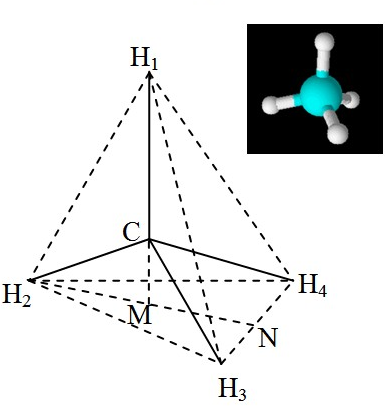
\includegraphics[width=3.35in,height=2.5in,viewport=14 14 250 190,clip]{Tetrahedron.eps}
\caption{\small Arrangement of the secant plane of constant energy in the method of tetrahedrons when $E_0\leqslant E\leqslant E_1$.}
\label{Tetrahedron}
\end{figure}

态密度的一般表达式为,
\begin{equation}
  N_A(E)=\frac1N\sum_{\vec k}A(\vec k)\delta(E-E(\vec k))=\frac{dD_A(E)}{dE}
  \label{eq:solid-198}
\end{equation}
这里
\begin{equation}
  D_A(E)=\frac1N\sum_{\vec k}A(\vec k)\theta(E-E(\vec k))
  \label{eq:solid-199}
\end{equation}
这里$\theta(x)$是Heavyside阶梯函数;$A(\vec k)$是关于矢量$\vec k$的任意函数。对应于式\eqref{eq:solid-197}的三种情况,
电子态密度的表达式分别为,
\begin{enumerate}
\item $E_0\leqslant E\leqslant E_1$
\begin{equation}
  \begin{split}
    N_A(E)=&\frac{|\vec k_{10}[\vec k_{20}\cdot\vec k_{30}]|}\Omega_0\frac{(E-E_0)^2/2}{(E_1-E_0)(E_2-E_0)(E_3-E_0)}\\
    &\cdot\left\{A_0+\left[\frac{A_1-A_0}{E_1-E_0}+\frac{A_2-A_0}{E_2-E_0}+\frac{A_3-A_0}{E_3-E_0}\right](E-E_0)/3\right\}
  \end{split}
  \label{eq:solid-200}
\end{equation}
\item $E_1\leqslant E\leqslant E_2$
\begin{equation}
  \begin{split}
    N_A(E)=&\frac{|\vec k_{10}[\vec k_{20}\cdot\vec k_{30}]|}\Omega_0\left\{\frac{(E-E_0)^2/2}{(E_1-E_0)(E_2-E_0)(E_3-E_0)}\right.\\
    &\cdot\left[A_0+\left(\frac{A_1-A_0}{E_1-E_0}+\frac{A_2-A_0}{E_2-E_0}+\frac{A_3-A_0}{E_3-E_0}\right)(E_3-E_0)/3\right]\\
    &-\frac{(E-E_1)^2/2}{(E_1-E_0)(E_2-E_1)(E_3-E_1)}\\
    &\cdot\left.\left[A_1+\left(\frac{A_1-A_0}{E_1-E_0}+\frac{A_2-A_1}{E_2-E_1}+\frac{A_3-A_1}{E_3-E_1}\right)\frac{(E-E_1)}3\right]\right\}
  \end{split}
  \label{eq:solid-201}
\end{equation}
\item $E_0\leqslant E\leqslant E_1$
\begin{equation}
  \begin{split}
    N_A(E)=&\frac{|\vec k_{10}[\vec k_{20}\cdot\vec k_{30}]|}\Omega_0\frac{(E_3-E)^2/2}{(E_3-E_0)(E_3-E_1)(E_3-E_2)}\\
    &\cdot\left\{A_3-\left[\frac{A_3-A_0}{E_3-E_0}+\frac{A_3-A_1}{E_3-E_1}+\frac{A_3-A_2}{E_3-E_2}\right](E_3-E)/3\right\}
  \end{split}
  \label{eq:solid-202}
\end{equation}
\end{enumerate}

二次插值方法选择一个大的立方体,%作为工作体积,
将该立方体分割为小的立方体,立方体的数目为$M^3$,这里$M$取决于计算要求的精度。用通过小立方体体心的三个剖面将每个小立方体分割出27个等价点,$\vec k$点的能量本征值$E(\vec k)$由27个点确定,$E(\vec k)$用小立方体内的一系列$\vec k$点展开到二阶,
\begin{equation}
  E(\vec k)=E_0+\vec m\vec k+\vec k\mathbf Q\vec k=\sum_{i=1}^{10}A_ia_i(\vec k)
  \label{eq:solid-203}
\end{equation}
这里$A_i$是展开系数;$a_i(\vec k)$是$\vec k_x$,$\vec k_y$,$\vec k_z$的线性组合到二阶。关于二次插值的详细介绍,可以参考文献\cite{AP67-15_1971}。

无论是线性插值还是二次插值,都有一些不足。对过渡金属,由于其复杂的能带结构,需要很多临界点(高对称性点)的解析结果,但是用线性插值方法则很难实现,而且态密度也主要由临界点决定,因此对临界点需要精确的解析。线性插值是对整个能带的解析积分,因此提高的是Fermi能级和Fermi面附近的态密度的计算精度。此外,线性插值方法方便处理非解析临界点(能带交叉点)的情况\cite{PLA28-570_1969,PRB7-891_1973,PRB5-1276_1972}。

能带交叉是积分误差的主要来源,在Brillouin区中接近交叉点的小区域内$|\nabla_{\vec k}E(\vec k)|\simeq0$,形成$N(E)$的能量奇点,导致不正确的插值计算,伴随能带交叉产生的另外一个问题是交叉点附近不同可观测物理量的矩阵元的行为。能带交叉导致矩阵元在交叉点变化剧烈,如果插值点位于这些交叉点上,可能引起更大的误差。理论上,计算精度可以通过增加线性插值的四面体数目或者二次插值中的参数$M$来提高,因此计算精度主要由布点数目决定。

四面体线性插值和二次插值是晶体计算中使用最多的积分方法。有时常将两种方法结合使用,用二次插值计算各参考点的线性插值部分,然后用线性四面体方法计算积分。与之类似的思想就是混合插值,用二次插值得到式\eqref{eq:solid-194}中的梯度
\begin{equation}
  \nabla E(\vec k)=\sum_{i=1}^{10}A_i\nabla C_i(\vec k)
  \label{eq:solid-204}
\end{equation}
这里$C_i(\vec k)$式$k_x$,$k_y$,$k_z$的简单解析函数。

\subsubsection{特殊点方法}
特殊点方法积分中用位于高对称性位置的$\vec k$点附近,以该特殊点作代表,用权重求和代替积分,所选择的权重要求与能带的能量无关,且对平滑函数产生最优化的收敛\cite{PRB13-5188_1976,PRB16-1748_1977}。

该方法最先应用于绝缘体,特殊点方法适用于这类能带变化平缓的体系。对于金属,由于Fermi面与部分能带交叉,导致Fermi面上某些占据能带在个别$\vec k$点能带不连续,如果直接应用特殊点积分收敛缓慢。这个问题可以通过人为展宽其Fermi面而得到克服。即用一个平滑函数替代一个阶梯函数,相当于考虑有限温度下的Fermi分布的情况。最优展宽$\Delta$既依赖于接近Fermi面能量$\varepsilon_F$附近的能带结构,也和所布特殊点的密度有关,一般通过估计Fermi能级$\varepsilon_F$的态密度$N(\varepsilon_F)$和不等价$\vec k$点数目$n_{\vec k}$来确定。注意到展宽应该使得本征值在给定的能量范围内保持平滑,即$\Delta\sim[n_{\vec k}N(\varepsilon_F)]^{-1}$。

特殊点方法的布点方案是用给定的倒格矢划分整个Brillouin区实现的。从$\Gamma$点出发,将每个方向都均分为$1/2$,由晶体的点群旋转,找出每一套由对称性相联系的等价$\vec k$点;通过空间群操作,将每一套等价$\vec k$中的代表性点移动到不可约Brillouin区,得到一组完全不等价的$\vec k$点,每个$\vec k$点的权重$w(\vec k)$等于等价$\vec k$点在总$\vec k$点中占的比重。

应用有限温度展宽的特殊点方法比起原始的四面体线性插值方法更有优势,因为只需要很少的高对称性点。而四面体方法包含的高对称性点的信息比起特殊点方法要少。对于体心立方(bcc)晶格,应用特殊点方法的时候,预先作一些特殊的处理,可以得到更快的收敛\cite{PRB8-5747_1973,Cohen-unpub}。

Bl\"ochl等改进了线性四面体插值积分方法\cite{PRB49-16223_1994}。提出了在已知空间群的情况下,用不可约$\vec k$点快速自动生成四面体的方案,避免了传统方法中分割四面体复杂过程。仿照特殊点方法,将积分变成不可约$\vec k$点的积分权重求和,
\begin{equation}
  \langle X\rangle=\frac1{\Omega_0}\sum_n\int_{\Omega_0}d^3kX_n(\vec k)f(\varepsilon_n(\vec k))=\sum_{jn}X_n(\vec k_j)w_{nj}
  \label{eq:solid-207}
\end{equation}
这里$X_n(\vec k_j)$是可观测量$\langle X\rangle$在不可约$\vec k$点的矩阵元:$X_n(\vec k)=\langle\Psi_n(\vec k)|X|\Psi_n(\vec k)\rangle$;
同时,Brillouin区中任意一点$\vec k$的函数值$X_n(\vec k)$可以通过四面体线性插值得到,
\begin{equation}
  X_n(\vec k)=\sum_jX_n(\vec k_j)w_j(\vec k)
  \label{eq:solid-208}
\end{equation}
$w_j(\vec k)$是四面体插值权重,当积分点在不可约点$\vec k_j$(或者其等价点)上时,插值权重为1,其余不可约点权重为零;在四面体内部,插值权重为线性函数。

积分权重的定义为:
$$w_{nj}(\vec k)=\frac1{\Omega_0}\int_{\Omega_0}d^3\vec kw_j(\vec k)f(\varepsilon_n(\vec k))$$
对于给定的能带,四面体方法的积分权重也只需计算一次。
Bl\"och提出了一个形式简单的积分校正公式,
\begin{equation}
  \delta\langle X\rangle=\sum_TD_T(\varepsilon_F)\frac1{40}\sum_{j=1}^4X_i\sum_{j=1}^4(\varepsilon_F-\varepsilon_i)
  \label{eq:solid-205}
\end{equation}
对应的积分权重校正为:
\begin{equation}
  dw_i=\frac{d\langle X\rangle}{d X_i}=\sum_T\frac1{40}D_T{\varepsilon_F}\sum_{j=1}^4(\varepsilon_F-\varepsilon_i)
  \label{eq:solid-206}
\end{equation}
可以很好的提高对金属的计算结果,而对绝缘体,用改进四面体积分方法用同等数量的布点,可以得到与特殊点方法相同的结果。

\subsection{晶体的总能量}
晶体总能量(不包括核的动能)可以分为两部分:一部分是原子核与芯电子组成的离子实能量,这部分能量基本上与晶体结构($\{\vec R\}$)无关,是一个常数,约为$-$$10^3$\,Ry/原子(在固体物理中讨论能量一般沿用Ry单位);另一部分是总能与离子实之差,即离子与价电子的相互作用、离子间的相互作用以及价电子间相互作用,约为$-$10\,Ry/原子。赝势(Pseudo Potential, PP)方法中常把总能量中不变的常数部分(即离子实的能量)设为零。晶体的结合能定义为这部分总能加上核的动能(通常是零点振动能)与孤立原子的能量差。在密度泛函理论中,赝势方法的晶体总能量$E_T$是晶格电子能量$E_{e\textrm{-}e}$与离子实排斥能$E_{N\textrm{-}N}$之和:
\begin{equation}
  E_T=E_{e\textrm{-}e}+E_{N\textrm{-}N}=T[\rho]+E_{ext}+E_{Coul}+E_{xc}+E_{N\textrm{-}N}
  \label{eq:solid-total}
\end{equation}
根据Kohn-Sham方程%\eqref{eq:dft-10}
,动能泛函用单电子能量表示为
\begin{equation}
  T[\rho]=\sum_i\langle\psi_i|E_i-V_{KS}|\psi\rangle
  \label{eq:solid-49}
\end{equation}
于是可以得到
\begin{equation}
  E_T=\sum_i\varepsilon_i-\frac12\iint d\vec rd\vec r'\dfrac{\rho(\vec r)\rho(\vec r')}{|\vec r-\vec r'|}+\int d\vec r\rho(\vec r)[\varepsilon_{xc}(\vec r)-V_{xc}(\vec r)]+E_{N\textrm{-}N}
  \label{eq:solid-50}
\end{equation}
在计算晶体总能量时,如果利用晶格的周期性,将实空间($\vec r$空间)总能量表示转换到动量空间($\vec k$空间)将使得计算十分便利。
\begin{equation}
  E_T=\sum_i\varepsilon_i-\frac{\Omega_0}2\sum_{\vec k\neq0}\rho^{\ast}(\vec k)V_{Coul}(\vec k)+\Omega_0\sum_{\vec k}\rho^{\ast}(\vec k)[\varepsilon_{xc}(\vec k)-V_{xc}(\vec k)]+E_{N\textrm{-}N}
  \label{eq:solid-51}
\end{equation}
这里$V_{Coul}(\vec k)$,$\varepsilon_{xc}(\vec k)$,$V_{xc}(\vec k)$和$\rho(\vec k)$分别是电子间Coulomb相互作用势、电子交换-相关能、交换-相关势和电子密度的Fourier分量,$\Omega_0$为原胞体积。其中电子间Coulomb势的Fourier分量$V_{Coul}(\vec k)$可以从Poisson方程
\begin{equation}
  \nabla^2V_{Coul}(\vec r)=-8\pi\rho(\vec r)
  \label{eq:poisson-r}
\end{equation}
用Fourier展开得到
\begin{equation}
  V_{Coul}(\vec k)=\dfrac{8\pi\rho(\vec k)}{k^2}
  \label{eq:poisson-k}
\end{equation}
对于交换-相关能和交换相关势,一般根据交换-相关能近似在实空间求得的$\varepsilon_{xc}(\vec r)$和$V_{xc}(\vec r)$后,用Fourier变换到动量空间,得到$\varepsilon_{xc}(\vec k)$和$V_{xc}(\vec k)$。

在实际计算中,需要必要的数学处理,因为离子间Coulomb相互作用能之和:
$$E_{N\textrm{-}N}=\dfrac12\sum_{\vec r,s}\sideset{}{'}\sum_{\vec R',s'}\dfrac{Z_sZ_{s'}}{|\vec R+\vec{\tau}_s-\vec R'-\vec{\tau}_{s'}|}$$
这里$Z_s$表示价电子数,$\vec R$表示晶格的格式,$\tau$表示原胞内的原子相对位矢。其求和包含无穷多项;此外$V_{Coul}(\vec k=0)$是发散的;而$V_{ext}$在不考虑其他外场,一般只考虑离子与电子的Coulomb相互作用,
\begin{equation}
  \begin{split}
    V_{ext}(\vec r)=&\sum_{\vec r,s}\dfrac{-2Z_s}{|\vec r-\vec R-\vec r_s|}=\sum_{\vec r,s}\dfrac{-2Z_s}{|\vec r-\vec R-\vec{\tau}_s|} \\
    =&\sum_{\vec r,s}v_{ext}'(\vec r-\vec R-\vec{\tau}_s)
  \end{split}
  \label{eq:solid-52}
\end{equation}
它的Fourier分量在$\vec k=0$也是发散的。由于这三项单独都是发散的,但因为整个系统处于电中性,这些发散项相互抵消,是一个常数。因此在解Kohn-Sham方程的时候,可先将$V_{Coul}(\vec k=0)$和$V_{ext}(\vec k=0)$同时置为零,这相当于将势能作一平移,或者说重新定义真空能级,而在总能量计算中补偿这一平移。记这些发散项的和为:
\begin{equation}
  \begin{split}
    \lim\limits_{\vec k\rightarrow0}&\Omega_0\left[\dfrac12V_{Coul}(\vec k)+\sum_sv_{ext}^s(\vec k)\right]\rho(\vec k)+\dfrac12\sum_{\vec R,s}\sideset{}{'}\sum_{\vec R',s'}\dfrac{2Z_sZ_{s'}}{|\vec R+\vec{\tau}_s-\vec R'-\vec{\tau}_{s'}|} \\
    &=\sum_s\alpha_s\sum_sZ_s+E_{Ewald}
  \end{split}
  \label{eq:solid-53}
\end{equation}

对于形如$Z_s/r$的外场,它的Fourier分量在$\vec k=0$附近展开:$v_{ext}^s(\vec k)=-\dfrac{8\pi Z_s}{\Omega_0k^2}+\alpha_s+o(\vec k)$,同样的展开$\rho(\vec k)$,有$\lim\limits_{\vec k\rightarrow0}\rho(\vec k)=\dfrac{\sum\limits_sZ_s}{\Omega_0}+\beta k^2+o(\vec k)$,代入式\eqref{eq:solid-53},去掉$\vec k$的高次项,有
\begin{equation}
  \begin{split}
    \lim\limits_{\vec k\rightarrow0}&\biggl[\dfrac{\Omega_0}2\dfrac{8\pi\rho^2(\vec k)}{k^2}+\Omega_0\left(\dfrac{-8\pi\sum\limits_sZ_s}{\Omega_0k^2}+\sum_s\alpha_s\right)\rho(\vec k)+\frac12\dfrac{8\pi(\sum\limits_sZ_s)^2}{\Omega_0k^2}\biggr]\\
    &+\frac12\sum_{\vec R,s}\sideset{}{'}\sum_{\vec R',s'}\dfrac{2Z_sZ_{s'}}{|\vec R+\vec{\tau}_s-\vec R'-\vec{\tau}_{s'}|}-\lim\limits_{\vec k\rightarrow0}\frac12\dfrac{8\pi(\sum\limits_sZ_s)^2}{\Omega_0k^2}\\
    =&\sum_s\alpha_s\sum_sZ_s+E_{Ewald}
  \end{split}
  \label{eq:solid-54}
\end{equation}
其中离子间排斥能可用Ewald方法得到\cite{Born-Huang}:
\begin{equation}
  \begin{split}
    E_{Ewald}=&\frac12\sum_{\vec R,s}\sideset{}{'}\sum_{\vec R',s'}\dfrac{2Z_sZ_{s'}}{|\vec R+\vec{\tau}_s-\vec R'-\vec{\tau}_{s'}|}-\lim\limits_{\vec k\rightarrow0}\frac12\dfrac{8\pi(\sum\limits_sZ_s)^2}{\Omega_0k^2} \\
    =&\frac12\sum_{\vec R,s}\sideset{}{'}\sum_{\vec R',s'}\dfrac{2Z_sZ_{s'}}{|\vec R+\vec{\tau}_s-\vec R'-\vec{\tau}_{s'}|}-\frac1{\Omega_0}\sum_{s,s'}\int d\vec r\frac{Z_sZ_{s'}}r \\
    =&\sum_{s,s'}Z_sZ_{s'}\left\{\frac{4\pi}{\Omega_0}\sum_{\vec k\neq0}\cos[\vec k\cdot(\vec{\tau}_s-\vec{\tau}_{s'})]\dfrac{e^{-k^2/4\eta^2}}{k^2}\right.\\
    &-\left.\frac{\pi}{\eta^2\Omega_0}+\frac12\sum_{\vec r}\left.\dfrac{erf(\eta x)}x\right|_{\vec R+\vec{\tau}_s-\vec{\tau}_{s'}\neq0}-\dfrac{2\eta}{\sqrt{\pi}}\delta_{s,s'}\right\}
  \end{split}
  \label{eq:solid-55}
\end{equation}
这里$erf(x)$是误差函数,参数$\eta$原则上是任意的,如果$\vec r$取得足够多,上述求和是与$\eta$无关的。一般选取$\eta$使得在正格子和倒格子空间收敛得足够快。而$\alpha_s$可根据实际的$v_{ext}^s(\vec r)$得到:
\begin{equation}
  \alpha_s=\lim\limits_{\vec k\rightarrow0}\left[v_{ext}^s(\vec k)+\dfrac{8\pi Z_s}{\Omega_0k^2}\right]=\dfrac1{\Omega_0}\int d\vec r\left[v_{ext}^s(\vec r)+\dfrac{2Z_s}r\right]
  \label{eq:solid-56}
\end{equation}
由此得到总能量
\begin{equation}
  \begin{split}
   E_T=&\sum_i\varepsilon_i-\dfrac{\Omega_0}2\sum_{\vec k\neq0}\rho^{\ast}(\vec k)V_{Coul}(\vec k)+\Omega_0\sum_{\vec k}\rho^{\ast}(\vec k)[\varepsilon_{xc}(\vec k)-V_{xc}(\vec k)]\\
   &+\sum_s\alpha_s\sum_sZ_s+E_{Ewald}
  \label{eq:solid-57}
  \end{split}
\end{equation}

全势方法同样改进了求解Madelung势能的计算方法\cite{JMP22-2433_1981}。MT近似下,WS原胞内中MT球的球心位于$\vec\gamma_{\nu}$,$R_{\nu}$为半径。如果球面上的势能平均为$S_0(R)$,除去球心核电荷以外所有电荷在MT球面上产生的势能平均为:
\begin{equation}
  S(R_{\nu})\equiv S_0(R_{\nu})+Z_{\nu}/R_{\nu}
  \label{eq:solid-79}
\end{equation}
则根据$S(R_{\nu})$和球形Dirichlet边值问题\cite{JMP22-2433_1981},球心$\vec\gamma_{\nu}$处的Madelung势(因为要求的Madelung势位于球心,只有$l=0$部分对此有贡献,故只需考虑$S(R_{\nu})$的球形平均部分)为\cite{PRB26-4571_1982}:
\begin{equation}
  \begin{split}
   V_M(\vec\gamma_{\nu})&=\frac1{R_{\nu}}[R_{\nu}S_0(R_{\nu})+Z_{\nu}-Q_{\nu}]+\sqrt{4\pi}\int_0^{R_{\nu}}drr\rho_{00}(r_{\nu})\\
   &=\frac1{R_{\nu}}[R_{\nu}S_0(R_{\nu})+Z_{\nu}-Q_{\nu}]+\bigg\langle\frac1r\rho(\vec r)\bigg\rangle_{\nu}
  \end{split}
   \label{eq:Madelung}
\end{equation}
其中$Q_{\nu}$表示MT球内的电子电荷之和。$\rho(\vec r)$是MT球内的电荷密度,可以用球谐函数表示为
\begin{equation}
  \rho(\vec r_{\nu})=\sum_{lm}\rho_{lm}(r_{\nu})Y_{lm}(\hat r_{\nu})
  \label{eq:solid-80}
\end{equation}
类似地,WS原胞内的总能量可以表示为:
\begin{equation}
  \begin{split}
   E_T=&\sum_i\varepsilon_i-\frac12\int_{\Omega_0}\rho(\vec r)[V_c(\vec r)+2\mu_{xc}(\vec r)]d\vec r-\frac12\sum_{\nu}Z_{\nu}V_M(\vec\gamma_{\nu})+E_{xc}[\rho] \\
   =&\sum_i\varepsilon_i-\frac12\left(\int_{\Omega_0}\rho(\vec r)V_c(\vec r)d\vec r+\sum_{\nu}Z_{\nu}\bigg\langle\frac1r\rho(\vec r)\bigg\rangle_{\nu}\right)-\int_{\Omega_0}\rho(\vec r)\mu_{xc}(\vec r)d\vec r\\
   &-\frac12\sum_{\nu}\frac{Z_{\nu}}{R_{\nu}}[R_{\nu}S_0(R_{\nu})+Z_{\nu}-Q_{\nu}]+E_{xc}[\rho]
  \end{split}
  \label{eq:solid-81}
\end{equation}
这里$V_c(\vec r)=\int\dfrac{\rho(\vec r')}{|\vec e-\vec r'|}d\vec r'-\sum\limits_{\alpha}\dfrac{Z_{\alpha}}{|\vec r-\vec r_{\alpha}|}$。总能量写成这样的形式,原子核位置的Coulomb势奇点可以排除。将势能和电荷密度在各原子核附近作球谐展开,在原子核附近,有
\begin{displaymath}
  \begin{split}
    &\int_{\Omega_0}\rho(\vec r)V_c(\vec r)d\vec r+Z{\nu}\sqrt{4\pi}\int_0^{R_{\nu}}drr^2\frac{\rho_{00}(r)}r\\
    =&\sqrt{4\pi}\int_{\Omega_0}drr^2\rho_{00}(\vec r)\left(V_{00}(r)Y_{00}(\hat r)+\frac{Z_{\nu}}r\right)+\sum_{lm>0}\int drr^2\rho_{lm}(r)V_{lm}(r)
  \end{split}
\end{displaymath}
Coulomb势的奇点只出现在$V_{00}(r)$中,将$V_{00}(r)$写成核的点电荷势与源于电子的平滑势两部分之和,有
$$V_{00}(r)=-\sqrt{4\pi}\frac{Z_{\nu}}r+\hat V_{00}(r)$$
有必要指出的是,通过这样的方式,可以将总能量中的奇点排除,但是单独每一项在原子核位置能量仍然是发散的。

如果采用标准的LDA近似,式\eqref{eq:solid-81}交换-相关能可以写成:
\begin{equation}
  E_{xc}[\rho]\approx\int_{\Omega_0}\rho(\vec r)\varepsilon_{xc}(\vec r)d\vec r
  \label{eq:solid-82}
\end{equation}

一般地,总能量计算在动量空间中完成。在MT近似下,间隙区的电荷密度用平面展开,有
$$\rho(\vec r)=\sum_{\vec G}e^{i\vec G\cdot\vec r},\quad \vec r\in\mathrm{Interstitial}$$
在MT球内,电荷密度用球谐函数展开,在动量空间中的展开形式为:
$$\bar\rho_{lm}(r_{\nu})=4\pi i^l\sum_{\vec G}\rho(\vec G)e^{i\vec G\cdot\vec{\gamma}_{\nu}}j_l(Gr_{\nu})Y_{lm}^{\ast}(\vec G)$$
于是,WS原胞内的晶体总能量可以写成:
\begin{equation}
  \begin{split}
  E=&\sum_i\varepsilon_i-\sum_{\vec G}\Omega_0\rho(\vec G)-\frac12\sum_{\nu}\dfrac{Z_{\nu}}{R_{\nu}}[Z_{\nu}-Q_{\nu}+R_{\nu}S_0(R_{\nu})]\\
  &-\sum_{\nu}\sum_{lm}\int_0^{R_{\nu}}drr^2\left[\rho_{lm}(r_{\nu})\left(\tilde V_{lm}^{\ast}(r_{\nu})\dfrac{\sqrt{4\pi}}{2r_{\nu}}Z_{\nu}\delta_{l0}\right)-\bar\rho_{lm}(\vec r_{\nu})\bar V_{lm}^{\ast}(\vec r_{\nu})\right]
  \end{split}
  \label{eq:solid-83}
\end{equation}
这里$\tilde V(\vec r)$和$\bar V_{lm}(\vec r)$根据下式计算:
$$\tilde V(\vec r)=\frac12V_c(\vec r)-\varepsilon_{xc}(\vec r)+\mu_{xc}(\vec r)$$

\subsection{LDA+U和GW近似}

\subsubsection{LDA+U方法}
LDA近似和精确密度泛函方法的差别在于,后者电子数$N$改变整数值\cite{PRL49-1691_1982}的时候,势能的改变是不连续的;而LDA近似中势能是电子数$N$的连续函数。因为不具备势能随电子数变化不连续的特征,LDA方法在描述含有{\it d}\,或{\it f}\,电子的过渡金属和稀土元素化合物体系时常常失效。Gunnarsson和Schonhammer\cite{PRL56-1968_1986}证明,单电子势的不连续对能带的带隙有很大的贡献。LDA近似的另一个不足在于,LDA计算得到的轨道能量(定义为能量$E$对轨道占据数$n_i$的导数,即$\varepsilon_i=\partial E/\partial n_i$),不符合Koopmans定理,与实验或者严格计算得到的轨道能量差别很大,但是LDA方法得到的总能量一般与实验结果符合的较好。一个典型的例子就是对H原子的计算结果,LDA计算的轨道能为$-$0.54\,Ry(实际结果为$-$1.0\,Ry),总能量($-$0.976\,Ry)则非常接近$-$1.0\,Ry\cite{PRB37-9919_1988}。文献\cite{PRB44-943_1991}提出通过对LDA势加入轨道校正克服LDA方法的不足(称为LDA+U方法)。LDA+U方法与Andersen掺杂模型\cite{PR124-41_1961}思想相同,对局域的{\it d}\,或{\it f}\,电子,采用模型Hamiltonian方法考虑$d$-$d$或$f$-$f$间相互作用(定域Coulomb相互作用U),离域的{\it s}\,和{\it p}\,电子的运动用LDA近似描述。

Herring讨论了$U$值的物理意义\cite{Herring},含有$n$个3{\it d}\,电子的原子中,U值定义为两个原子间转移一个{\it d}\,电子的能量,即$$2(d^n)\rightarrow d^{n+1}+d^{n-1}$$

对{\it d}\,电子数目可以变化的离子体系$d$-$d$电子间的相互作用LDA表示为$E=UN(N-1)/2$\cite{PRB48-16929_1993},将总能量中扣除LDA的$d$-$d$电子相互作用,再加上局域的电子间相互作用,可有
\begin{equation}
  E=E_{LDA}-UN(N-1)/2+\frac12U\sum_{i\neq j}n_in_j
  \label{eq:solid-251}
\end{equation}
由式\eqref{eq:solid-251}对轨道占据数$n_i$求导得轨道能
\begin{equation}
  \varepsilon_i=\frac{\partial E}{\partial n_i}=E_{LDA}+U(\frac12-n_i)
  \label{eq:solid-252}
\end{equation}
该式将占据态轨道($n_i$=1)和非占据态轨道($n_i$=0)的LDA轨道能分别移动-U/2和+U/2,由此得到的轨道相关势[$V_i(\vec r)=\delta E/\delta n_i(\vec r)$]为
\begin{equation}
  V_i(\vec r)=V_{LDA}(\vec r)+U(\frac12-n_i)
  \label{eq:solid-253}
\end{equation}
式\eqref{eq:solid-253}保持了精确密度泛函理论的单电子势能的不连续行为。

式\eqref{eq:solid-251}没有考虑相同自旋电子的交换作用。设自旋$\sigma$的{\it d}-{\it d}\,电子间交换参数为{\it J}\,,则{\it N}\,电子的LDA近似下{\it d}-{\it d}\,相互作用为$UN(N-1)/2-JN(N-2)/4$。

如果考虑Coulomb势和交换势的非球形部分的贡献(与{\it d}\,轨道的$m$和$m'$相关部分),引入矩阵元$U_{mm'}$和$J_{mm'}$,有
\begin{equation}
  U_{mm'}=\sum_ka_kF^k
  \label{eq:solid-210}
\end{equation}
\begin{equation}
  J_{mm'}=\sum_kb_kJ^k
  \label{eq:solid-211}
\end{equation}
\begin{equation}
  a_k=\frac{4\pi}{2k+1}\sum_{q=-k}^k\langle lm|Y_{kq}|lm\rangle\langle lm|Y_{kq}^{\ast}|lm'\rangle
  \label{eq:solid-212}
\end{equation}
\begin{equation}
  b_k=\frac{4\pi}{2k+1}\sum_{q=-k}^k|\langle lm|Y_{kq}|lm'\rangle|^2
  \label{eq:solid-213}
\end{equation}
这里$F^k$是Slater积分,$\langle lm|Y_{kq}|lm'\rangle$是三个球谐函数$Y_{lm}$的乘积的积分。

由此得到的总能量为
\begin{equation}
  \begin{split}
  E=&E_{LDA}-[UN(N-1)/2-JN(N-2)/4]\\
  &+\frac12\sum_{m,m',\sigma}U_{mm'}n_{m\sigma}n_{m'\sigma}\\
  &+\frac12\sum_{m\neq m',m',\sigma}(U_{mm'}-J_{mm'})n_{m\sigma}n_{m'\sigma}
  \end{split}
  \label{eq:solid-214}
\end{equation}
式\eqref{eq:solid-214}应占据数$n_{m\sigma}$求导,得到轨道相关的单电子势能
\begin{equation}
  \begin{split}
    V_{m\sigma}(\vec r)=&V_{LDA}(\vec r)+\sum_{m'}(U_{mm'}-U_{eff})n_{m-\sigma}\\
    &\sum_{m\neq m'}(U_{mm'}-J{mm'}-U{eff})n_{m\sigma}+U_{eff}\left(\frac12-n_{m\sigma}\right)-\frac12J
  \end{split}
  \label{eq:solid-215}
\end{equation}
这里$U_{eff}=U-J/2$。

为了计算矩阵元$U_{mm'}$和$J_{mm'}$,必须知道Slater积分$F^k$(对{\it d}\,电子是$F^0$,$F^2$和$F^4$)。文献\cite{PRB43-7570_1991}用超晶胞近似(supercell approximation)给出Coulomb参数$U$,和$F^0$相等,将矩阵元$U_{mm'}$和$(U_{mm'}-J_{mm'})$对所有$mm'$求平均,可以得到$U$和$(U-J)$,根据Clebsch-Gordan系数性质,有平均值为
\begin{equation}
  U=\frac1{(2l+1)^2}\sum_{mm'}U_{mm'}=F^0
  \label{eq:solid-216}
\end{equation}
\begin{equation}
  U-J=\frac1{2l(2l+1)}\sum_{mm'}(U_{mm'}-J_{mm'})=F^0-(F^2+F^4)
  \label{eq:solid-217}
\end{equation}
\begin{equation}
  J=(F^2=F^4)/4
  \label{eq:solid-218}
\end{equation}
为了由$U$和$J$得到所有的Slater积分,只需要知道$F^4/F^2$\cite{PRB42-5459_1990}。

LDA+U方法最重要的特征是具备了单电子势的不连续性。计算表明LDA+U方法对含有定域强Coulomb相互作用的体系是可靠的\cite{PRB48-16929_1993,JPCS56-1521_1995,EPL36-551_1996}。无论对含有近芯层的局域4{\it f}\,电子的稀土金属离子还是对过渡金属的氧化物(金属的3{\it d}\,电子与氧原子2{\it p}\,轨道有很强的相互作用)体系都有效。尽管LDA+U方法是平均场近似,并不足以描述金属-绝缘体的Mott转变和具有强关联的金属。但对诸如FeSi和LaCaO$_3$,LDA+U仍能够给出有关于金属-绝缘体转变的有用信息\cite{JPCM9-767_1997}。甚至对含有5{\it f}\,电子的化合物的研究也取得一定的成功\cite{PRB54-R3706_1996}。

\subsubsection{GW近似}
Landau的Fermi液体理论是研究群体激发和多体Fermi子体系物理性质的重要方法\cite{Landau}。Fermi液体的特征是准粒子分布$\varepsilon=\varepsilon(\vec k)$由体系总能量$E$对分布函数的变分,即
\begin{equation}
  \frac{\delta E}{\delta n(\vec k)}=\varepsilon(\vec k)
  \label{eq:solid-219}
\end{equation}
关联函数$f(\vec k,\vec k')$由准粒子能量对整个$\vec k$空间粒子分布变分得到
\begin{equation}
  \frac{\delta\varepsilon(\vec k)}{\delta n(\vec k')}=\frac{\delta^2E}{\delta n(\vec k)\delta n(\vec k')}=f(\vec k,\vec k')
  \label{eq:solid-220}
\end{equation}
考虑准粒子间相互作用,体系激发能记作
\begin{equation}
  W=\sum_{\vec k}\varepsilon(\vec k)\delta n(\vec k)+\frac12\sum_{\vec k}\sum_{\vec k'}f(\vec k,\vec k')\delta n(\vec k)\delta(\veck')
  \label{eq:solid-221}
\end{equation}

Green函数是研究Fermi液体的重要数学工具。对宏观体系,Green函数定义为\cite{Lifshitz}
\begin{equation}
  \tilde G(x,x')=-i\langle T\hat\Psi(x)\hat\Psi^{\ast}(x')\rangle
  \label{eq:solid-222}
\end{equation}
这里$x$表示时间$t$和位置$\vec r$,$\langle\cdots\rangle$表示对体系基态求平均,$T$表示按时间先后乘积算符。$\hat\Psi$是Heisenberg算符,对式\eqref{eq:solid-222}进行Fourier变换,得到以$\vec r$,$E$为表象的Green函数$\tilde G(\vec r,\vec r';E)$是Dyson方程\cite{Lifshitz}
\begin{equation}
  (\nabla^2+E)\tilde G(\vec r,\vec r';E)-\int d\vec r''\Sigma(\vec r,\vec r'';E)\tilde G(\vec r'',\vec r';E)=\delta(\vec r-\vec r')
  \label{eq:solid-223}
\end{equation}
的解。这里$\Sigma(\vec r,\vec r';E)$是描述交换和相关效应的质量或自能算符,这是个与能量有关的非定域的非-Hermitian算符,考虑到粒子与体系中其他粒子的相互作用。晶体中的质量具有平移对称性,
\begin{equation}
  \Sigma(\vec r+\vec a,\vec r+\vec a;E)=\Sigma(\vec r,\vec r';E),
  \label{eq:solid:224}
\end{equation}
这里$\vec a$是晶体平移格矢。

临近Green函数的极点,式\eqref{eq:solid-223}右面的$\delta$函数为0,所得积分-微分方程的本征值确定体系激发能谱\cite{Lifshitz,PR145-561_1966}
\begin{equation}
  -\delta^2\Phi_{\vec k}(\vec r,E)+\int d\vec r'\Sigma(\vec r,\vec r';E)\Phi_{\vec k}(\vec r',E)=\varepsilon_{\vec k}\Phi_{\vec k}(\vec r,E) 
  \label{eq:solid-225}
\end{equation}
这里函数$\Phi_{\vec k}(\vec r,E)$类似于周期场中的单电子Bloch波函数。对金属中的Fermi电子液体中用式\eqref{eq:solid-225}替代一般Schr\"odinger方程。与一般的Schr\"odinger方程不同,式\eqref{eq:solid-225}的能量本征值是复数,因为质量算符$\Sigma(\vec r,\vec r';E)$是复数。

由式(\ref{eq:solid-223},\ref{eq:solid-225})得到Green函数
\begin{equation}
  \tilde G(\vec r,\vec r';E)=\sum_{\vec k}\frac{\Phi_{\vec k}(\vec r,E)\Phi_{\vec k}^{\ast}(\vec r',E)}{E-\varepsilon_{\vec k}(E)+i0\mathrm{sign}E}
  \label{eq:solid-226}
\end{equation}
$\varepsilon_{\vec k}(E)$是体系中加入一个粒子引起的能量改变。如果将单个准粒子改变引起得能量变化$\varepsilon_{\vec k}(E)$定义为式\eqref{eq:solid-219}中的准粒子能量,对临近Fermi面的态,函数$\tilde G(\vec r,\vec r';E)$在$E=\varepsilon_{\vec k}(E)$有极值。因此Green函数极值确定了多Fermi子体系的元激发能谱。一般说,因为和其他粒子相互作用,准粒子能量为复数。复数能量使得体系激发态的寿命有限$(\tau\sim1/|\mathrm{Im}\varepsilon|)$\cite{Landau-Lifshitz}。能量宽度由$\mathrm{Im}\varepsilon$确定。

%临近Fermi能级,$\mathrm{Im}\varepsilon_{\vec k}(E)\rightarrow0$,相应的$\mathrm{Im}\Sigma\rightarrow0$,于是解方程\eqref{eq:solid-225}得到$\mathrm{Re}\varepsilon_{\vec k}(E)$和实数形式的$\Sigma(\vec r,\vec r';E)$和$\epsilon_{\vec k}(E)$。

根据Hohenberg-Kohn定理,本征值$\Sigma(\vec r,\vec r';E)$由体系基态确定,它也是电子密度的函数。Sham和Kohn建议可用局域电子密度近似表示$\Sigma(\vec r,\vec r';E)$\cite{PR145-561_1966}:
\begin{equation}
  \Sigma(\vec r,\vec r';E)=V_C(\vec r)\delta(\vec r-\vec r')+\Sigma_0(\vec r-\vec r';E-V_C(\vec r_0);\rho(\vec r_0))
  \label{eq:solid-227}
\end{equation}
这里$\Sigma_0$是密度为$\rho$的无相互作用电子气的本征能量,$V_C(\vec r_0)$是位于$\vec r_0=(\vec r+\vec r')/2$的静电Coulomb势。此外式\eqref{eq:solid-227}已将能量$\Sigma$中的局域部分以Hartree势的形式分离出来,因此可以利用$\Sigma_0$的短程效应。

对本征函数$\Phi_{\vec k}$作近似
$$\Phi_{\vec k}(\vec r,E)=A(\vec k)\exp[i\vec p(\vec r)\vec r]$$
并认为$A$和电子动量与$\vec r$无关,将式\eqref{eq:solid-225}称为类似Kohn-Sham方程的表达式\cite{JPC4-2064_1971},
\begin{equation}
  [-\nabla^2+V_C(\vec r)+\Sigma_{xc}(\rho(\vec r),E)]\Phi_{\vec k}(\vec r,E)=\varepsilon_{\vec k}(\vec r,E)
  \label{eq:solid-228}
\end{equation}
若$E=\mu$,$\Sigma_{xc}(\rho(\vec r),\mu)\equiv\mu_{xc}(\rho(\vec r))$我们因此得到符合局域密度近似的DFT方程,两者的交换-相关势$\mu_{xc}$是相同的。因此对于低激发能,可以使用近似$\Sigma_{xc}(\rho(\vec r),E)\simeq\mu_{xc}$,此结果对应于忽略准粒子间的相互作用,即Landau函数$f(\vec k,\vec k')=0$。

因此基于DFT的能带计算,如果充分考虑交换-相关效应,可以计算多电子体系的元激发能量。注意,采用单电子近似,要求能带比较宽,即中心位于不同格点的波函数有较大的重叠,电子间相互作用不是很强。

Hedin和Lundqvist详细回顾了用Green函数技术解决电子相关的问题\cite{Hedin-Lundqvist}。在单粒子近似下的Green函数,准粒子与谱函数的峰联系在一起。如果峰足够尖锐,表明存在一个明确的准粒子能量,对一般的非均匀体系,准粒子能量和波函数可以通过解Dyson方程\eqref{eq:solid-225}求得。对于准粒子问题,核心问题是对自能算符$\Sigma(\vec r,\vec r';E)$的足够好的近似。常用的方法是GW近似\cite{PR139-A796_1965},自能用屏蔽相互作用$W$计算到最低阶。
\begin{equation}
  \Sigma(\vec r,\vec r';E)=\frac i{2\pi}\int_{-\infty}^{\infty}dE'\tilde G(\vec r,\vec r';E+E')W(\vec r,\vec r';E')
  \label{eq:solid-229}
\end{equation}
Green函数$\tilde G$由准粒子的波函数和能量表示,屏蔽Coulomb作用$W$
\begin{equation}
  W(\vec r,\vec r';E)=\frac1{\Omega}\int d^3r''\varepsilon^{-1}(\vec r,\vec r'';E)V(\vec r''-\vec r')
  \label{eq:solid-230}
\end{equation}
这里$V$是未屏蔽的Coulomb势,$\varepsilon^{-1}$是介电函数矩阵的逆阵,
\begin{equation}
  \varepsilon^{-1}(\vec r,\vec r';E)=\delta(\vec r-\vec r')+\int d^3r''V(\vec r'-\vec r'')P(\vec r'',\vec r';E)
  \label{eq:solid-231}
\end{equation}
这里$P$是完全响应函数,于是
\begin{equation}
  W(\vec r,\vec r';E)=V(\vec r-\vec r')+W_c(\vec r,\vec r';E)
  \label{eq:solid-232}
\end{equation}
这里
\begin{equation}
  W_c(\vec r,\vec r;E)=\int d^3r_1d^3r_2V(\vec r'-\vec r_1)P(\vec r_1,\vec r_2;E)V(\vec r_2-\vec r')
  \label{eq:solid-233}
\end{equation}
Green函数可以写成谱表示
\begin{equation}
  G(\vec r,\vec r';E)=\int_{-\infty}^{\mu}dE'\frac{A(\vec r,\vec r';E')}{E-E'-i\delta}+\int_{\mu}^{\infty}dE'\frac{A(\vec r,\vec r';E')}{E-E'+i\delta}
  \label{eq:solid-234}
\end{equation}
这里$A(\vec r,\vec r';E)=-\frac1{\pi}\mathrm{Im}G(\vec r,\vec r';E)\mathrm{sgn}(E-\mu)$

实际计算中,取零阶Green函数,有
\begin{equation}
  A(\vec r,\vec r';E)=\sum_{kn}\psi_{kn}(\vec r)\psi_{kn}^{\ast}(\vec r')\delta(E-E_{kn})
  \label{eq:solid-235}
\end{equation}
于是自能可以写成
\begin{equation}
  \Sigma(\vec r,\vec r';E)=\Sigma_x(\vec r,\vec r')+\Sigma_c(\vec r,\vec r';E)
  \label{eq:solid-236}
\end{equation}
这里$\Sigma_x$是净的交换势,
\begin{equation}
  \Sigma_x(\vec r,\vec r')=-\sum_{kn}^{occ}\psi_{kn}(\vec r)\psi_{kn}^{\ast}(\vec r')V(\vec r-\vec r')
  \label{eq:solid-254}
\end{equation}
$E_c$自能的相关部分,
\begin{equation}
  \begin{split}
    \Sigma_c(\vec r,\vec r';E)=&\sum_{kn}^{occ}\psi_{kn}(\vec r)\psi_{kn}^{\ast}(\vec r')W_c^-(\vec r,\vec r';E-E_{kn})\\
    &+\sum_{kn}^{occ}\psi_{kn}(\vec r)\psi_{\vec r}^{\ast}(\vec r')W_c^+(\vec r,\vec r';E-E_{kn})
  \end{split}
  \label{eq:solid-237}
\end{equation}
其中$W_c^{\pm}(\vec r,\vec r';E)=\dfrac i{2\pi}\displaystyle\int_{-\infty}^{+\infty}dE'\frac{W_c(\vec r,\vec r';E')}{E+E'\pm i\delta}$。于是$\Sigma(\vec r,\vec r';E)$可以记作\cite{JPCM9-767_1997},
\begin{displaymath}
  \Sigma(\vec r,\vec r';E)=-\sum_{kn}\psi_{kn}(\vec r)\psi_{kn}^{\ast}(\vec r')W_0(\vec r,\vec r';E-E_{kn})
\end{displaymath}
其中
\begin{displaymath}
  \begin{split}
    W_0(\vec r,\vec r';E-E_{kn})\equiv&[V(\vec r-\vec r')-W_c^-(\vec r,\vec r';E-E_{kn})]\theta(\mu-E_{kn})\\
    &-W_c^+(\vec r,\vec r';E-E_{kn})\theta(E_{kn}-\mu)
  \end{split}
\end{displaymath}
这样的GWA近似的自能与Hartree-Fock方法具有相同的形式,但是自能是能量的函数且因为包含相关作用,因此也依赖于未占据态。GWA可以看作是包含动态屏蔽Coulomb势$W_0$的推广Hartree-Fock方法,注意这里的$W_0$与动态屏蔽势$W$不同。

在各种能带计算方法中引入GW近似,包括赝势方法\cite{PRB34-5390_1986},LMTO-TB方法\cite{PRL74-3221_1995}。GWA校正主要应用于简单金属和过渡金属体系,但由于计算过程比较复杂所以目前还没有广泛应用到复杂体系的计算中。GWA校正的另一个问题是计算屏蔽相互作用所需的响应函数,要借助LDA得到的波函数和能带来计算得到\cite{JPCM9-767_1997}。但是这样的方法只适用于电子相关较小的体系(比如绝缘体或者半导体);对电子强相关体系,则需要采用比LDA近似更好的Hamiltonian,一般可以通过自洽迭代来计算自能\cite{PRL74-3221_1995}。

\subsubsection{LDA+U和GWA校正的关系}
尽管GWA是由多体微扰理论导出的最简单的自能近似,但是计算量已经很大。GWA和LDA+U可以分别看作包含依赖于频率和轨道屏蔽Coulomb作用的Hartree-Fock方法。至少对含有局域的{\it d}\,或{\it f}\,轨道的过渡金属和稀土金属离子,LDA+U可以看作是对GWA的近似\cite{JPCM9-767_1997}。

LDA+U是针对包含在离域态中的定域态轨道的自能校正,定域态的强Coulomb相关用参数$U$校正,而离域态可以用LDA很好的描述。为了确定LDA+U和GWA之间的关系,对态$\psi_d$,考虑GWA中自能的相关部分
\begin{equation}
  \begin{split}
    \langle\psi_d|\Sigma_c(E_d)|\psi_d\rangle=&\langle\psi_d\psi_d|W_c^-|\psi_d\psi_d\rangle\\
    &+\sum_{kn\neq d}^{occ}\langle\psi_d\psi_{kn}|W_c^-(E_d-E_{kn})|\psi_{kn}\psi_d\rangle\\
    &+\sum_{kn}^{unocc}\langle\psi_d\psi_{kn}|W_c^+(E_d-E_{kn})|\psi_{kn}\psi_d\rangle
  \end{split}
  \label{eq:solid-238}
\end{equation}
严格地说,自能应该是$\tilde E_d=E_d+$自能校正。如果$\psi_d$是局域的而且能量与其他态很好的分离,则式\eqref{eq:solid-238}第一项比剩下的其余项大得多,最后一项含未占据的$\psi_d$态,但因为这些项与占据态正交,因此这一项比第一项小得多。可作近似\cite{JPCM9-767_1997}
\begin{equation}
  \langle\psi_d|\Sigma_c(E_d)|\psi_d\rangle\approx\langle\psi_d\psi_d|W_c^-(0)|\psi_d\psi_d\rangle=-\frac12\langle\psi_d\psi_d|W_c(0)|\psi_d\psi_d\rangle
  \label{eq:solid-239}
\end{equation}
将屏蔽势关联部分写成谱函数表象,
\begin{equation}
  W_c(E)=\int_{-\infty}^0dE'\frac{B(E')}{E-E'-i\delta}+\int_0^{\infty}dE'\frac{B(E')}{E-E'+i\delta}
  \label{eq:solid-240}
\end{equation}
这里$B(E)=-\dfrac1{\pi}W_c(E)\mathrm{sgn}(E)$。
$W_c$是$E$的偶函数,因此$B(E)$是奇函数,因此$W_c^-(0)=-1/2W_c(0)$,类似的对未占据的{\it d}\,态,有$+1/2\langle\psi_d\psi_d|W_c(0)|\psi_d\psi_d\rangle$,因此能量差为
\begin{equation}
  \begin{split}
    \Delta&=E_2^{HF}-E_1^{HF}+\langle\psi_d\psi_d|W_c(0)|\psi_d\psi_d\rangle\\
    &=\langle\psi_d\psi_d|V|\psi_d\psi_d\rangle+\langle\psi_d\psi_d|W_c(0)|\psi_d\psi_d\rangle\\
    &=\langle\psi_d\psi_d|W(0)|\psi_d\psi_d\rangle
  \end{split}
  \label{eq:solid-241}
\end{equation}
这符合屏蔽Coulomb相互作用$\Delta=U\approx W(0)$。

上述近似中,局域态的GW自能为
\begin{equation}
  \Sigma(\vec r,\vec r';E_d)=\Sigma_x(\vec r,\vec r')+\sum_{kn=d}\psi(\vec r)\psi_{kn}^{\ast}(\vec r')W_c^0(\vec r,\vec r';E_d)
  \label{eq:solid-242}
\end{equation}
这里$$W_c^0(\vec r,\vec r';E)=-\frac12W_c(\vec r,\vec r';0)[\theta(\mu-E_d)-\theta(E_d-\mu)]$$
LDA的自能校正
\begin{equation}
  \Delta\Sigma(\vec r,\vec r';E_d)=\Sigma(\vec r,\vec r';E_d)-V_{xc}^{LDA}(\vec r)\delta(\vec r-\vec r')
  \label{eq:solid-243}
\end{equation}
应该与LDA+U方法的$U$值相等。按照LDA+U思想,将空间分为定域部分$\phi_m$(一般是{\it d}\,和{\it f}\,态)和离域部分$\psi_{kn}$
$$\delta(\vec r-\vec r')=\sum_m\phi_m(\vec r)\phi_m^{\ast}(\vec r')+\sum_{kn}\psi_{kn}(\vec r)\psi_{kn}^{\ast}(\vec r')$$
自能校正可以写成
\begin{equation}
  \begin{split}
    \Delta(\vec r,\vec r';E_d)=&\sum_{mm'}\phi_m(\vec r)\Delta\Sigma_{mm'}(E_d)\phi_{m'}^{\ast}(\vec r')+\sum_{knn'}\psi_{kn}(\vec r)\Delta\Sigma_{nn'}(E_d)\psi_{kn}^{\ast}(\vec r')\\
    &+\sum_{knm}\psi_{kn}(\vec r)\delta\Sigma_{nm}(\vec k,E_d)\phi_m^{\ast}(\vec r')+\sum_{kmn}\phi_m(\vec r)\Delta\Sigma_{mn}(\vec k,E_d)\psi_{kn}^{\ast}(\vec r')
  \end{split}
  \label{eq:solid-244}
\end{equation}
其中第一项是主要的,有近似
$$\Delta\Sigma(\vec r,\vec r;E_d)\approx\sum_{mm'}\phi_m(\vec r)\Delta\Sigma_{mm'}(E_d)\phi_{m'}^{\ast}(\vec r')$$
这里$$\Delta\Sigma_{mm'}(E_d)=\langle\phi_m|\Sigma_x-V_{xc}|\phi_m\rangle+\sum_{m'm''}\langle m,m''|W_c^0|m''',m'\rangle n_{m'',m'''}$$
这里$$n_{m'',m'''}=\sum_{kn=d}\langle\phi_{m''}|\psi_{kn}\rangle\langle\psi_{kn}|\phi_{m'''}\rangle$$
注意到选择的$\phi_m$是原子内的局域轨道,剩下的自能很小,可以包含在单电子项中。

假设只有一个{\it d}\,轨道$\psi_{m\sigma}$的{\it d}\,离子,根据上述近似,局域态的GWA自能为
\begin{equation}
  \Sigma(\vec r,\vec r';E_{m\sigma})=\Sigma_x(\vec r,\vec r')+\sum_{m'\omega'}\psi_{m'\omega'}(\vec r)\psi_{m'\sigma'}^{\ast}(\vec r')W_c^0(\vec r,\vec r';E_{m\sigma})
  \label{eq:solid-245}
\end{equation}
这里$$W_c^0(\vec r,\vec r';E_{m\sigma})=-\frac12W_c(\vec r,\vec r';0)[\theta(\mu-E_{m\omega})-\theta(E_{m\sigma}-\mu)]$$
GWA中的电子-电子相互作用的总势能的矩阵元可以写成
\begin{equation}
  \begin{split}
    \langle\psi_{m\sigma}&|V_{Hartree}+\Sigma_x+\Sigma_c|\psi_{m\sigma}\rangle\\
    =&\sum_{m'\sigma'}^{occup}\iint d\vec rd\vec r'\psi_{m\omega}^{\ast}(\vec r)\psi_{m\omega}(\vec r)V(\vec r-\vec r')\psi_{m'\sigma'}^{\ast}(\vec r')\psi_{m'\sigma'}(\vec r')\\
    &-\sum_{m'}^{occup}\iint d\vec rd\vec r'\psi_{m\omega}^{\ast}(\vec r)\psi_{m'\omega'}(\vec r)V(\vec r-\vec r')\psi_{m\sigma}^{\ast}(\vec r')\psi_{m'\sigma'}(\vec r')\\
    &+\left(\frac12-n_{m\sigma}\right)\sum_{m'}\iint d\vec rd\vec r'\psi_{m\omega}^{\ast}(\vec r)\psi_{m'\omega'}(\vec r)W_c(\vec r,\vec r';0)\psi_{m\sigma}^{\ast}(\vec r')\psi_{m'\sigma'}(\vec r')
  \end{split}
  \label{eq:solid-246}
\end{equation}
这里$n_{m\sigma}$是$m\sigma$轨道占据状态,如$\mu-E_{m\sigma}>0$则$n_{m\sigma}=1$;$\mu-E_{m\sigma}<0$,有$n_{m\sigma}=0$。上述矩阵元可以写成
$$V_{m\sigma}^{GWA}=\sum_{m'\sigma'}U_{mm'}^0n_{m'\sigma'}-U_{mm}^0n_{m\sigma}-\sum_{m'\neq m}J_{mm'}n_{m'\sigma}+\left(\frac12-n_{m\sigma}\right)\sum_{m'}W_{mm'}$$
这里$U_{mm'}^0$是未屏蔽的Coulomb相互作用矩阵元。$J_{mm'}$是交换矩阵,$W_{mm'}$是交换势$W_c(\vec r,\vec r';0)$矩阵元。将屏蔽参数定义为$W=-\sum\limits_{m'}W_{mm'}$,最终GWA的势能矩阵元表达式为\cite{JPCM9-767_1997}
\begin{equation}
  V_{m\sigma}^{GWA}=\sum_{m'\sigma'}U_{mm'}^0n_{m'\sigma'}-(U_{mm}^0-W)n_{m\sigma}-\sum_{m'\neq m}J_{mm'}n_{m'\sigma}-\frac12W
  \label{eq:solid-247}
\end{equation}
为了将LDA的校正写成GWA形式,必须将LSDA的势能矩阵元写成上述相似的形式,因为LSDA并非由轨道-轨道相互作用导出,而由类似于均匀电子气的处理方式,用与Coulomb相互作用能有关的电荷密度计算得到的与轨道无关的有效局域势,无法严格处理。{\it d}\,电子的相互作用能作为总的{\it d}\,电子数$N$的函数,$E_{LSDA}[\rho(\vec r)]=E_{LSDA}[N|\psi_{m\sigma}(\vec r)|^2]$。已知LSDA中单电子本征能不是很准确,但是总能量比较准确,于是假设Hartree-Fock计算是好的近似
\begin{equation}
  \begin{split}
   E_{LSDA}[\rho_{\sigma}(\vec r)]&=E_{LSDA}[N_{\sigma}|\psi_{m\sigma}(\vec r)|^2]\\
   &=\frac12F^0N(N-1)-\frac14JN(N-2)\frac14J(N_{\uparrow}-N_{\downarrow})^2
 \end{split}
  \label{eq:solid-248}
\end{equation}
这里$F^0$是第一Slater积分,$J$是交换能参数,$N_{\sigma}=\sum\nolimits_mn_{m\sigma}$,$N=N_{\uparrow}+N_{\downarrow}$

LSDA的电子相互作用势能是总能量对电荷密度$\rho(\vec r)$的变分导数,相互作用能作为总的{\it d}\,电子总数$N_{\sigma}$的变分导数为:
\begin{equation}
  \begin{split}
    \frac{\partial E_{LSDA}[N_{\sigma}|\psi_{m\sigma}(\vec r)|^2]}{\partial N_{\sigma}}&=\int d\vec r\frac{\delta E_{LSDA}[\rho(\vec r)]}{\delta\rho_{\sigma}(\vec r)}\frac{\partial\rho_{\sigma}(\vec r)}{\partial N_{\sigma}}\\
    &=\int d\vec rV_{LSDA}^{\sigma}(\rho(\vec r))|\psi_{m\sigma}(\vec r)|^2\\
    &=F^0N-\frac12(F^0-J)-JN_{\sigma}
  \end{split}
  \label{eq:solid-257}
\end{equation}
由此可有LSDA的势能矩阵元为$V_{m\sigma}^{LSDA}=F^0N-\frac12(F^0-J)-JN_{\sigma}$。
GWA对LSDA的势能校正为\cite{JPCM9-767_1997}
\begin{equation}
  \begin{split}
    \delta V_{m\sigma}=&V_{m\sigma}^{GWA}-V_{m\sigma}^{LSDA}\\
    =&\sum_{m'\sigma'}U_{mm'}^0n_{m'\sigma'}-(U_{mm}^0-W)n_{m\sigma}-\sum_{m'\neq m}j_{mm'}n_{m'\sigma}-\frac12W\\
    &-F^0\sum_{m'\sigma'}n_{m'\sigma'}+J\sum_mn_{m\sigma}+\frac12(F^0-J)\\
    =&\sum_{m'\sigma'}(U_{mm'}^0-F^0)n_{m'\sigma'}-(U_{mm}^0-W)n_{m\sigma}-\sum_{m'\neq m}j_{mm'}n_{m'\sigma}\\
    &-\frac12W+J\sum_mn_{n\sigma}+\frac12(F^0-J)
  \end{split}
  \label{eq:solid-249}
\end{equation}
差值$U_{mm'}^0-F^0$与Slater积分$F^0$无关(只与Slater积分$F^k$且$k\neq0$有关),而且有$U_{mm'}^0-F^0=U_{mm'}-U$,这里$U=F^0-W$是屏蔽Coulomb参数,$U_{mm'}$是屏蔽Coulomb矩阵元。
\begin{equation}
  \begin{split}
    \delta V_{m\sigma}=&V_{m\sigma}^{GWA}-V_{m\sigma}^{LSDA}\\
    =&\sum_{m'}U_{mm'}n_{m'-\sigma}+\sum_{m'\neq m}(U_{mm'}-J_{mm'})n_{m'\sigma}\\
    &-U(N-\frac12)+J(N_{\sigma}-\frac12)
  \end{split}
  \label{eq:solid-250}
\end{equation}
如果占据矩阵是对角化的,式\eqref{eq:solid-250}等价于LDA+U势校正\eqref{eq:solid-215}。GWA和LDA+U的本质差别在于计算屏蔽Coulomb势参数$U$,在LDA+U中,$U$是通过构造LSDA超晶胞计算的,在GWA中则是通过计算响应函数得到的。
%\newpage
%\bibliographystyle{mythesis}
%%  \phantomsection\addcontentsline{toc}{section}{bibliography}
%  {\small\bibliography{bib/Myref}}
%%  \nocite{*}
